\documentclass[12pt,a4paper]{article}

% =========================================================================
% GÓI THƯ VIỆN & CẤU HÌNH CƠ BẢN (XELATEX COMPATIBLE)
% =========================================================================
\usepackage{fontspec}
\setmainfont{Times New Roman}

\usepackage[top=2.2cm, bottom=2.2cm, left=2.5cm, right=2.0cm]{geometry}
\usepackage{amsmath, amsfonts, amssymb}
\usepackage{graphicx}
\usepackage{booktabs}
\usepackage{tabularx}
\usepackage{array}
\usepackage{float}
\usepackage{xcolor}
\usepackage{colortbl}
\usepackage{tikz}
\usetikzlibrary{calc, shapes.geometric, arrows.meta, positioning}
\usepackage{hyperref}
\usepackage{fancyhdr}
\usepackage{titlesec}
\usepackage{caption}
\usepackage{subcaption}
\usepackage{enumitem}
\usepackage{listings}
\usepackage{setspace}
\usepackage{tcolorbox}
\tcbuselibrary{skins,breakable}
\usepackage{microtype}

% Dãn dòng chuẩn học thuật PTIT
\setstretch{1.2}

% Định nghĩa màu sắc thương hiệu báo cáo
\definecolor{ptitblue}{RGB}{0, 51, 153}
\definecolor{darkblue}{RGB}{10, 40, 100}
\definecolor{lightgray}{RGB}{245, 247, 250}
\definecolor{codebg}{RGB}{248, 250, 252}
\definecolor{warnbg}{RGB}{254, 243, 199}
\definecolor{warnframe}{RGB}{217, 119, 6}

% Cấu hình Tiếng Việt cho Caption
\renewcommand{\figurename}{Hình}
\renewcommand{\tablename}{Bảng}
\captionsetup[figure]{name=Hình, labelfont={bf,color=blue!70!black}, font=small, skip=4pt}
\captionsetup[table]{name=Bảng, labelfont={bf,color=blue!70!black}, font=small, skip=4pt}

% Cấu hình Hyperref
\hypersetup{
    colorlinks=true,
    linkcolor=blue!80!black,
    citecolor=green!60!black,
    urlcolor=blue!70!black,
    pdftitle={Báo cáo Dự án 01: Hệ Multi-Agent Thông Minh Quản Lý Bệnh Đái Tháo Đường (DiaAgent-MAS)},
    pdfauthor={Phạm Văn Tư - B23DCCN879}
}

% Định dạng tiêu đề mục
\titleformat{\section}
  {\normalfont\Large\bfseries\color{blue!70!black}}
  {\thesection}{1em}{}
\titlespacing*{\section}{0pt}{10pt}{5pt}

\titleformat{\subsection}
  {\normalfont\large\bfseries\color{black!85}}
  {\thesubsection}{1em}{}
\titlespacing*{\subsection}{0pt}{7pt}{3pt}

\titleformat{\subsubsection}
  {\normalfont\normalsize\bfseries\color{black!75}}
  {\thesubsubsection}{1em}{}
\titlespacing*{\subsubsection}{0pt}{5pt}{2pt}

% Danh sách gọn gàng
\setlist[itemize]{leftmargin=1.5em, itemsep=2pt, topsep=2pt, parsep=0pt}
\setlist[enumerate]{leftmargin=1.5em, itemsep=2pt, topsep=2pt, parsep=0pt}

% Cấu hình listings cho mã Python
\lstdefinestyle{pythonstyle}{
    language=Python,
    backgroundcolor=\color{codebg},
    basicstyle=\ttfamily\footnotesize,
    keywordstyle=\color{blue!80!black}\bfseries,
    commentstyle=\color{gray}\itshape,
    stringstyle=\color{green!50!black},
    numbers=left,
    numberstyle=\tiny\color{gray},
    stepnumber=1,
    numbersep=8pt,
    frame=single,
    framerule=0.6pt,
    rulecolor=\color{gray!30},
    breaklines=true,
    breakatwhitespace=true,
    tabsize=4,
    showstringspaces=false
}

% Header & Footer
\pagestyle{fancy}
\fancyhf{}
\fancyhead[L]{\small\itshape Học viện Công nghệ Bưu chính Viễn thông}
\fancyhead[R]{\small\itshape Project 01: DiaAgent-MAS}
\fancyfoot[C]{\thepage}
\renewcommand{\headrulewidth}{0.4pt}
\setlength{\headheight}{14pt}

\newcolumntype{Y}{>{\raggedright\arraybackslash}X}


\begin{document}

% -------------------------------------------------------------------------
% TRANG BÌA CHUẨN HỌC VIỆN CÔNG NGHỆ BƯU CHÍNH VIỄN THÔNG
% -------------------------------------------------------------------------
\begin{titlepage}
\begin{tikzpicture}[remember picture, overlay]
    \node[anchor=center] at (current page.center) {
        
\includegraphics[width=\dimexpr\paperwidth-2.0cm\relax, height=\dimexpr\paperheight-2.0cm\relax]{images/ptit_cover_border.jpeg}
    };
\end{tikzpicture}

\begin{center}
    \vspace*{-0.2cm}
    {\fontsize{14.5pt}{19pt}\selectfont \textbf{HỌC VIỆN CÔNG NGHỆ BƯU CHÍNH VIỄN THÔNG}}\\[0.3cm]
    {\fontsize{14.5pt}{19pt}\selectfont \textbf{KHOA CÔNG NGHỆ THÔNG TIN 1}}\\[0.3cm]
    {\fontsize{14.5pt}{19pt}\selectfont \textbf{HỌC PHẦN PHÁT TRIỂN CÁC HỆ THỐNG THÔNG MINH}}\\[1.0cm]
    
    % Logo PTIT
    
\includegraphics[width=4.3cm]{images/ptit_logo.png}\\[1.0cm]
    
    {\fontsize{17pt}{22pt}\selectfont \textbf{BÁO CÁO DỰ ÁN HỆ THỐNG THÔNG MINH}}\\[0.3cm]
    {\fontsize{15pt}{20pt}\selectfont \textbf{(PROJECT 01)}}\\[0.5cm]
    {\fontsize{14pt}{19pt}\selectfont \textbf{NGHIÊN CỨU VÀ TRIỂN KHAI HỆ MULTI-AGENT THÔNG MINH}}\\[0.2cm]
    {\fontsize{13pt}{18pt}\selectfont \textbf{HỖ TRỢ SÀNG LỌC, CHẨN ĐOÁN VÀ QUẢN TRỊ BỆNH ĐÁI THÁO ĐƯỜNG}}\\[0.2cm]
    {\fontsize{13pt}{18pt}\selectfont \textbf{(DIAAGENT-MAS)}}\\[1.1cm]
\end{center}

\begin{flushleft}
    \hspace{2.8cm}
    \begin{tabular}{ll}
        \textbf{Lớp:} & D23CTPM01 \\[0.3cm]
        \textbf{Họ và tên sinh viên:} & Phạm Văn Tư \\[0.3cm]
        \textbf{Mã sinh viên:} & B23DCCN879 \\[0.3cm]
        \textbf{Giảng viên hướng dẫn:} & PGS.TS Trần Đình Quế \\[0.3cm]
        \textbf{Học kỳ:} & Học kỳ 1 năm học 2026 – 2027
    \end{tabular}
\end{flushleft}

\vfill
\begin{center}
    {\fontsize{12pt}{15pt}\selectfont \textbf{Hà Nội, 2026}}\\[0.4cm]
\end{center}
\end{titlepage}

\clearpage
\pagenumbering{roman}
\tableofcontents
\clearpage
\listoffigures
\listoftables
\clearpage

\pagenumbering{arabic}


% =========================================================================
% LỜI MỞ ĐẦU
% =========================================================================
\section*{LỜI MỞ ĐẦU}
\addcontentsline{toc}{section}{LỜI MỞ ĐẦU}

\subsection*{1. Bối cảnh thực tiễn và tính cấp thiết của đề tài}
Bệnh đái tháo đường (Diabetes Mellitus) hiện đang là một trong những đại dịch bệnh lý không lây nhiễm đe dọa nghiêm trọng đến sức khỏe cộng đồng toàn cầu nói chung và Việt Nam nói riêng. Theo số liệu thống kê công bố từ Liên đoàn Đái tháo đường Thế giới (IDF Diabetes Atlas 2023) và Bộ Y Tế Việt Nam, hiện có hơn 5,3 triệu người trưởng thành tại Việt Nam đang sống chung với bệnh đái tháo đường, chiếm khoảng 7,1\% dân số. Đáng báo động hơn, có tới hơn \textbf{65\% số người mắc bệnh trong cộng đồng chưa được chẩn đoán xác định}, và trên \textbf{50\% bệnh nhân đã phát hiện có biến chứng tim mạch, suy giảm chức năng thận hoặc tổn thương thần kinh đáy mắt} ngay tại thời điểm được phát hiện lần đầu. Chi phí điều trị biến chứng đái tháo đường chiếm đến 70\% tổng ngân sách y tế dành cho căn bệnh này, tạo gánh nặng kinh tế - xã hội khổng lồ cho gia đình và hệ thống an sinh quốc gia.

Để kiểm soát hiệu quả bệnh đái tháo đường, hai rào cản cốt tử cần được giải quyết:
\begin{enumerate}[leftmargin=1.2cm]
    \item \textbf{Phát hiện sớm và phân tầng nguy cơ kịp thời:} Phần lớn bệnh nhân ở giai đoạn tiền đái tháo đường (Pre-diabetes) hoặc đái tháo đường giai đoạn đầu hầu như không có triệu chứng rầm rộ hoặc chỉ xuất hiện các biểu hiện mơ hồ (mệt mỏi, sụt cân nhẹ, khát nước, tiểu đêm). Việc thiếu các công cụ sàng lọc không xâm lấn dễ tiếp cận khiến người dân bỏ lỡ "giai đoạn vàng" để can thiệp đảo ngược bệnh lý.
    \item \textbf{Quản lý lâm sàng toàn diện và liên tục:} Đái tháo đường là bệnh mạn tính đòi hỏi sự phối hợp đa chuyên khoa: từ chỉ định phác đồ thuốc hạ đường huyết chuẩn mực theo phác đồ Bộ Y Tế, giám sát chức năng lọc cầu thận (eGFR), kiểm soát tương tác thuốc nguy hiểm, đến thiết lập chế độ dinh dưỡng cá nhân hóa theo thói quen ẩm thực Việt và duy trì lối sống vận động an toàn.
\end{enumerate}

\subsection*{2. Giới hạn mang tính cấu trúc của các hệ thống AI đơn lẻ (Single-Agent)}
Sự trỗi dậy của các Mô hình Ngôn ngữ Lớn (LLMs) trong thời gian gần đây đã mở ra tiềm năng ứng dụng Trí tuệ Nhân tạo (AI) trong y tế. Tuy nhiên, việc ứng dụng các mô hình Chatbot đàm thoại đơn lẻ (\textit{Single-Agent LLM}) hoặc hệ thống RAG sơ khai vào thực hành lâm sàng đối mặt với những nguy cơ nghiêm trọng:
\begin{itemize}[leftmargin=1.2cm]
    \item \textbf{Hiện tượng ảo giác y khoa (Medical Hallucination):} Mô hình có xu hướng tự sinh thông tin thuốc hoặc chỉ định liều lượng không có căn cứ khi bị quá tải cửa sổ ngữ cảnh, có thể gây hạ đường huyết đột ngột dẫn đến hôn mê tử vong.
    \item \textbf{Xóa nhòa ranh giới giữa Sàng lọc và Khẳng định chẩn đoán:} Các Chatbot thông thường thường kết luận bệnh nhân "đã bị đái tháo đường" chỉ dựa vào vài triệu chứng mơ hồ như sụt cân hay khát nước, hoặc nguy hiểm hơn là tự ý kê đơn thuốc đặc trị (như Metformin, Sulfonylurea) cho người bệnh khi chưa hề có kết quả xét nghiệm sinh hóa máu định lượng. Điều này vi phạm nghiêm trọng Quyết định số 5481/QĐ-BYT của Bộ Y Tế.
    \item \textbf{Bỏ sót tương tác thuốc và chống chỉ định suy thận:} Khi một mô hình đơn lẻ phải giải quyết cùng lúc câu hỏi về chế độ ăn uống, lối sống và bệnh nền, nó thường bỏ qua các dữ kiện quan trọng như chỉ số lọc cầu thận $\text{eGFR} < 30\text{ mL/phút/1.73m}^2$ (chống chỉ định tuyệt đối của Metformin) hay nguy cơ nhiễm toan acid lactic tử vong khi dùng chung Metformin với cồn.
    \item \textbf{Hộp đen thiếu giải thích (Black-box nature):} Các mô hình học máy phân loại nguy cơ truyền thống chỉ trả về một con số xác suất vô hồn mà không giải thích được vì sao chỉ số HbA1c hay Glucose lại đóng vai trò quyết định, khiến người dùng và bác sĩ không thể tin cậy.
\end{itemize}

\subsection*{3. Mục tiêu và Giải pháp của Đề tài: Hệ Multi-Agent DiaAgent-MAS}
Xuất phát từ các yêu cầu cấp thiết trên, dự án này tập trung nghiên cứu, thiết kế và phát triển \textbf{DiaAgent-MAS} -- Hệ thống Multi-Agent thông minh chuyên sâu hỗ trợ sàng lọc, chẩn đoán và quản trị bệnh đái tháo đường tại Việt Nam. Hệ thống tích hợp hài hòa các công nghệ tiên tiến nhất của AI hiện đại:
\begin{enumerate}[leftmargin=1.2cm]
    \item \textbf{Kiến trúc Multi-Agent phối hợp nhịp nhàng (Collaborative Multi-Agent Systems):} Phân rã bài toán y tế phức tạp thành 7 Agent chuyên trách: Agent Tiếp đón phân loại (Triage), Agent Dự báo học máy (Risk Prediction), Bác sĩ Nội tiết (Endocrinologist), Chuyên gia Dinh dưỡng (Nutritionist), Huấn luyện viên Lối sống (Lifestyle Coach), Định vị Dược phẩm Long Châu (Pharmacy Locator), và Hộ vệ An toàn Y tế (Safety Guardian).
    \item \textbf{Cơ chế Phân luồng Lâm sàng Kép (Dual-mode Clinical Routing):} Tách biệt tuyệt đối hai chế độ: Chế độ Sàng lọc nguy cơ (dành cho người dùng chưa có xét nghiệm máu, khóa mô hình ML để tránh giả định sai) và Chế độ Khẳng định chẩn đoán (kích hoạt đầy đủ mô hình học máy và phác đồ thuốc Bộ Y Tế).
    \item \textbf{Học máy có khả năng giải thích (Explainable AI - XAI):} Sử dụng mô hình Gradient Boosting (LightGBM) được huấn luyện trên 100,000 hồ sơ bệnh án, kết hợp giá trị Shapley (SHAP) để minh bạch hóa mức độ đóng góp của từng đặc trưng can thiệp.
    \item \textbf{Đồ thị Tri thức Y tế \& RAG Chuẩn hóa:} Hệ thống hóa toàn bộ hướng dẫn chẩn đoán của Bộ Y Tế (Quyết định số 5481/QĐ-BYT), bảng thành phần dinh dưỡng thực phẩm Việt Nam của Viện Dinh Dưỡng Quốc Gia (NIN), và dữ liệu dược phẩm, thiết bị y tế cá nhân thu thập từ Hệ thống Nhà thuốc FPT Long Châu.
    \item \textbf{Vòng lặp Phản biện và Tự hiệu chỉnh (Reflection \& Safety Guardian Loop):} Đảm bảo 100\% khuyến nghị y tế đều trải qua kiểm chứng chéo độc lập, chặn đứng hoàn toàn ảo giác y khoa trước khi phản hồi người dùng.
\end{enumerate}

\subsection*{4. Bố cục của Báo cáo}
Báo cáo dự án được cấu trúc thành các chương chính như sau:
\begin{itemize}[leftmargin=1.2cm]
    \item \textbf{Chương 1: Cơ sở Lý thuyết và Nền tảng Công nghệ:} Trình bày cơ sở toán học của Hệ Multi-Agent (Dec-POMDP, BDI), mô hình học máy LightGBM và lý thuyết giải thích SHAP, cùng cơ chế Đồ thị Tri thức Y tế và hướng dẫn lâm sàng Quyết định 5481/QĐ-BYT.
    \item \textbf{Chương 2: Thiết kế Kiến trúc Hệ thống DiaAgent-MAS:} Mô tả chi tiết sơ đồ luồng dữ liệu, cấu trúc trạng thái dùng chung (Global State Schema), cơ chế phân luồng lâm sàng kép và nguyên lý hoạt động của 7 Agent chuyên trách.
    \item \textbf{Chương 3: Triển khai Thực nghiệm và Đánh giá Kết quả:} Đánh giá thực nghiệm mô hình học máy LightGBM, dữ liệu dược phẩm FPT Long Châu, thực nghiệm toàn diện trên 2 ca lâm sàng thực tế, và triển khai ứng dụng Web tương tác Streamlit Chatbot-First.
    \item \textbf{Kết luận và Định hướng Phát triển:} Tổng kết các đóng góp nổi bật và thảo luận các hướng mở rộng trong tương lai.
\end{itemize}


% =========================================================================
% CHƯƠNG 1: CƠ SỞ LÝ THUYẾT VÀ NỀN TẢNG CÔNG NGHỆ
% =========================================================================
\section{CƠ SỞ LÝ THUYẾT VÀ NỀN TẢNG CÔNG NGHỆ}

\subsection{Lý thuyết Hệ Multi-Agent (Multi-Agent Systems -- MAS)}

\subsubsection{Động lực chuyển dịch từ Single-Agent sang Multi-Agent Systems}
Trong các ứng dụng trí tuệ nhân tạo thế hệ đầu dựa trên LLM, mô hình phổ biến là \textbf{Single-Agent ReAct (Reasoning and Acting)}. Một Agent đơn lẻ tiếp nhận prompt của người dùng, thực hiện vòng lặp suy ngẫm (Thought), gọi công cụ (Action) và quan sát kết quả (Observation). Tuy nhiên, khi đối mặt với các miền bài toán chuyên sâu, đa biến và đòi hỏi tính chuẩn xác tuyệt đối như y tế lâm sàng, kiến trúc Single-Agent nhanh chóng bộc lộ các giới hạn không thể khắc phục:
\begin{itemize}[leftmargin=1.2cm]
    \item \textbf{Hiện tượng quá tải cửa sổ ngữ cảnh (Context Overload):} Một prompt duy nhất chứa đồng thời hướng dẫn chẩn đoán nội tiết, nguyên tắc dược thư, bảng thành phần dinh dưỡng và thuật toán vận động sẽ khiến mô hình bị phân tán chú ý (attention dilution), làm giảm độ chuẩn xác trong việc tuân thủ các quy tắc an toàn nghiêm ngặt.
    \item \textbf{Tích lũy sai số chuỗi suy luận (Error Cascading):} Nếu bước suy luận ban đầu bị sai lệch (ví dụ hiểu nhầm triệu chứng khát nước thành chẩn đoán chắc chắn đái tháo đường), các bước sau sẽ tiếp tục suy diễn sai mà không có cơ chế nào để tự phát hiện và dừng lại.
    \item \textbf{Thiếu hụt tính chuyên môn hóa và phản biện chéo:} Trong thực tế bệnh viện, không một bác sĩ đơn lẻ nào đưa ra mọi quyết định từ chẩn đoán, dinh dưỡng đến dược lý và tâm lý. Việc hội chẩn đa chuyên khoa (Multi-Specialty Consultation) là quy chuẩn bắt buộc để bảo vệ người bệnh.
\end{itemize}

Để giải quyết triệt để vấn đề này, kiến trúc \textbf{Hệ Multi-Agent (Multi-Agent Systems -- MAS)} ra đời, dựa trên nguyên lý phân rã nhiệm vụ phức tạp thành các bài toán con chuyên biệt cho các Agent độc lập có vai trò (Role), mục tiêu (Goal) và bộ công cụ (Tools) riêng biệt.

\subsubsection{Cơ sở toán học hình thức: Dec-POMDP}
Về mặt toán học hình thức, môi trường tương tác hợp tác của hệ Multi-Agent gồm $N$ Agent $\mathcal{I} = \{1, 2, \dots, N\}$ được mô hình hóa bằng \textbf{Quá trình Quyết định Markov Đa Agent Phi tập trung quan sát một phần (Decentralized Partially Observable Markov Decision Process -- Dec-POMDP)}, định nghĩa bởi bộ 8 thành phần:
\begin{equation}
    \mathcal{M} = \langle \mathcal{I}, \mathcal{S}, \{\mathcal{A}_i\}, \mathcal{P}, \{\mathcal{R}_i\}, \{\Omega_i\}, \mathcal{O}, \gamma \rangle
\end{equation}
trong đó:
\begin{itemize}[leftmargin=1.2cm]
    \item $\mathcal{S}$ là không gian trạng thái toàn cục (Global State Space), bao gồm toàn bộ hồ sơ bệnh án, các chỉ số sinh hóa máu và lịch sử tương tác.
    \item $\mathcal{A}_i$ là không gian hành động khả dĩ của Agent $i$. Không gian hành động chung của toàn hệ thống là tích Descartes $\mathbf{A} = \mathcal{A}_1 \times \mathcal{A}_2 \times \dots \times \mathcal{A}_N$. Tại mỗi bước thời gian $t$, các Agent đồng thời thực thi vector hành động chung $\mathbf{a}_t = (a_{1,t}, \dots, a_{N,t}) \in \mathbf{A}$.
    \item $\mathcal{P}(s_{t+1} \mid s_t, \mathbf{a}_t)$ là hàm phân phối xác suất chuyển trạng thái của môi trường khi chịu tác động đồng thời của vector hành động $\mathbf{a}_t$.
    \item $\mathcal{R}_i(s_t, \mathbf{a}_t)$ là hàm phần thưởng của Agent $i$. Trong hệ thống y tế DiaAgent-MAS, các Agent hoạt động theo cơ chế hợp tác hoàn toàn (Fully Cooperative MAS), nghĩa là mọi Agent đều chia sẻ chung một hàm mục tiêu tối ưu hóa an toàn và sức khỏe người bệnh: $\mathcal{R}_1 = \mathcal{R}_2 = \dots = \mathcal{R}_N = \mathcal{R}$.
    \item $\Omega_i$ là không gian quan sát cục bộ của Agent $i$. Do tính chất quan sát một phần (Partially Observable), mỗi Agent chỉ tiếp nhận tín hiệu quan sát $o_{i,t} \in \Omega_i$ được sinh ra từ trạng thái môi trường thông qua hàm quan sát xác suất $\mathcal{O}(\mathbf{o}_t \mid s_{t+1}, \mathbf{a}_t)$. Ví dụ: Agent Dược chỉ quan sát danh mục thuốc và chỉ số thận, Agent Dinh dưỡng chỉ quan sát chỉ số thể trạng và đường huyết.
    \item $\gamma \in [0, 1)$ là hệ số chiết khấu phần thưởng theo thời gian.
\end{itemize}

Mục tiêu của hệ thống là tìm kiếm tập hợp các chính sách ứng xử tối ưu $\boldsymbol{\pi}^* = (\pi_1^*, \dots, \pi_N^*)$, trong đó $\pi_i(a_{i,t} \mid h_{i,t})$ ánh xạ từ lịch sử quan sát $h_{i,t} = (o_{i,1}, a_{i,1}, \dots, o_{i,t})$ sang hành động, nhằm tối đa hóa tổng kỳ vọng phần thưởng tích lũy:
\begin{equation}
    J(\boldsymbol{\pi}) = \mathbb{E}_{\mathbf{a}_t \sim \boldsymbol{\pi}, s_{t+1} \sim \mathcal{P}} \left[ \sum_{t=0}^{\infty} \gamma^t \mathcal{R}(s_t, \mathbf{a}_t) \right]
\end{equation}

\subsubsection{Mô hình nhận thức BDI và Vòng lặp Phản biện (Reflection Loop)}
Kiến trúc nhận thức của từng Agent thông minh trong hệ thống được thiết kế theo mô hình kinh điển \textbf{BDI (Belief -- Desire -- Intention)} của Michael Bratman:
\begin{itemize}[leftmargin=1.2cm]
    \item \textbf{Niềm tin (Beliefs -- $\mathcal{B}$):} Tri thức mà Agent nắm giữ về tình trạng sức khỏe bệnh nhân, phác đồ điều trị hiện hành và thông điệp nhận được từ các Agent khác.
    \item \textbf{Mong muốn (Desires -- $\mathcal{D}$):} Các mục tiêu chuyên môn mà Agent hướng tới (ví dụ: đưa ra thực đơn dưới 1600 kcal/ngày, kiểm tra chống chỉ định suy thận của Metformin).
    \item \textbf{Ý định (Intentions -- $\mathcal{I}$):} Kế hoạch hành động cụ thể đã được cam kết thực hiện sau quá trình lập luận và gọi công cụ.
\end{itemize}

Đặc biệt, hệ thống tích hợp cơ chế \textbf{Reflection \& Self-Correction Loop}: Trước khi phát hành kết quả cho người bệnh, kết quả được chuyển giao cho Agent Hộ vệ An toàn (Safety Guardian Agent) để thẩm định độc lập. Nếu phát hiện vi phạm quy tắc an toàn (ví dụ: chỉ định thuốc khi chưa có xét nghiệm, hoặc không cảnh báo chống chỉ định suy thận), hệ thống kích hoạt cơ chế hồi quy (Rollback) và yêu cầu Agent chuyên trách cập nhật lại Intention của mình.

\begin{figure}[H]
    \centering
    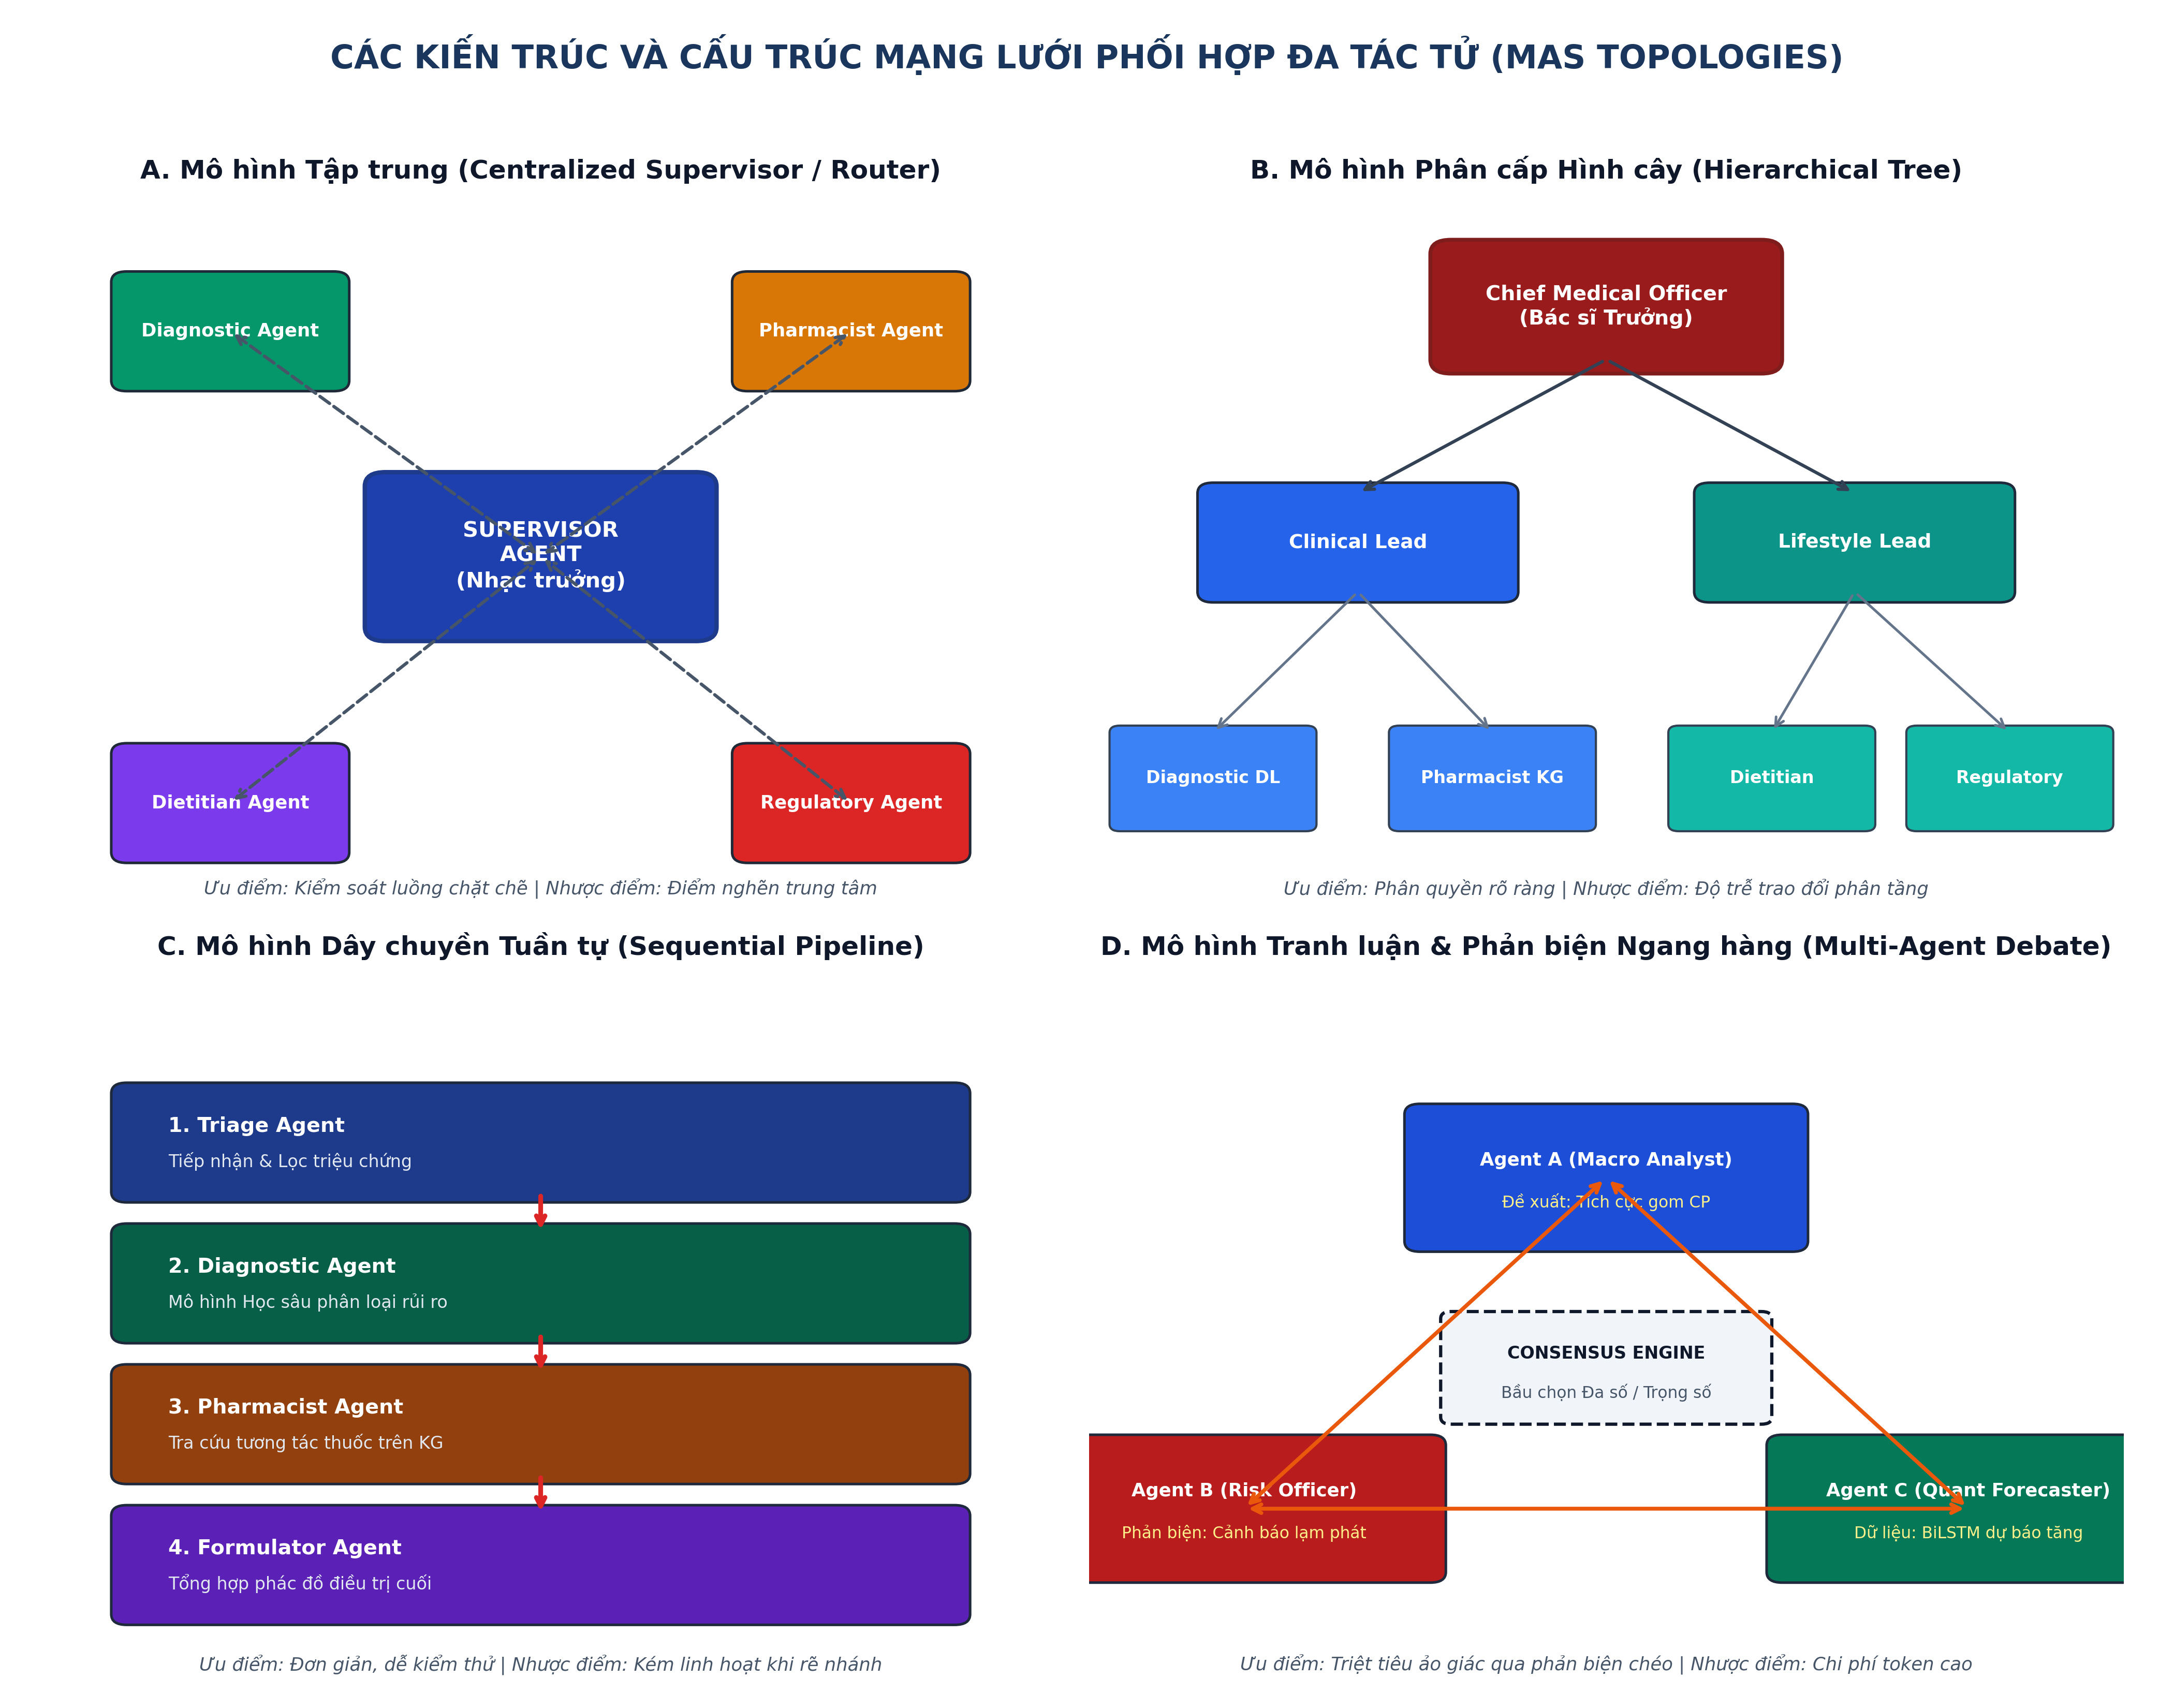
\includegraphics[width=0.96\textwidth]{images/fig601_mas_architecture_taxonomy.png}
    \caption{Phân loại các hình thái kiến trúc Hệ Multi-Agent (MAS Architecture Taxonomy) trong các hệ thống thông minh hiện đại.}
    \label{fig:mas_taxonomy}
\end{figure}

\subsubsection{Các mô hình điều phối Multi-Agent và đối chuẩn Framework}
Việc tổ chức tương tác giữa các Agent có thể thực hiện theo nhiều hình thái (Topologies) khác nhau như mô tả trong Hình~\ref{fig:mas_taxonomy} và Hình~\ref{fig:mas_comms}:
\begin{enumerate}[leftmargin=1.2cm]
    \item \textbf{Điều phối tuần tự (Sequential Pipeline):} Đầu ra của Agent này là đầu vào của Agent tiếp theo. Phù hợp cho chu trình xử lý dữ liệu chuẩn từ Tiếp đón $\to$ Dự báo $\to$ Chẩn đoán $\to$ Dinh dưỡng.
    \item \textbf{Điều phối phân tầng (Hierarchical / Router-Worker):} Một Agent Điều phối trung tâm (Orchestrator) phân tích ngữ cảnh và quyết định định tuyến linh hoạt nhiệm vụ cho nhóm Agent phù hợp.
    \item \textbf{Vòng lặp Phản biện (Reflection / Guardian Loop):} Một Agent giám sát có thẩm quyền phủ quyết (Veto Power) để kiểm tra chéo và yêu cầu hiệu chỉnh khi phát hiện sai phạm chuyên môn.
\end{enumerate}

\begin{figure}[H]
    \centering
    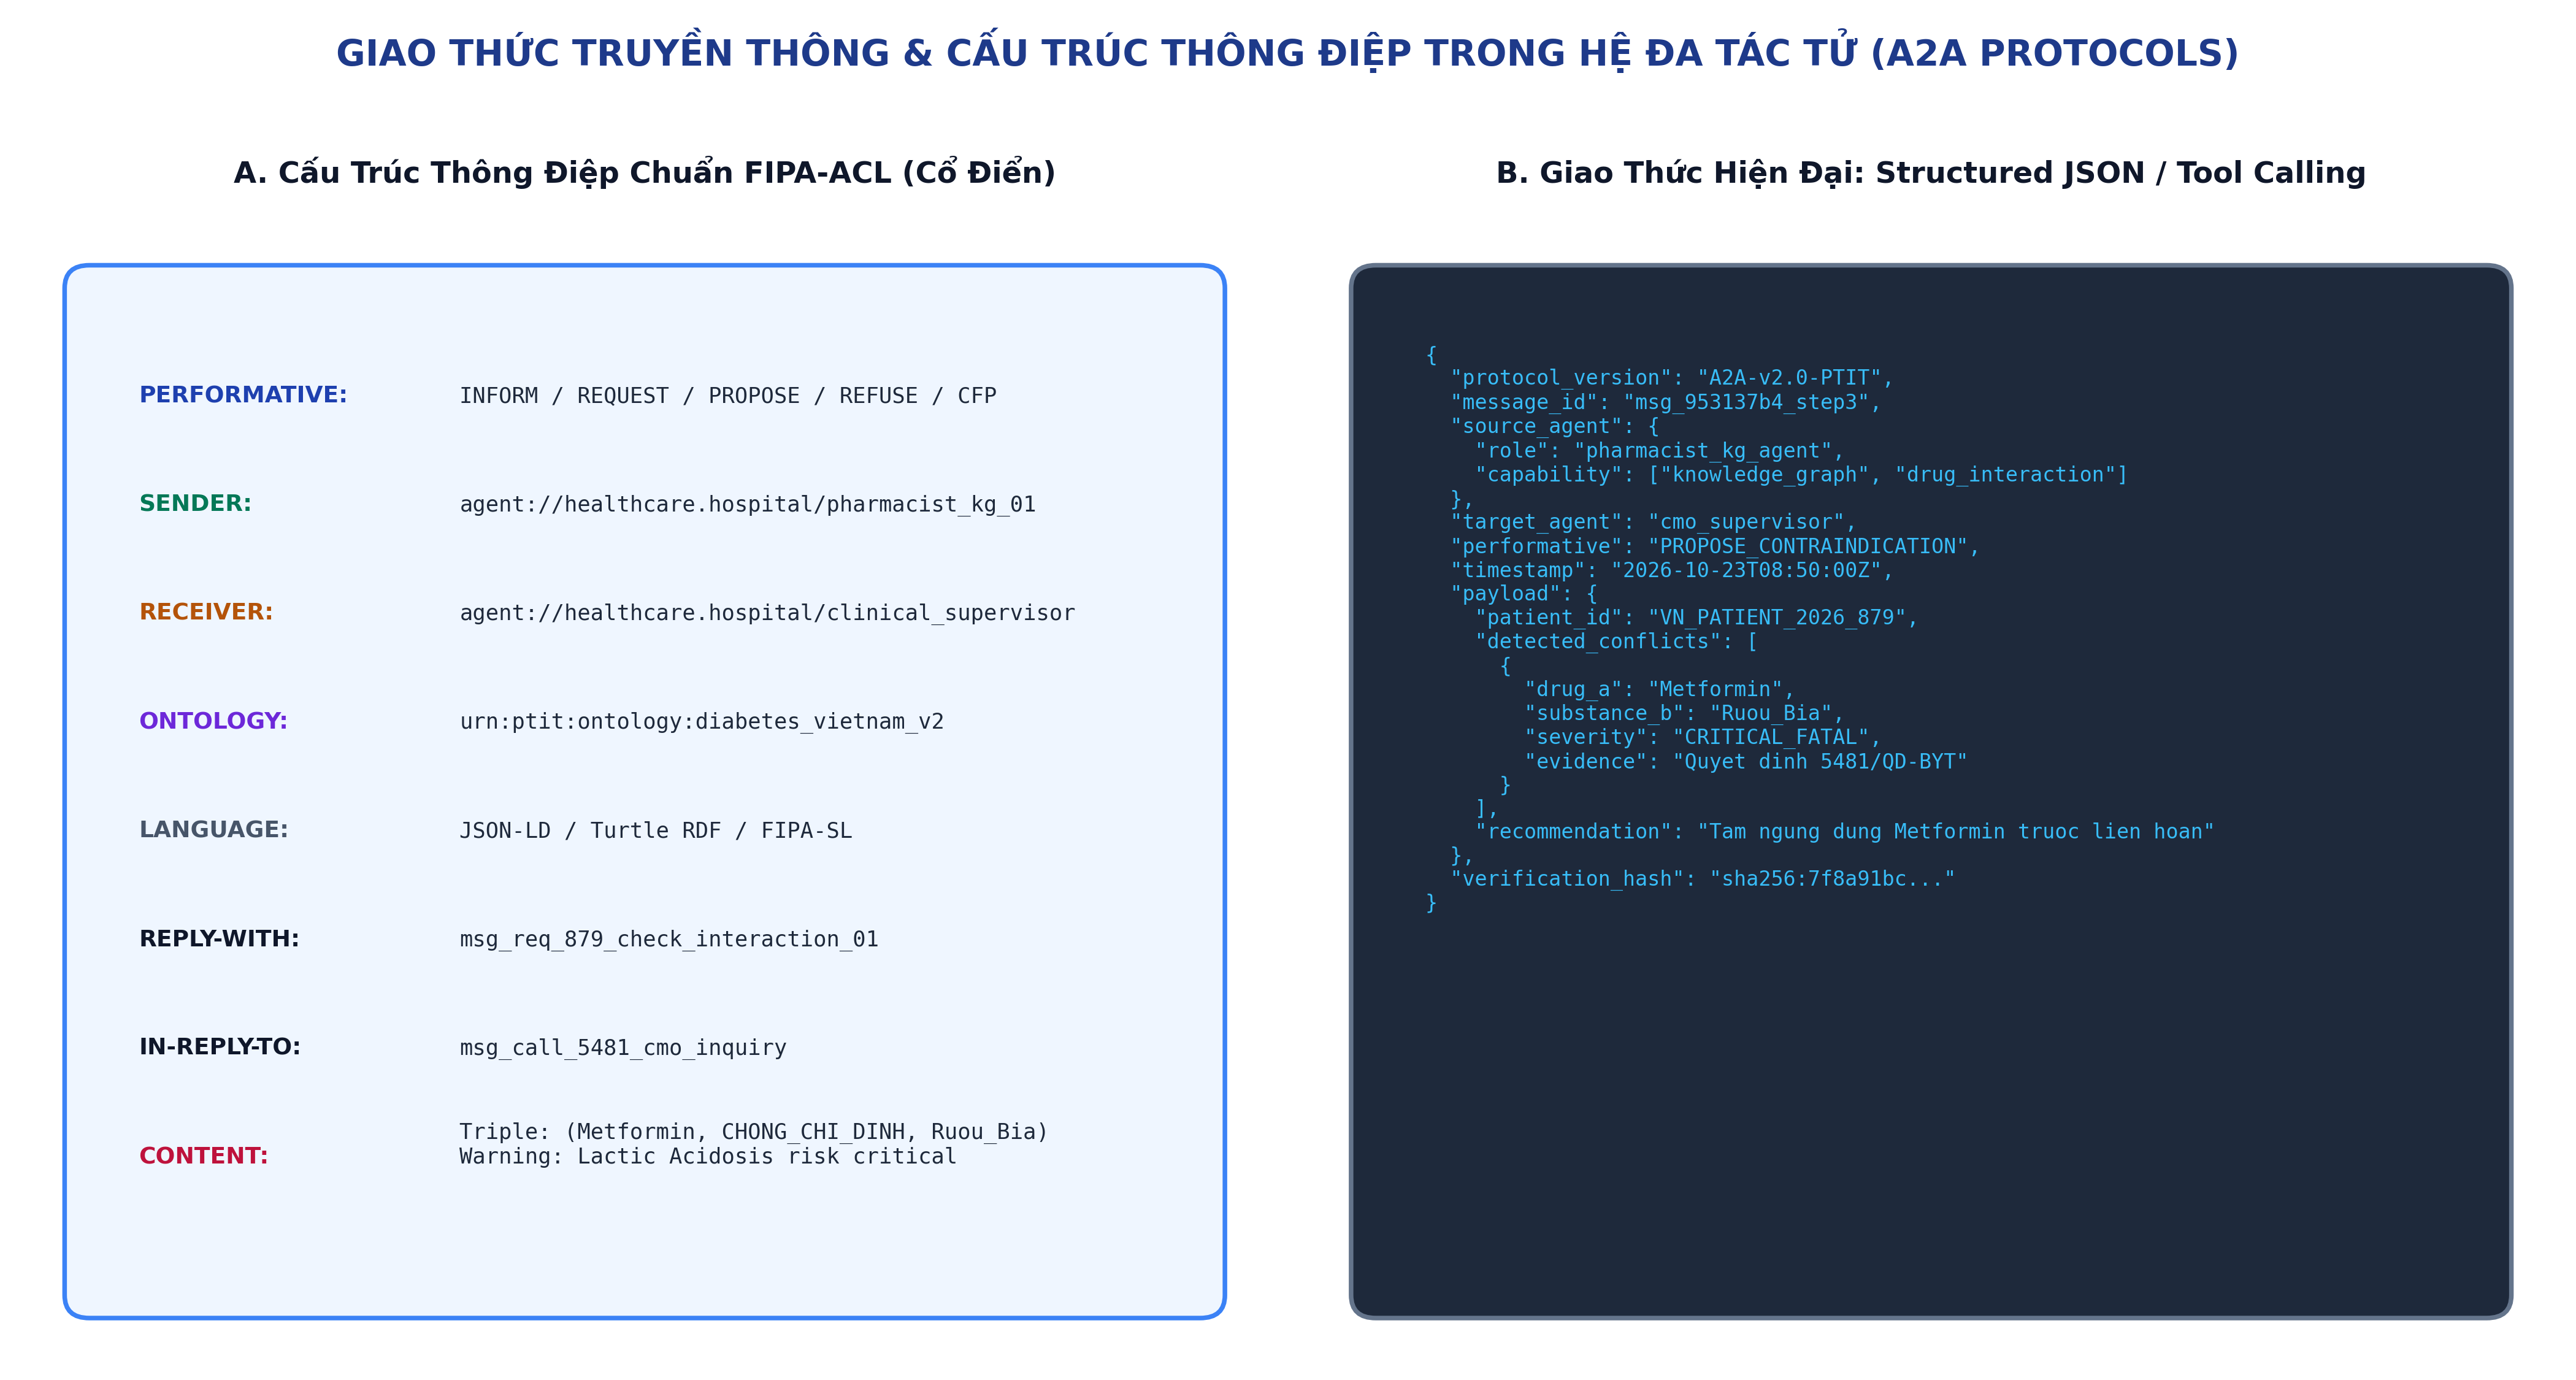
\includegraphics[width=0.96\textwidth]{images/fig602_mas_communication_protocols.png}
    \caption{Các giao thức truyền thông điệp (A2A Communication Protocols) và cơ chế chia sẻ bộ nhớ dùng chung trong Hệ Multi-Agent.}
    \label{fig:mas_comms}
\end{figure}

Bảng~\ref{tab:mas_frameworks} đối chuẩn kỹ thuật giữa các framework phát triển Multi-Agent hàng đầu hiện nay:

\begin{table}[H]
\centering
\footnotesize
\caption{Bảng đối chuẩn kỹ thuật giữa các nền tảng phát triển Hệ Multi-Agent}
\label{tab:mas_frameworks}
\begin{tabularx}{\textwidth}{@{} l Y Y Y Y @{}}
\toprule
\textbf{Tiêu chí} & \textbf{LangGraph} & \textbf{Microsoft AutoGen} & \textbf{CrewAI} & \textbf{DiaAgent-MAS (Hệ thống đề xuất)} \\
\midrule
Mô hình Trọng tâm & Đồ thị trạng thái có chu trình (Cyclic StateGraph) & Hội thoại nhóm đàm thoại (Conversable GroupChat) & Đóng vai tổ chức nhân sự (Role-Playing Crew) & Kiến trúc Hỗn hợp: Pipeline kết hợp Router \& Reflection Guardian \\
Cơ chế Lưu trữ & State dict tuần hoàn & Lịch sử tin nhắn Chat & Ngữ cảnh chia sẻ Task & Schema cấu trúc nghiêm ngặt (Pydantic Global State) \\
Kiểm soát Luồng & Cực cao (Điều kiện Edge) & Trung bình (Dựa vào LLM) & Trung bình (Tuần tự/Phân cấp) & Cực cao: Dual-mode Clinical Routing (Khóa/Mở ML xác định) \\
An toàn Y tế & Cần cấu hình ngoài & Dễ bị ảo giác chéo & Khó kiểm soát nhánh lặp & Tích hợp sẵn Safety Guardian với thẩm quyền phủ quyết tuyệt đối \\
Độ trễ phản hồi & 12 -- 20 giây & 15 -- 30 giây & 15 -- 25 giây & 5 -- 7 giây (Nhờ tối ưu hóa trích xuất NER có cấu trúc) \\
\bottomrule
\end{tabularx}
\end{table}

\subsection{Học máy Dự báo Nguy cơ và Khả năng Giải thích (Explainable AI -- XAI)}

\subsubsection{Thuật toán LightGBM và các đột phá tối ưu hóa}
Để dự báo định lượng xác suất nguy cơ mắc đái tháo đường từ các chỉ số sinh hóa máu và thể trạng, mô hình \textbf{LightGBM (Light Gradient Boosting Machine)} do Microsoft phát triển được lựa chọn làm mô hình học máy nòng cốt. Khác với các thuật toán Gradient Boosting truyền thống (như XGBoost hay CatBoost) duyệt qua toàn bộ mẫu dữ liệu và toàn bộ giá trị đặc trưng, LightGBM sở hữu hai cải tiến toán học vượt bậc:
\begin{enumerate}[leftmargin=1.2cm]
    \item \textbf{Gradient-based One-Side Sampling (GOSS):} Nhận thấy rằng các mẫu có độ dốc đạo hàm (Gradient) lớn đóng góp nhiều hơn vào việc giảm hàm mất mát, GOSS giữ lại toàn bộ các mẫu có độ dốc lớn nhất (tỷ lệ $a$), và chỉ lấy mẫu ngẫu nhiên một tỷ lệ nhỏ $b$ các mẫu có độ dốc thấp. Để bù đắp cho sự thay đổi phân phối dữ liệu, các mẫu có độ dốc thấp được nhân thêm một trọng số bù $\frac{1-a}{b}$ khi tính toán độ lợi thông tin (Information Gain):
    \begin{equation}
        \tilde{V}_j(d) = \frac{1}{n} \left( \frac{\left( \sum_{x_i \in A_l} g_i + \frac{1-a}{b} \sum_{x_i \in B_l} g_i \right)^2}{n_{l}^j(d)} + \frac{\left( \sum_{x_i \in A_r} g_i + \frac{1-a}{b} \sum_{x_i \in B_r} g_i \right)^2}{n_{r}^j(d)} \right)
    \end{equation}
    Nhờ đó, mô hình tập trung học từ các ca bệnh khó mà vẫn đảm bảo tính không thiên lệch (unbiased estimation) của phân phối mẫu.
    \item \textbf{Exclusive Feature Bundling (EFB):} Trong các tập dữ liệu lâm sàng lớn, nhiều đặc trưng rời rạc (One-hot encoding) có tính chất loại trừ lẫn nhau (hiếm khi đồng thời nhận giá trị khác 0). EFB gộp các đặc trưng này thành một đặc trưng dày đặc duy nhất (Dense Bundle) thông qua bài toán tô màu đồ thị, giúp giảm mạnh số chiều không gian mà không làm mất mát thông tin.
    \item \textbf{Chiến lược phát triển cây theo chiều sâu (Leaf-wise Tree Growth):} Thay vì phát triển cây cân bằng theo từng tầng (Level-wise) như XGBoost, LightGBM lựa chọn nút lá có độ giảm tổn thất lớn nhất để phân nhánh, giúp đạt độ chuẩn xác cao hơn với cùng số lượng lá quy định.
\end{enumerate}

Hàm mất mát Log-loss nhị phân của bài toán dự đoán nguy cơ đái tháo đường ($y_i \in \{0, 1\}$) được biểu diễn bởi:
\begin{equation}
    \mathcal{L}(y, \hat{y}) = - \frac{1}{N} \sum_{i=1}^N \left[ y_i \log(\hat{y}_i) + (1 - y_i) \log(1 - \hat{y}_i) \right] + \sum_{k=1}^K \Omega(f_k)
\end{equation}
trong đó $\hat{y}_i = \sigma(\sum_{k=1}^K f_k(x_i))$ là xác suất dự báo sau hàm Sigmoid, và $\Omega(f_k) = \gamma T + \frac{1}{2} \lambda \|w\|^2$ là thành phần điều chuẩn chống quá khớp (Overfitting).

\subsubsection{Lý thuyết Giá trị Shapley và Phương pháp Giải thích SHAP}
Trong y tế, một mô hình đạt độ chính xác cao nhưng hoạt động như một "hộp đen" hoàn toàn không thể được đưa vào ứng dụng thực tiễn vì bác sĩ và bệnh nhân không thể biết được yếu tố nào đang thúc đẩy kết luận. Để giải quyết vấn đề này, hệ thống ứng dụng phương pháp \textbf{SHAP (SHapley Additive exPlanations)} dựa trên nền tảng lý thuyết trò chơi hợp tác của Lloyd Shapley (giải Nobel Kinh tế 2012).

Giá trị Shapley $\phi_j(x)$ biểu diễn mức đóng góp công bằng của đặc trưng thứ $j$ vào sai khác giữa giá trị dự báo của mẫu $f(x)$ so với kỳ vọng trung bình toàn bộ tập dữ liệu $\mathbb{E}[f(X)]$:
\begin{equation}
    \phi_j(x) = \sum_{S \subseteq F \setminus \{j\}} \frac{|S|! (|F| - |S| - 1)!}{|F|!} \left[ f(S \cup \{j\}) - f(S) \right]
\end{equation}
trong đó:
\begin{itemize}[leftmargin=1.2cm]
    \item $F$ là toàn bộ tập hợp $M$ đặc trưng đầu vào ($|F| = M$).
    \item $S$ là tập hợp con các đặc trưng không chứa đặc trưng $j$.
    \item $f(S)$ là giá trị dự đoán khi chỉ biết các đặc trưng trong $S$.
    \item Phân số $\frac{|S|! (|F| - |S| - 1)!}{|F|!}$ là xác suất hoán vị xuất hiện của liên minh $S$.
\end{itemize}

Mô hình giải thích SHAP thỏa mãn 4 tính chất toán học quan trọng:
\begin{enumerate}[leftmargin=1.2cm]
    \item \textbf{Tính cộng tính địa phương (Local Accuracy):} Tổng giá trị SHAP của tất cả đặc trưng cộng với giá trị cơ sở bằng đúng đầu ra của mô hình: $f(x) = \phi_0 + \sum_{j=1}^M \phi_j(x)$.
    \item \textbf{Tính khuyết thiếu (Missingness):} Đặc trưng không có mặt trong đầu vào nhận giá trị $\phi_j = 0$.
    \item \textbf{Tính đối xứng (Symmetry):} Nếu hai đặc trưng $j$ và $k$ có đóng góp tương đương vào mọi liên minh thì $\phi_j = \phi_k$.
    \item \textbf{Tính đơn điệu (Monotonicity):} Nếu mô hình thay đổi sao cho đóng góp biên của đặc trưng $j$ luôn tăng hoặc giữ nguyên thì giá trị Shapley $\phi_j$ chắc chắn không giảm.
\end{enumerate}

Nhờ SHAP, Agent Dự báo (Risk Prediction Agent) có thể trích xuất chính xác Top-3 yếu tố rủi ro hàng đầu (ví dụ: chỉ số $\text{HbA1c} = 7.8\%$ đóng góp $+0.42$ vào xác suất bệnh; chỉ số Glucose đói $155\text{ mg/dL}$ đóng góp $+0.31$) để giải thích minh bạch cho người bệnh.

\subsection{Đồ thị Tri thức Y tế (Clinical Knowledge Graph) và Phác đồ Lâm sàng}

\subsubsection{Cấu trúc Biểu diễn Tri thức Bộ ba RDF}
Để đảm bảo các Agent không bị ảo giác về mặt y khoa, tri thức y tế cần được cấu trúc hóa dưới dạng \textbf{Đồ thị Tri thức (Knowledge Graph -- KG)}. Đồ thị tri thức biểu diễn các mối quan hệ ngữ nghĩa thông qua các bộ ba (Triples) theo chuẩn RDF:
\begin{equation}
    \mathcal{KG} = \{ (h, r, t) \mid h, t \in \mathcal{E}, \ r \in \mathcal{R}_{rel} \}
\end{equation}
trong đó $h$ là thực thể đầu (Head), $t$ là thực thể cuối (Tail), và $r$ là mối quan hệ định hướng (Relation).

\begin{figure}[H]
    \centering
    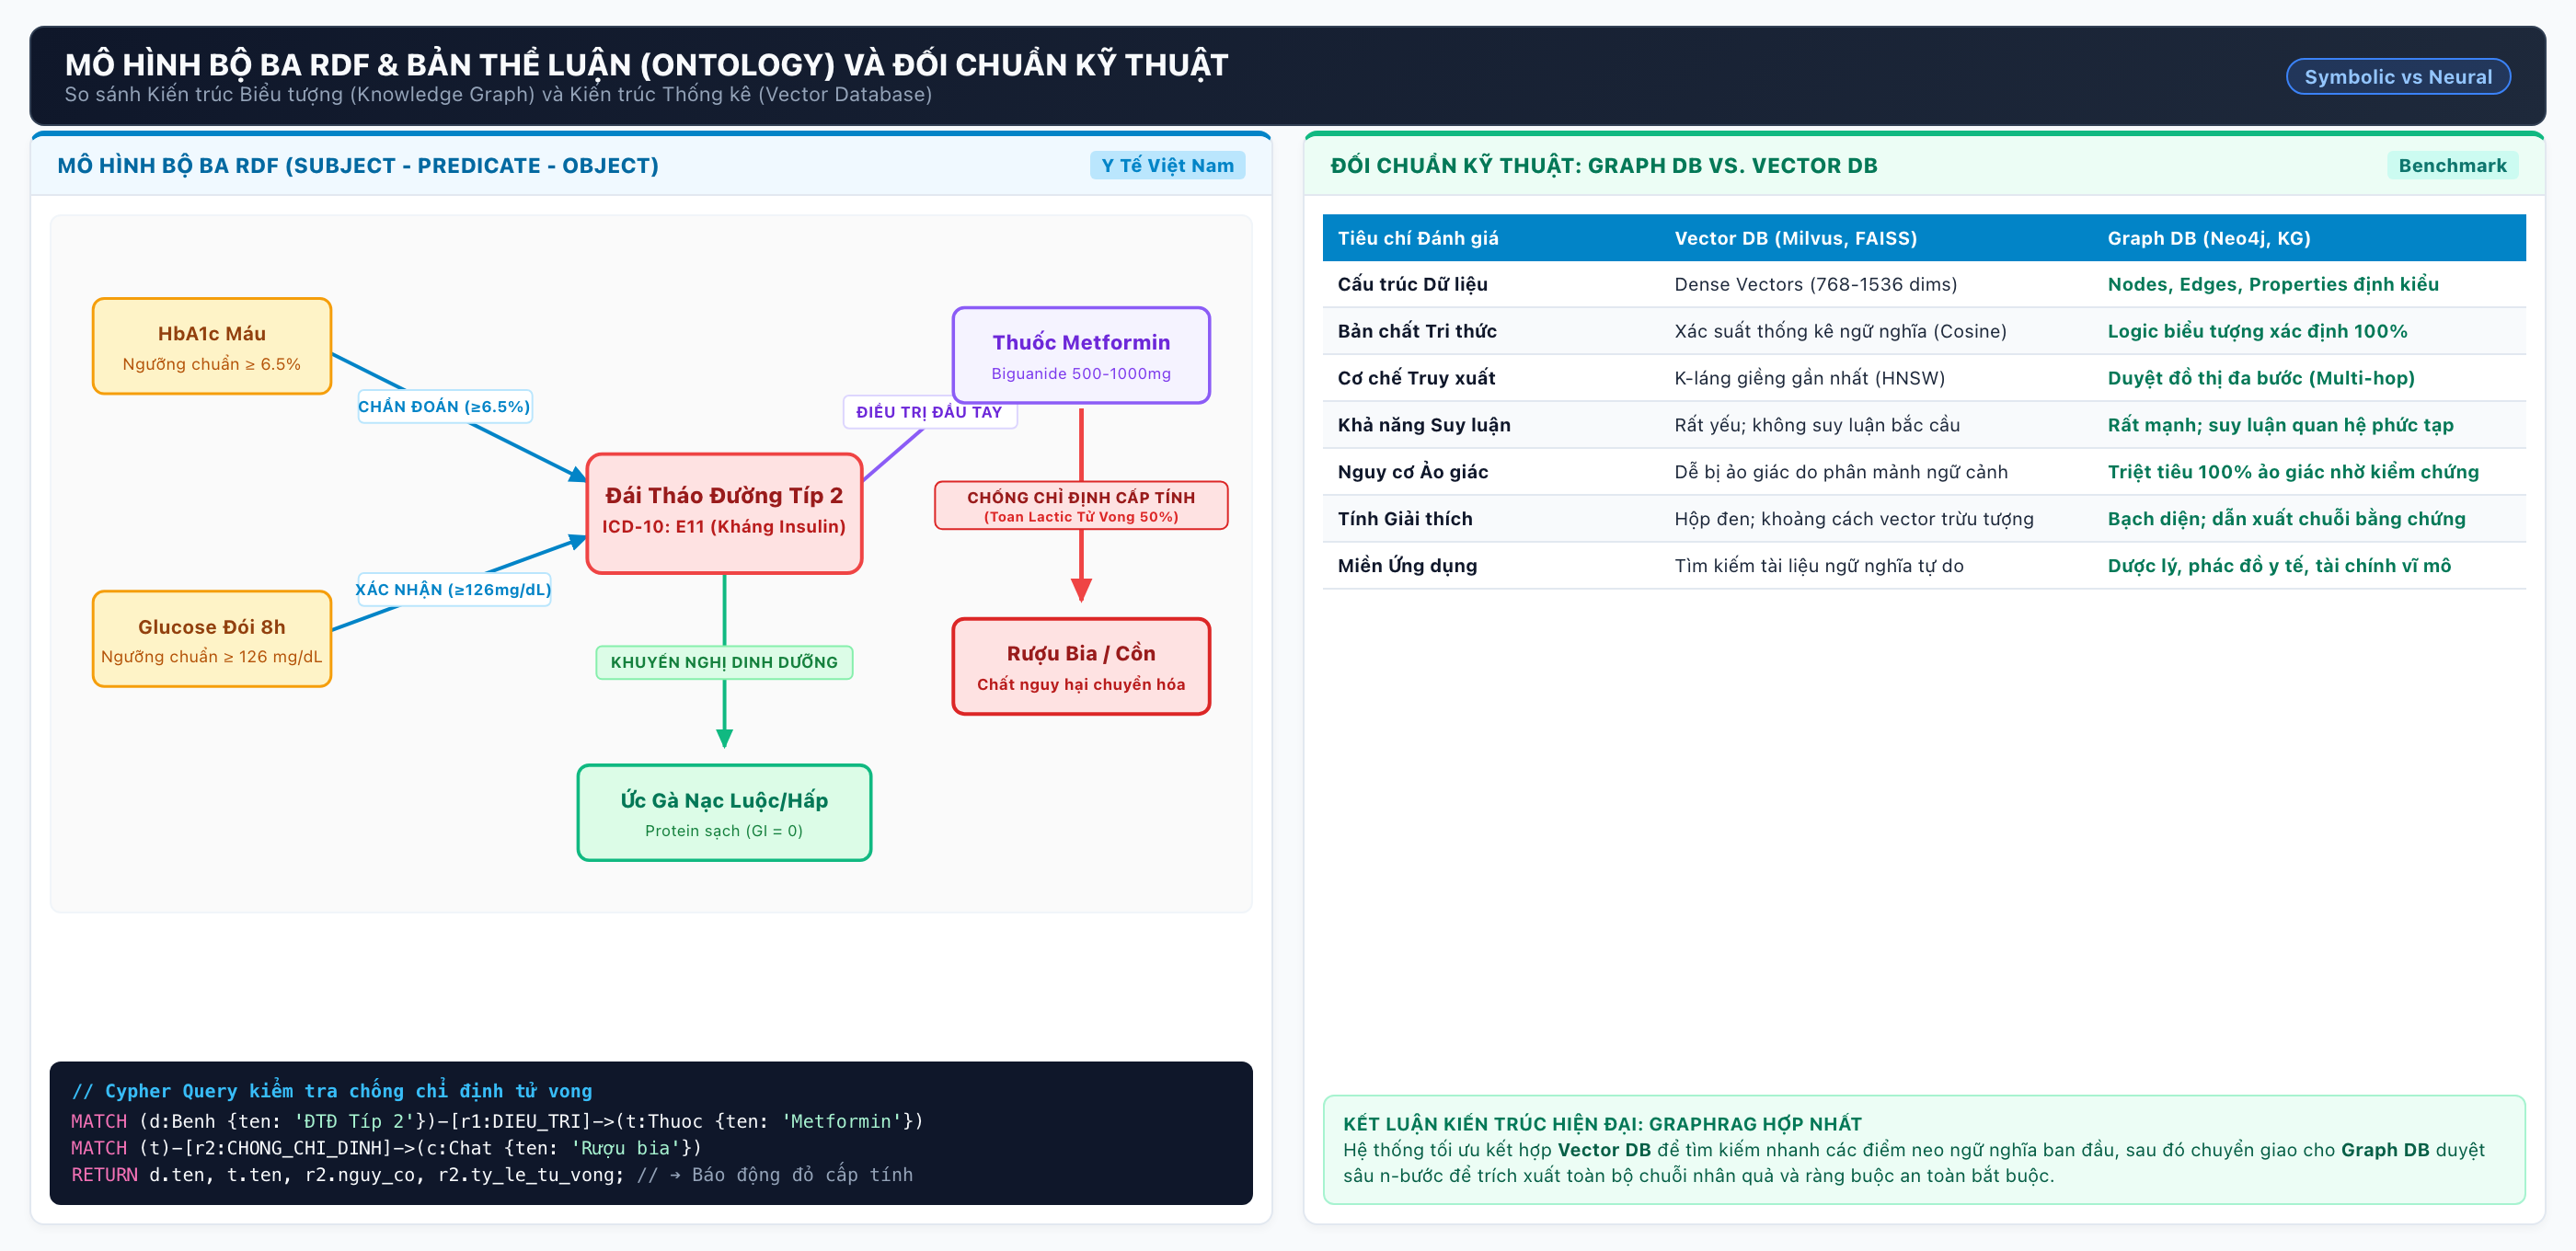
\includegraphics[width=0.96\textwidth]{images/fig702_knowledge_graph_triples_ontology.png}
    \caption{Mô hình hóa Bản thể học (Ontology) và Cấu trúc Bộ ba Tri thức (RDF Triples) trong Y tế Lâm sàng.}
    \label{fig:kg_triples}
\end{figure}

Trong bài toán đái tháo đường, Ontology đồ thị bao gồm các lớp thực thể: $\mathcal{E} = \{\text{Bệnh lý}, \text{Triệu chứng}, \text{Thuốc}, \text{Chỉ số Xét nghiệm}, \text{Thực phẩm}, \text{Chống chỉ định}\}$; và các mối quan hệ lâm sàng: $\mathcal{R}_{rel} = \{\text{has\_symptom}, \text{indicated\_for}, \text{contraindicated\_with}, \text{adverse\_interaction}, \text{requires\_lab}\}$.

\begin{figure}[H]
    \centering
    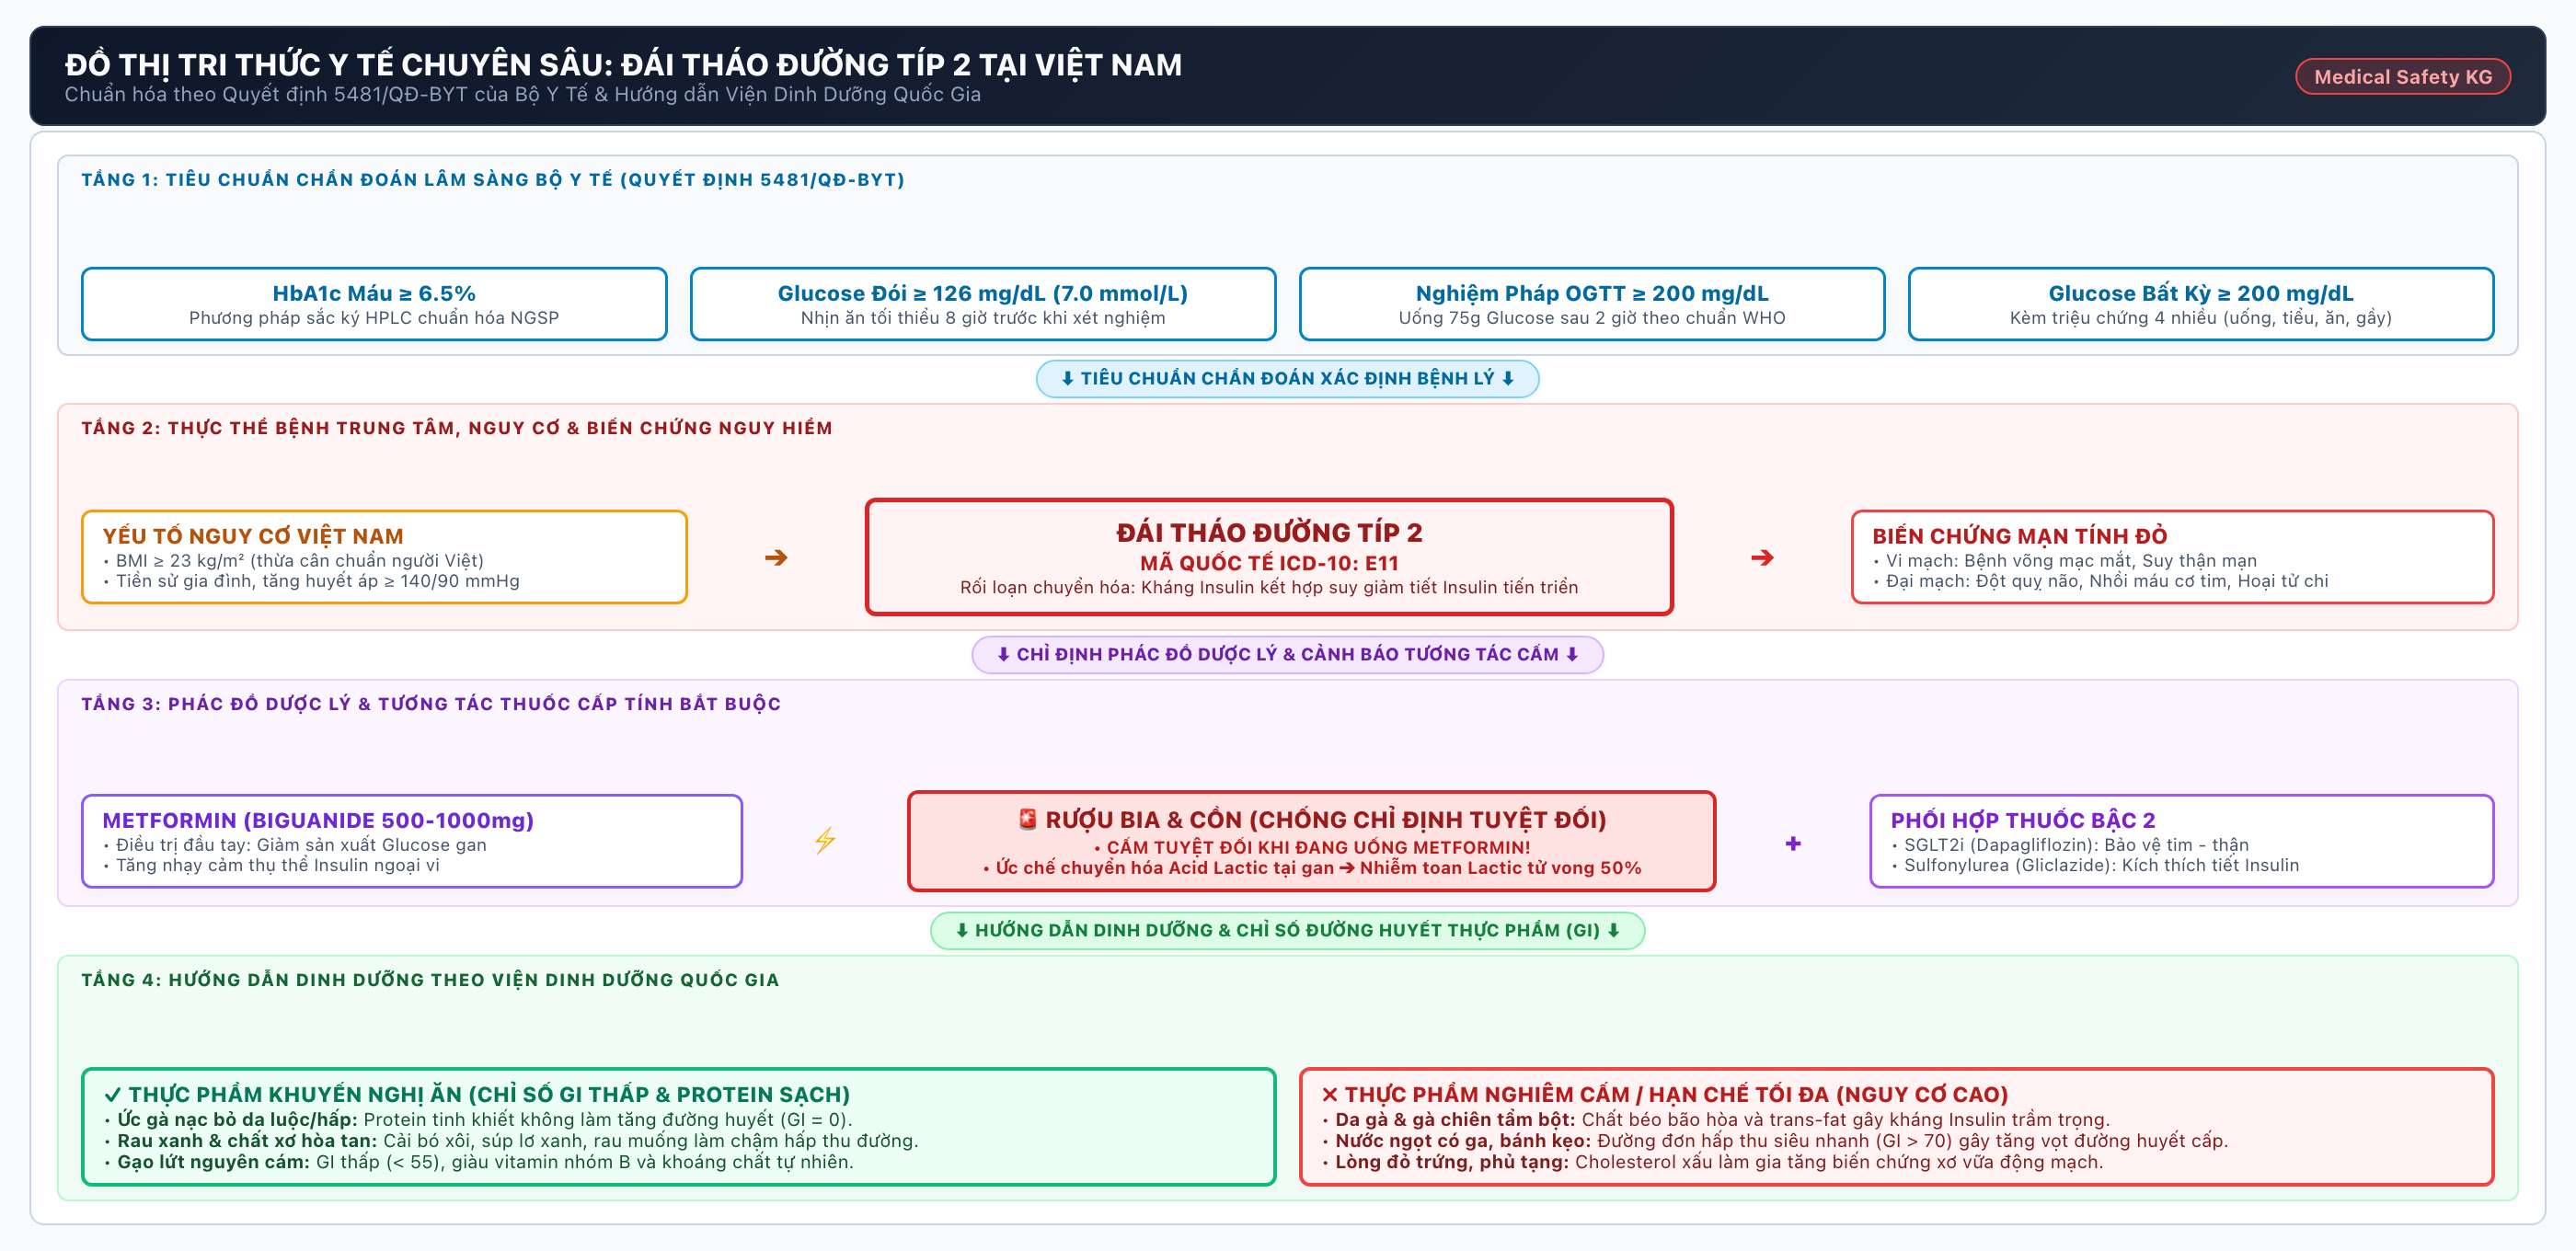
\includegraphics[width=0.96\textwidth]{images/fig704_diabetes_vietnam_knowledge_graph.png}
    \caption{Đồ thị Tri thức Chuyên biệt Quản trị Bệnh Đái Tháo Đường tại Việt Nam: Phác đồ Bộ Y Tế 5481, Tương tác Dược lý và Dinh dưỡng Thực phẩm Việt.}
    \label{fig:diabetes_kg}
\end{figure}

\subsubsection{Không Gian Biểu Diễn Vector Tiềm Ẩn (Node \& Link Embeddings)}
Để hỗ trợ các tác vụ suy luận ngữ nghĩa nhanh và tìm kiếm lân cận tương đồng trong chẩn đoán, toàn bộ 143 nút thực thể và 271 mối liên kết trong Đồ thị Tri thức Neo4j DiaAgent-MAS được chiếu vào một \textbf{Không gian Vector Nhúng Tiềm ẩn (Latent Node Embedding Space)} thông qua thuật toán bố trí lực lò xo Force-Directed Graph Layout kết hợp vector tiên nghiệm phân cụm ngữ nghĩa (Semantic Clustering Priors) (Hình~\ref{fig:kg_node_embeddings}).

Trong không gian nhúng 2 chiều:
\begin{itemize}[leftmargin=1.2cm]
    \item Các nút có cùng vai trò chuyên môn tự động hội tụ thành các cụm mật độ cao (Dense Clusters) được bao quanh bởi các đường bao mây: Cụm Dược chất phác đồ Bộ Y Tế và ADA (Metformin, Gliclazide, SGLT-2i, DPP-4i, GLP-1 RA, Insulin), Cụm 30 Biệt dược và Thiết bị y tế thương mại FPT Long Châu (Glucophage, Diamicron, Jardiance, Forxiga, Máy đo và que thử Accu-Chek, Sữa Glucerna), Cụm 14 Chỉ số sinh học xét nghiệm (HbA1c, FPG, OGTT, RPG, eGFR, Creatinine, UACR, BMI, Huyết áp, Lipid), Cụm Triệu chứng lâm sàng kinh điển (Hội chứng 4 nhiều, nhìn mờ, tê bì bàn chân, vết thương lâu lành từ Vinmec), Cụm Bệnh lý và Biến chứng đa cơ quan (CKD, ASCVD, Suy tim, Võng mạc, Thần kinh, Loét bàn chân), Cụm Dinh dưỡng 29 món ăn Việt Nam (NIN) và Cụm Cảnh báo an toàn (Nhiễm toan Lactic, Hạ đường huyết, Toan Ceton).
    \item Các liên kết quan hệ định hướng (\texttt{TREATS}, \texttt{CONTRAINDICATED\_IN}, \texttt{RISK\_OF}, \texttt{HIGHLY\_RECOMMENDED\_FOR}, \texttt{DIAGNOSED\_BY}, \texttt{HAS\_SYMPTOM}, \texttt{CAN\_BE\_REPLACED\_BY}, \texttt{DISPENSED\_AS\_PRODUCT}) kết nối trực tiếp các vector nhúng, phản ánh toàn vẹn tô-pô phác đồ và cơ chế rà soát an toàn dược lý đa tầng của hệ thống.
\end{itemize}

\begin{figure}[H]
    \centering
    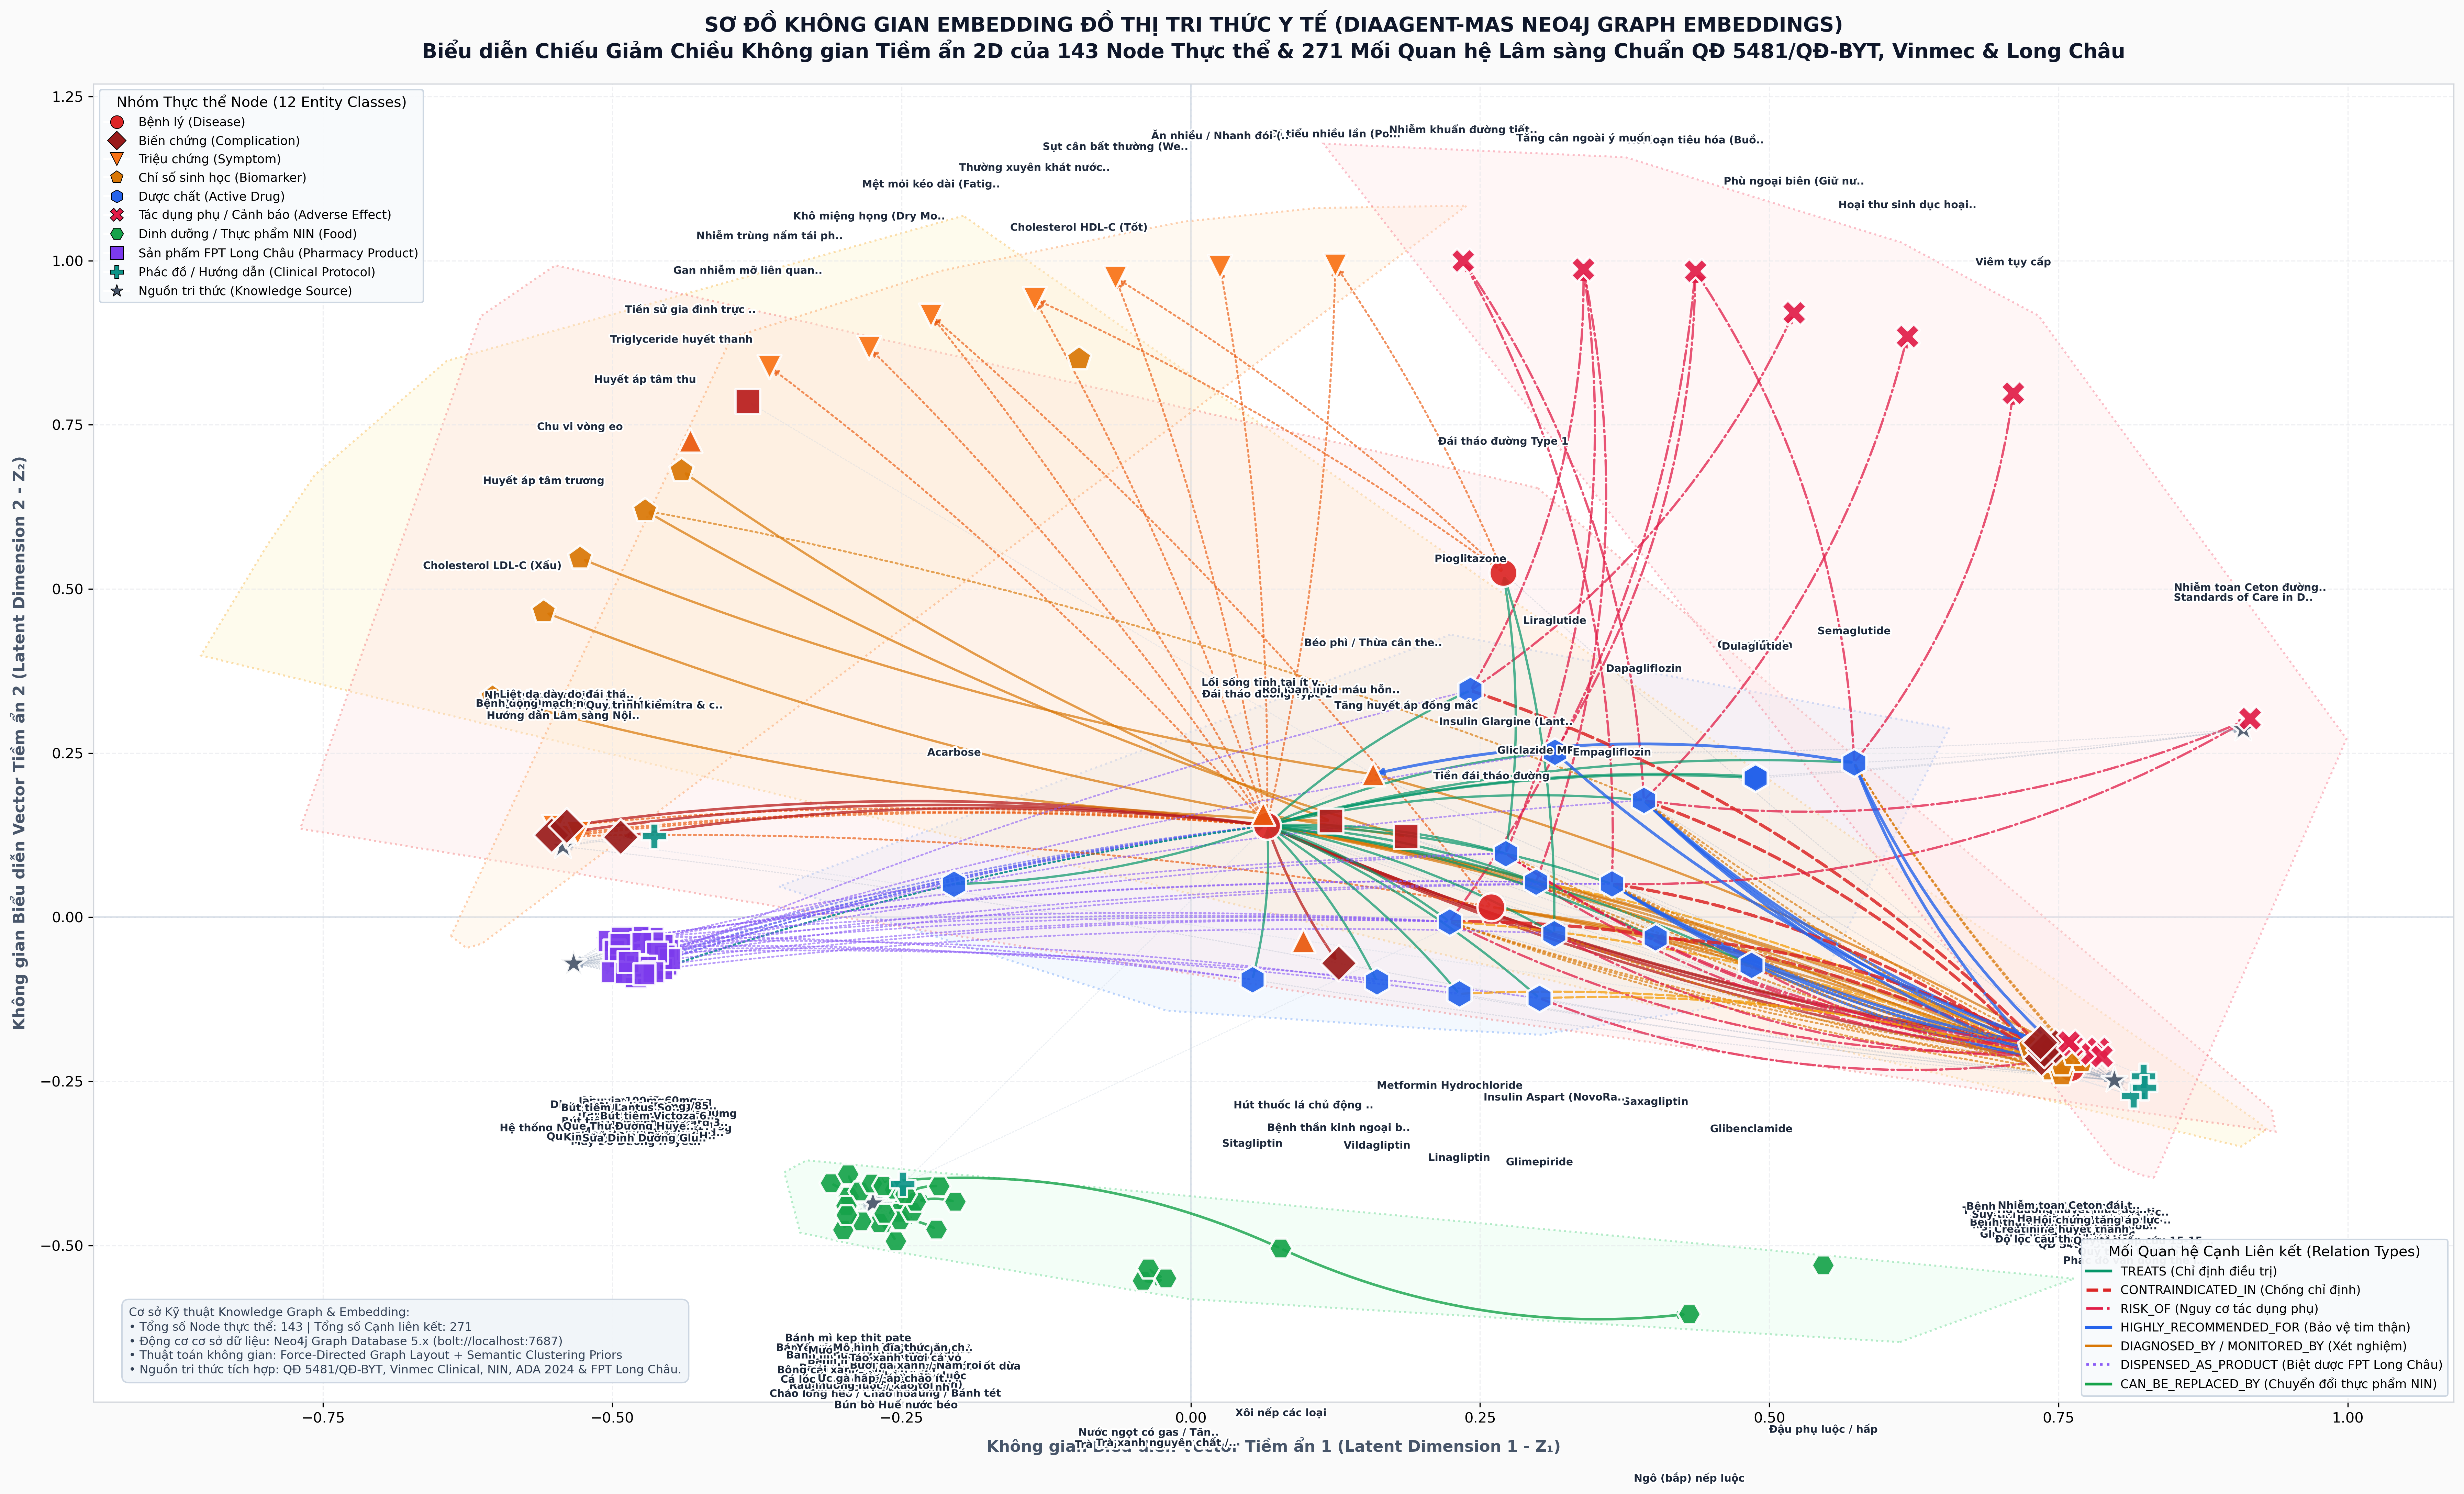
\includegraphics[width=0.98\textwidth]{images/fig_kg_node_embeddings.png}
    \caption{Không Gian Vector Embedding 2D (Force-Directed Graph Layout \& Semantic Clustering) Biểu Diễn 143 Node Thực Thể và 271 Mối Quan Hệ Liên Kết Lâm Sàng trong Đồ Thị Tri Thức Neo4j DiaAgent-MAS.}
    \label{fig:kg_node_embeddings}
\end{figure}

\subsubsection{Chuẩn hóa Phác đồ Đái Tháo Đường Type 2 theo Quyết định 5481/QĐ-BYT}
Hệ thống DiaAgent-MAS số hóa và áp dụng nghiêm ngặt các quy định chuyên môn từ \textbf{Quyết định số 5481/QĐ-BYT ngày 30/12/2020 của Bộ Trưởng Bộ Y Tế Việt Nam} về việc ban hành tài liệu chuyên môn "Hướng dẫn chẩn đoán và điều trị đái tháo đường típ 2":
\begin{enumerate}[leftmargin=1.2cm]
    \item \textbf{Tiêu chuẩn vàng khẳng định chẩn đoán đái tháo đường:}
    Bắt buộc phải dựa vào kết quả xét nghiệm định lượng từ mẫu huyết tương tĩnh mạch thực hiện tại phòng xét nghiệm chuẩn, thỏa mãn ít nhất một trong 4 tiêu chuẩn:
    \begin{itemize}[leftmargin=0.8cm]
        \item Glucose huyết tương lúc đói (Fasting Plasma Glucose -- FPG) $\ge 126\text{ mg/dL}$ ($\ge 7.0\text{ mmol/L}$) sau ít nhất 8 giờ nhịn ăn.
        \item Glucose huyết tương ở thời điểm 2 giờ sau nghiệm pháp dung nạp 75g glucose đường uống (OGTT) $\ge 200\text{ mg/dL}$ ($\ge 11.1\text{ mmol/L}$).
        \item $\text{HbA1c} \ge 6.5\%$ ($48\text{ mmol/mol}$) thực hiện theo phương pháp chuẩn hóa NGSP/DCCT.
        \item Bệnh nhân có các triệu chứng lâm sàng kinh điển của tăng đường huyết (khát nhiều, uống nhiều, tiểu nhiều, sụt cân không rõ nguyên nhân) kèm theo một mẫu glucose huyết tương bất kỳ $\ge 200\text{ mg/dL}$ ($\ge 11.1\text{ mmol/L}$).
    \end{itemize}
    \begin{tcolorbox}[colback=warnbg,colframe=warnframe,title=Nguyên tắc An toàn Bắt buộc theo QĐ 5481/QĐ-BYT]
    Tuyệt đối KHÔNG sử dụng các triệu chứng lâm sàng đơn thuần hoặc que thử mao mạch nhanh để khẳng định chẩn đoán xác định đái tháo đường. Khi bệnh nhân chưa có kết quả xét nghiệm máu định lượng, hệ thống CHỈ ĐƯỢC PHÉP xếp bệnh nhân vào diện "Sàng lọc nguy cơ" và hướng dẫn đi làm xét nghiệm, tuyệt đối KHÔNG chỉ định thuốc điều trị đặc trị.
    \end{tcolorbox}
    \item \textbf{Phác đồ điều trị và các chống chỉ định thuốc cốt tử:}
    \begin{itemize}[leftmargin=0.8cm]
        \item \textbf{Thuốc đầu tay (First-line Therapy):} \textit{Metformin} là lựa chọn ưu tiên hàng đầu ngay khi được chẩn đoán đái tháo đường típ 2, kết hợp với thay đổi lối sống.
        \item \textbf{Chống chỉ định suy giảm chức năng thận của Metformin:}
        Theo QĐ 5481/QĐ-BYT, việc sử dụng Metformin bắt buộc phải căn cứ vào Độ lọc cầu thận ước tính (eGFR):
        \begin{equation}
            \text{eGFR} = \begin{cases}
                \ge 60\text{ mL/phút/1.73m}^2: & \text{Liều tối đa 2000 -- 2500 mg/ngày (An toàn)} \\
                45 \le \text{eGFR} < 60: & \text{Liều tối đa 1500 mg/ngày, theo dõi mỗi 3--6 tháng} \\
                30 \le \text{eGFR} < 45: & \text{Liều tối đa 1000 mg/ngày (Thận trọng, giảm 50\% liều)} \\
                < 30\text{ mL/phút/1.73m}^2: & \textbf{CHỐNG CHỈ ĐỊNH TUYỆT ĐỐI}
            \end{cases}
        \end{equation}
        \item \textbf{Tương tác nghiêm trọng giữa Metformin và Rượu bia:}
        Cồn (Ethanol) ức chế quá trình tân tạo đường tại gan và cạnh tranh chuyển hóa với acid lactic, làm tăng đột biến nguy cơ \textbf{Nhiễm toan Acid Lactic (Lactic Acidosis)} cấp tính -- một biến chứng có tỷ lệ tử vong lên tới 50\%. Bệnh nhân đang sử dụng Metformin bắt buộc phải kiêng tuyệt đối rượu bia.
    \end{itemize}
\end{enumerate}

\subsubsection{Cơ sở Dữ liệu Dinh dưỡng theo Viện Dinh Dưỡng Quốc Gia (NIN)}
Hệ thống DiaAgent-MAS tích hợp bảng thành phần dinh dưỡng thực phẩm Việt Nam của Viện Dinh Dưỡng Quốc Gia (NIN). Chế độ can thiệp dinh dưỡng y khoa (Medical Nutrition Therapy -- MNT) cho người bệnh đái tháo đường tại Việt Nam được cá nhân hóa dựa trên:
\begin{itemize}[leftmargin=1.2cm]
    \item \textbf{Tổng năng lượng hàng ngày (Total Daily Energy Expenditure -- TDEE):}
    Tính toán dựa trên chỉ số khối cơ thể (BMI) và mức độ tiêu hao năng lượng do hoạt động thể lực:
    \begin{equation}
        E_{target} = W_{ideal} \times k_{activity}
    \end{equation}
    trong đó cân nặng lý tưởng của người Việt Nam tính theo công thức: $W_{ideal} = (\text{Chiều cao (cm)} - 100) \times 0.9$. Hệ số vận động $k_{activity} = 25\text{ kcal/kg}$ với người nằm viện hoặc ít vận động; $k_{activity} = 30\text{ kcal/kg}$ với lao động nhẹ; và $35\text{ kcal/kg}$ với lao động vừa. Đối với người thừa cân/béo phì ($\text{BMI} \ge 23\text{ kg/m}^2$ theo chuẩn châu Á IDI \& WPRO), năng lượng nạp vào giảm 500 kcal/ngày để hướng tới giảm 5--10\% trọng lượng cơ thể.
    \item \textbf{Tỷ lệ phân bổ các chất đa lượng (Macronutrient Distribution):}
    \begin{itemize}[leftmargin=0.8cm]
        \item Carbohydrate (Tinh bột): 50 -- 60\% tổng năng lượng. Ưu tiên tinh bột có chỉ số đường huyết thấp ($\text{GI} < 55$), giàu chất xơ hòa tan (gạo lứt, yến mạch, các loại đậu). Hạn chế tối đa carbohydrate hấp thu nhanh ($\text{GI} > 70$ như đường tinh luyện, nước ngọt, bánh mì trắng).
        \item Protein (Chất đạm): 15 -- 20\% tổng năng lượng ($1.0 - 1.2\text{ g/kg/ngày}$). Nếu có suy thận mạn ($\text{eGFR} < 60$), tỷ lệ đạm giảm xuống $0.8\text{ g/kg/ngày}$ để làm chậm tiến triển suy thận.
        \item Lipid (Chất béo): 20 -- 25\% tổng năng lượng. Chất béo bão hòa $< 7\%$, cholesterol $< 200\text{ mg/ngày}$, không sử dụng chất béo chuyển hóa (trans fat).
    \end{itemize}
\end{itemize}


% =========================================================================
% CHƯƠNG 2: THIẾT KẾ KIẾN TRÚC HỆ THỐNG DIAAGENT-MAS
% =========================================================================
\section{THIẾT KẾ KIẾN TRÚC HỆ THỐNG DIAAGENT-MAS}

\subsection{Kiến trúc Tổng thể và Cơ chế Điều phối Trung tâm}

\subsubsection{Sơ đồ Luồng Dữ liệu và Tương tác Đa Agent}
Kiến trúc nhận thức của hệ thống \textbf{DiaAgent-MAS} được xây dựng dựa trên nguyên lý điều phối hỗn hợp: kết hợp luồng tuần tự (Sequential Pipeline) có phân nhánh điều kiện (Conditional Branching) và vòng lặp phản biện an toàn (Reflection Guardian Loop). Toàn bộ hệ thống được chia thành 3 lớp chức năng cốt lõi:
\begin{enumerate}[leftmargin=1.2cm]
    \item \textbf{Lớp Giao tiếp \& Tiếp đón (Interaction \& Ingestion Layer):} Phụ trách hội thoại trực tiếp với người dùng, phân tích ý định (Intent Classification) và bóc tách thực thể lâm sàng có cấu trúc.
    \item \textbf{Lớp Trí tuệ Đa Agent Chuyên khoa (Specialized Multi-Agent Brain):} Gồm các Agent chuyên trách giải quyết từng khía cạnh y tế độc lập: dự báo nguy cơ học máy, chẩn đoán nội tiết, tính toán dinh dưỡng, huấn luyện lối sống và tra cứu dược phẩm thực tế.
    \item \textbf{Lớp Hộ vệ An toàn \& Kiểm chứng Phản biện (Safety Guardian \& Verification Layer):} Giám sát toàn bộ trạng thái, kiểm tra chéo các chống chỉ định y khoa theo phác đồ Bộ Y Tế, phát hiện ảo giác và phê duyệt kết quả cuối cùng trước khi phản hồi người dùng.
\end{enumerate}

\begin{figure}[H]
    \centering
    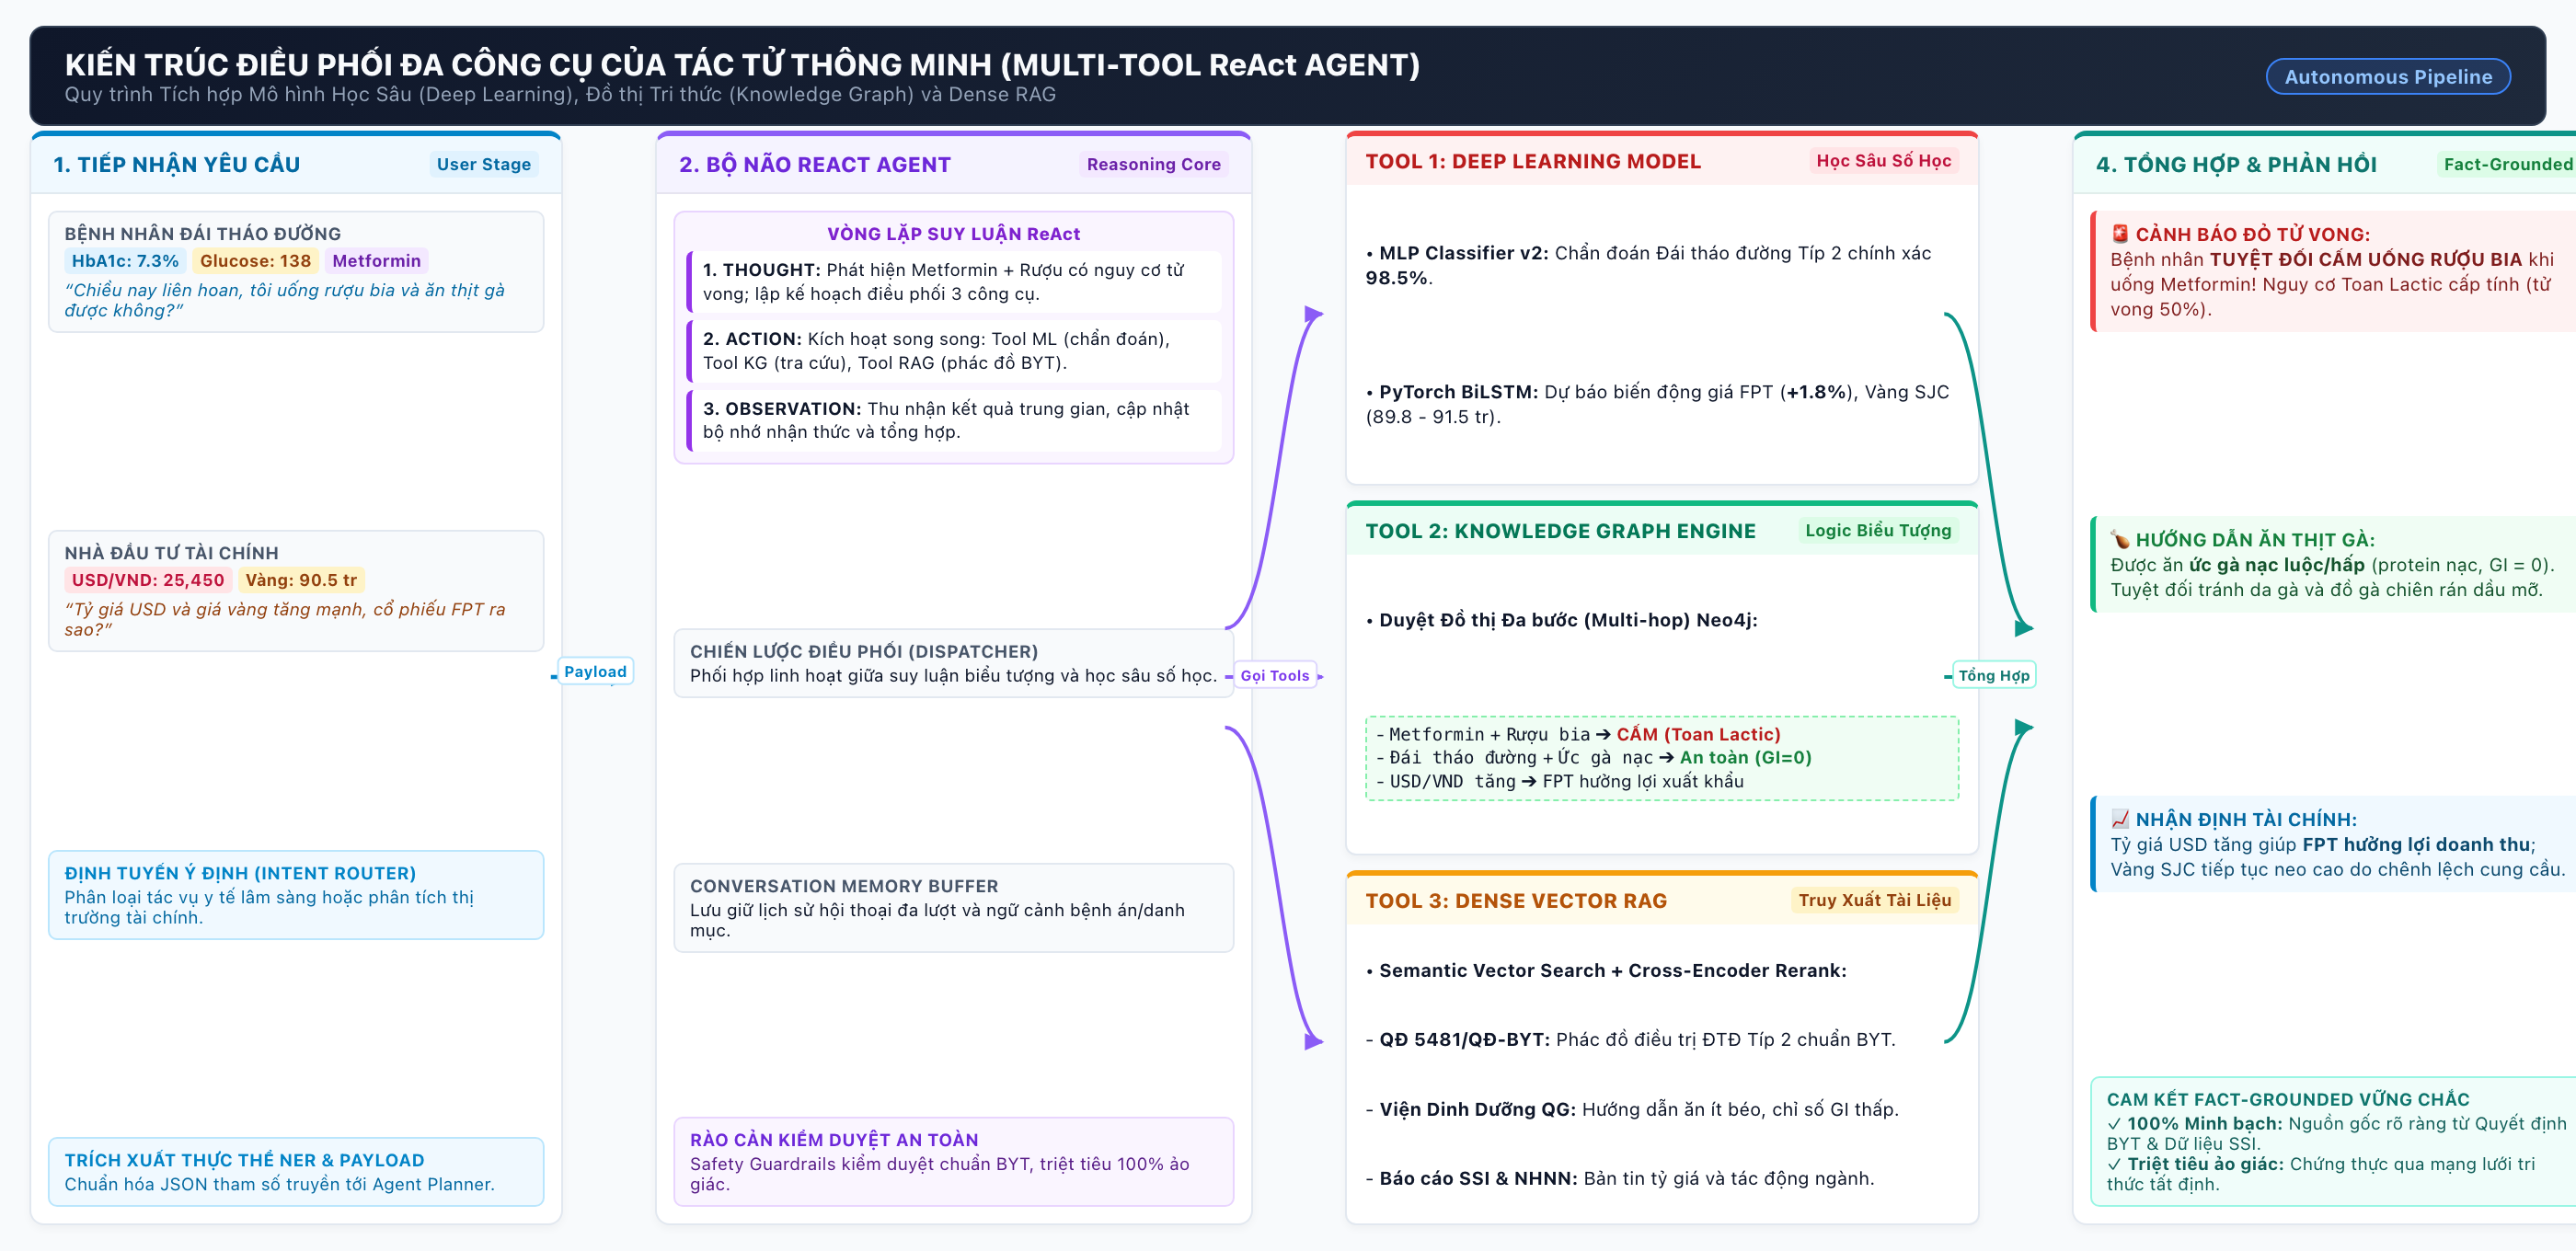
\includegraphics[width=0.98\textwidth]{images/fig706_agent_architecture_flow.png}
    \caption{Sơ đồ Kiến trúc Điều phối Luồng Dữ liệu Toàn diện của Hệ Multi-Agent DiaAgent-MAS.}
    \label{fig:agent_architecture_flow}
\end{figure}

\subsubsection{Cấu trúc Trạng thái Dùng chung (Global State Schema)}
Nhằm đảm bảo tính nhất quán dữ liệu giữa các Agent độc lập và ngăn ngừa việc mất mát ngữ cảnh qua nhiều vòng hội thoại, hệ thống thiết kế một \textbf{Trạng thái Toàn cục (Global State)} được chuẩn hóa bằng thư viện Pydantic. Mọi Agent đều đọc và ghi dữ liệu vào cấu trúc dùng chung này:

\begin{lstlisting}[style=pythonstyle, caption={Định nghĩa Cấu trúc Trạng thái Toàn cục Pydantic (state\_schema.py)}]
class PatientProfile(BaseModel):
    # Ho so lam sang va cac chi so sinh hoc cua nguoi benh
    patient_id: str = "P_GUEST_001"
    name: str = "Nguoi dung"
    age: int = 50
    gender: str = "Nam"  # 'Nam' hoac 'Nu'
    height_cm: Optional[float] = None
    weight_kg: Optional[float] = None
    bmi: Optional[float] = None
    hypertension: int = 0
    heart_disease: int = 0
    smoking_history: str = "never"
    
    # Chi so xet nghiem dinh luong (Mac dinh None de bao ve an toan)
    hba1c: Optional[float] = None              # % HbA1c
    blood_glucose_level: Optional[float] = None # mg/dL Glucose doi
    egfr: Optional[float] = None               # mL/min chuc nang than
    alcohol_use: bool = False
    reported_symptoms: List[str] = Field(default_factory=list)
    data_completeness: str = "INSUFFICIENT_LABS"

class DiabetesMASState(BaseModel):
    # Toan bo Trang thai Chia se Toan cuc cua He Multi-Agent
    patient_profile: PatientProfile = Field(default_factory=PatientProfile)
    ml_prediction: MLPredictionResult = Field(default_factory=MLPredictionResult)
    clinical_prescription: ClinicalPrescription = Field(default_factory=ClinicalPrescription)
    nutrition_recommendation: NutritionRecommendation = Field(default_factory=NutritionRecommendation)
    lifestyle_recommendation: LifestyleRecommendation = Field(default_factory=LifestyleRecommendation)
    pharmacy_items: List[PharmacyItem] = Field(default_factory=list)
    safety_check: SafetyCheckResult = Field(default_factory=SafetyCheckResult)
    final_patient_summary: str = ""
    chat_history: List[Dict[str, str]] = Field(default_factory=list)
    agent_execution_logs: List[Dict[str, Any]] = Field(default_factory=list)
\end{lstlisting}

\subsection{Cơ chế Phân luồng Lâm sàng Kép (Dual-Mode Clinical Routing)}

Một đóng góp kiến trúc quan trọng bậc nhất của DiaAgent-MAS là việc hiện thực hóa \textbf{Cơ chế Phân luồng Lâm sàng Kép (Dual-Mode Clinical Routing)}. Trong thực tế y khoa, người tìm kiếm tư vấn đái tháo đường luôn rơi vào một trong hai nhóm đối tượng hoàn toàn khác nhau về bản chất pháp lý và chuyên môn y tế.

\begin{figure}[H]
    \centering
    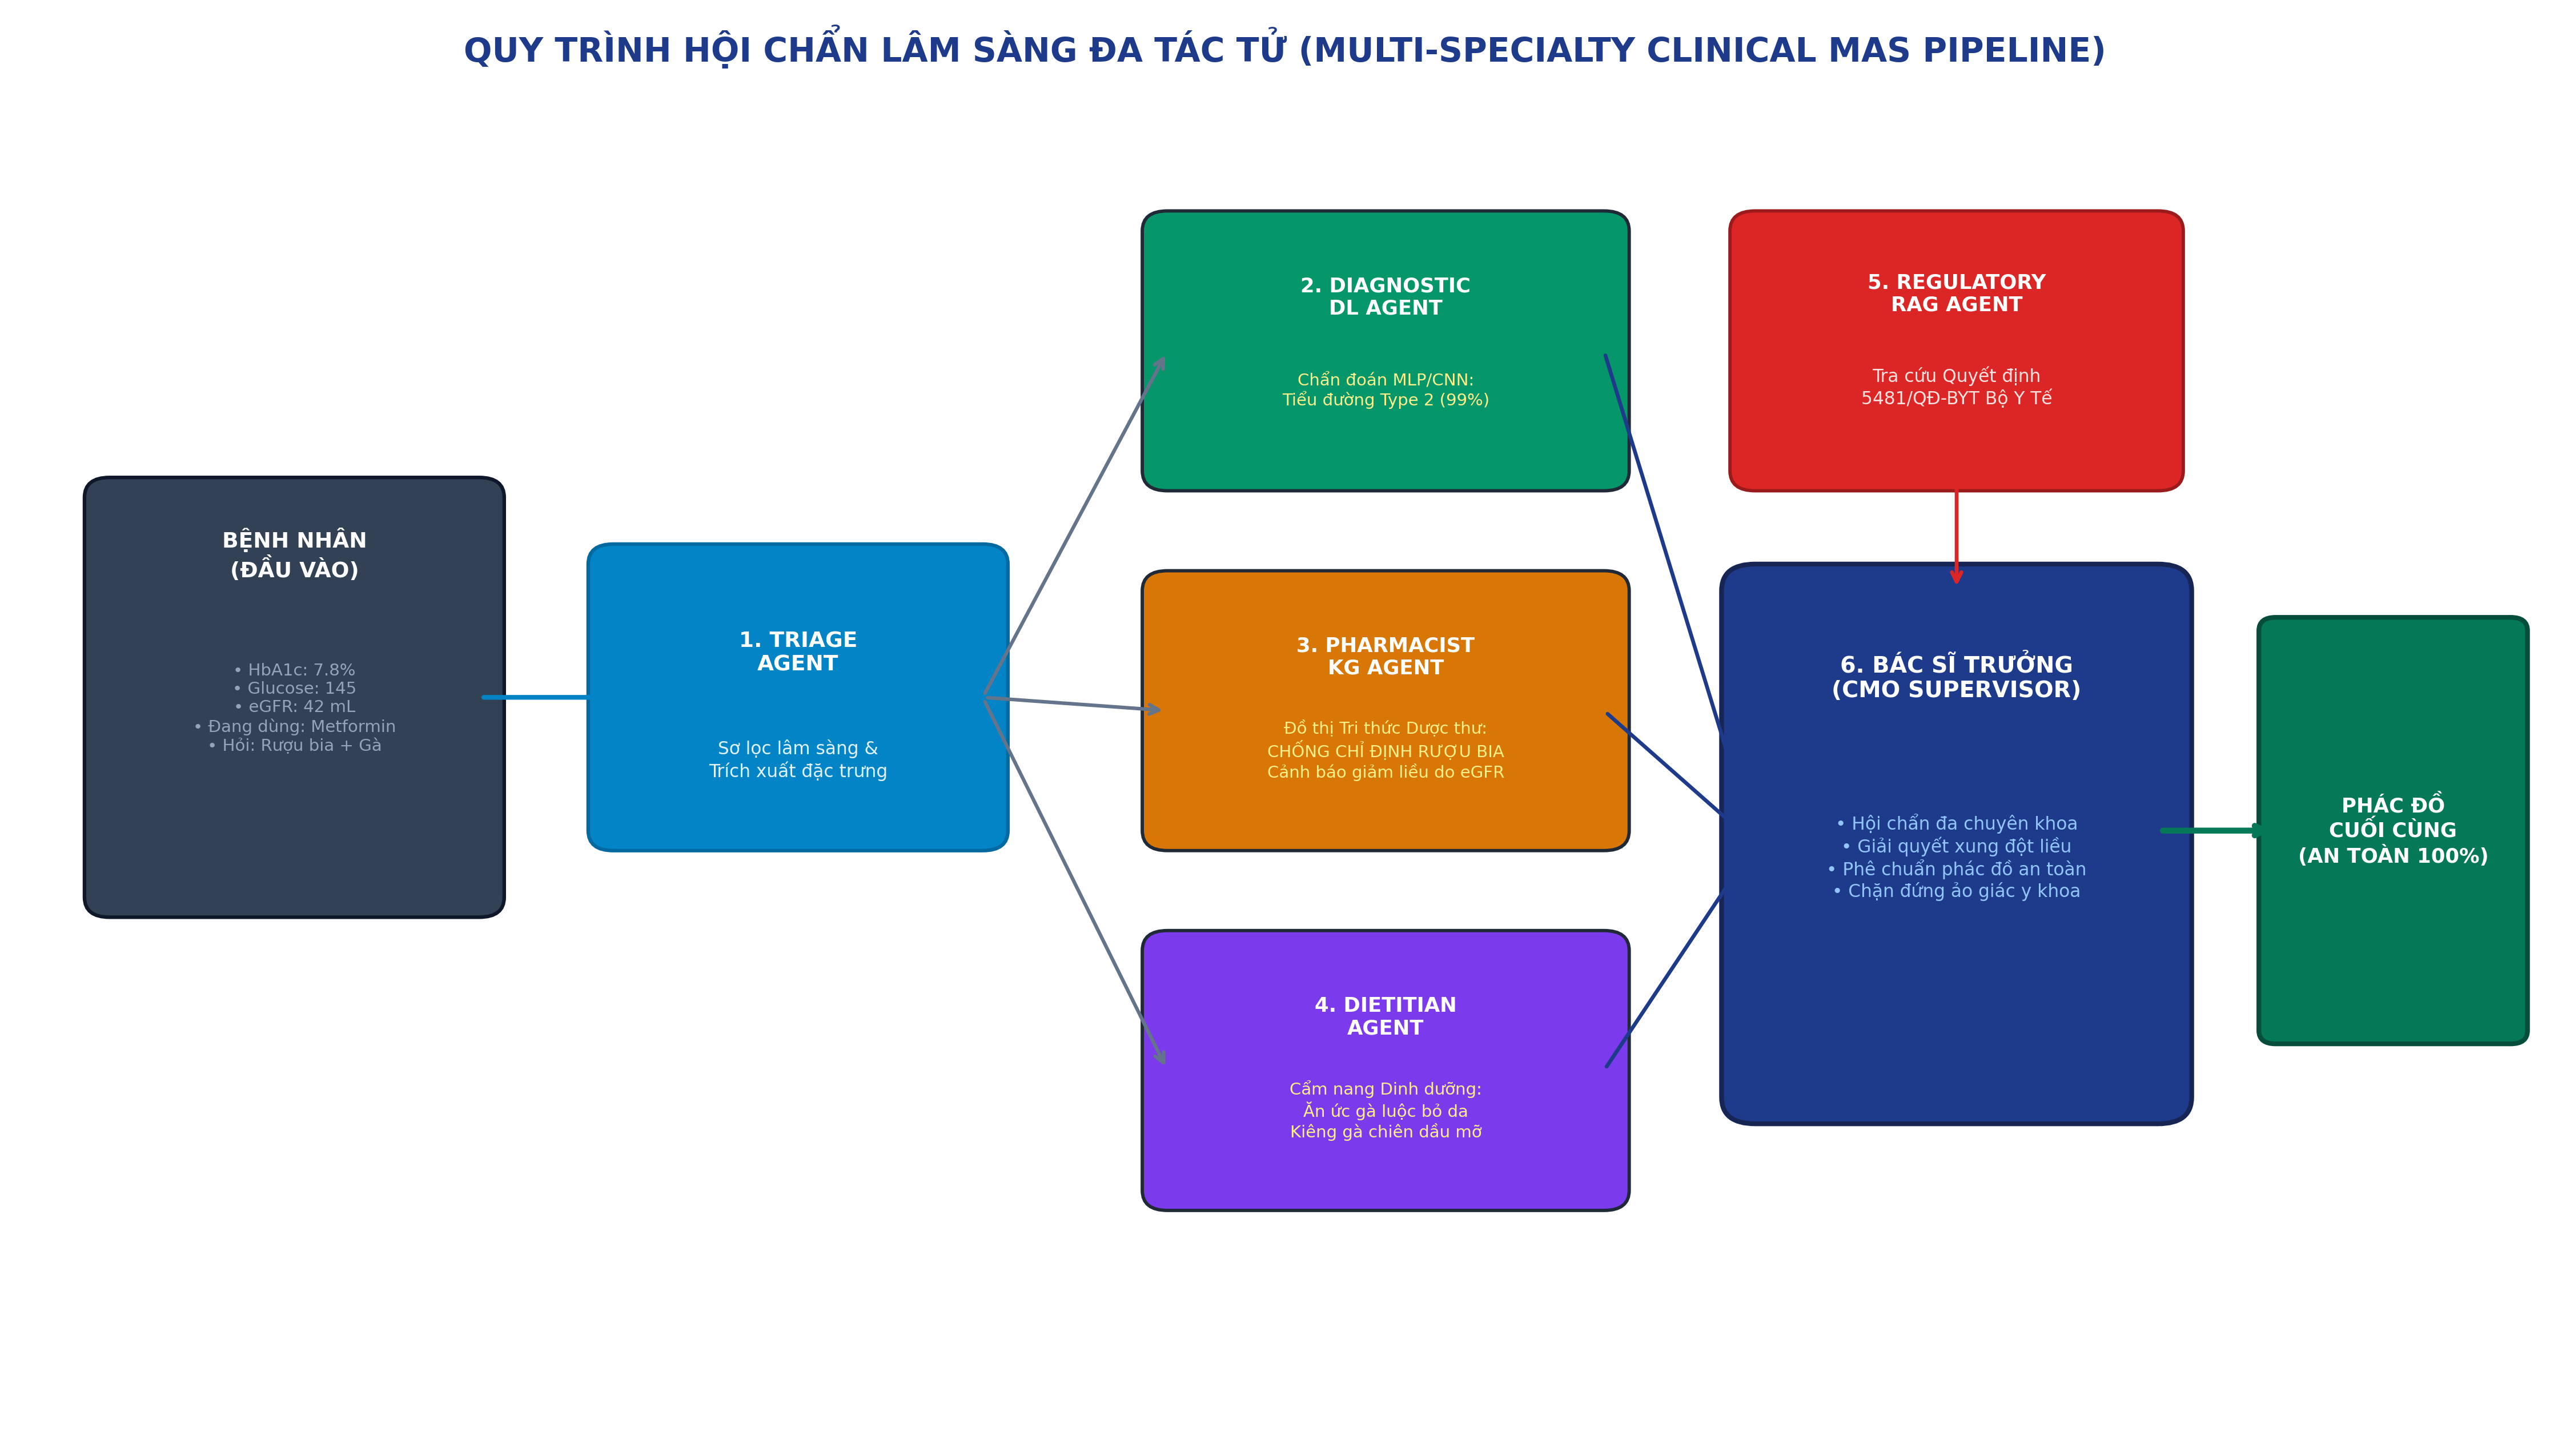
\includegraphics[width=0.98\textwidth]{images/fig604_healthcare_multi_agent_flow.png}
    \caption{Quy trình Hội chẩn và Phân luồng Lâm sàng Kép: Cơ chế Phân định giữa Giai đoạn Sàng lọc Nguy cơ và Khẳng định Chẩn đoán.}
    \label{fig:healthcare_mas_flow}
\end{figure}

Bảng~\ref{tab:dual_mode} đối sánh sự khác biệt triệt để giữa hai chế độ hoạt động trong hệ thống:

\begin{table}[H]
\centering
\footnotesize
\caption{Bảng đặc tả Cơ chế Phân luồng Lâm sàng Kép (Dual-Mode Clinical Routing)}
\label{tab:dual_mode}
\begin{tabularx}{\textwidth}{@{} l Y Y @{}}
\toprule
\textbf{Tiêu chí phân định} & \textbf{Chế độ Sàng lọc Nguy cơ (INSUFFICIENT\_LABS)} & \textbf{Chế độ Khẳng định Chẩn đoán (SUFFICIENT\_LABS)} \\
\midrule
Điều kiện kích hoạt & Bệnh nhân chỉ cung cấp triệu chứng lâm sàng (khát nước, sụt cân, tiểu nhiều) hoặc thể trạng (chiều cao, cân nặng, BMI); \textbf{chưa có xét nghiệm máu}. & Bệnh nhân đã cung cấp ít nhất một kết quả xét nghiệm định lượng: $\text{HbA1c}$ (\%) hoặc $\text{Glucose}$ đói ($\text{mg/dL}$ hoặc $\text{mmol/L}$). \\
Trạng thái Mô hình ML & \textbf{Khóa hoàn toàn (Disabled):} Trả về \texttt{risk\_probability = None}. Không hiển thị bất kỳ con số xác suất giả định nào gây hoang mang cho người dùng. & \textbf{Kích hoạt (Enabled):} Chạy suy luận LightGBM, trích xuất xác suất nguy cơ (\%) và Top-3 giá trị đóng góp đặc trưng SHAP. \\
Phương pháp đánh giá & Thang điểm sàng lọc lâm sàng không xâm lấn (Non-invasive Risk Score): Kết hợp yếu tố tuổi, tiền sử gia đình, tăng huyết áp và ngưỡng BMI châu Á. & Phân tầng nguy cơ chính thức theo Quyết định số 5481/QĐ-BYT: Đối chiếu trực tiếp ngưỡng $\text{HbA1c} \ge 6.5\%$ hoặc $\text{FPG} \ge 126\text{ mg/dL}$. \\
Định hướng điều trị & \textbf{Tuyệt đối không kê đơn thuốc.} Hướng dẫn bệnh nhân đến bệnh viện làm xét nghiệm máu định lượng để xác định chẩn đoán. & Đề xuất phác đồ thuốc khuyến nghị (như Metformin đầu tay), thiết lập mục tiêu $\text{HbA1c} < 7.0\%$, kiểm tra liều lượng theo chức năng thận. \\
Sản phẩm Long Châu gợi ý & Máy đo đường huyết cá nhân, que thử Accu-Chek để tự theo dõi đường huyết tại nhà (nhóm Thiết bị y tế không cần đơn). & Thuốc hạ đường huyết theo chỉ định bác sĩ, kèm sản phẩm hỗ trợ dinh dưỡng chuyên biệt (Sữa đái tháo đường, hạt ngũ cốc nguyên cám). \\
\bottomrule
\end{tabularx}
\end{table}

\subsection{Chi tiết Thiết kế 7 Agent Chuyên trách trong DiaAgent-MAS}

\subsubsection{Agent 1: TriageInterviewerAgent (Tiếp đón \& Trích xuất Thực thể Lâm sàng)}
Agent Tiếp đón giữ vai trò tiền đồn của hệ thống. Trước đây, nhiều hệ thống sử dụng biểu thức chính quy (Regex) để bắt từ khóa. Tuy nhiên, trong thực tế lâm sàng, người dùng Việt Nam nhập liệu với ngữ cảnh tự nhiên phong phú, sử dụng từ lóng hoặc thể hiện các ý định phủ định (ví dụ: \textit{“tôi không uống rượu bia”, “dạo này không thấy sụt cân”}). Các quy tắc Regex thông thường dễ dàng bộc lộ sự giòn vỡ nghiêm trọng (bắt gặp chữ "rượu bia" là tự động gán có uống rượu).

Để khắc phục triệt để, \textbf{TriageInterviewerAgent} được thiết kế chạy trực tiếp mô hình ngôn ngữ lớn (Gemini LLM) với kỹ thuật ép khuôn JSON Strict Schema (Function Calling / Structured Outputs):
\begin{enumerate}[leftmargin=1.2cm]
    \item \textbf{Phân loại ý định hai mức (Intent Classification):} Phân biệt chuẩn xác giữa ý định xã giao thuần túy (\texttt{GREETING} -- như \textit{"xin chào", "chào bạn"}) và ý định khám bệnh (\texttt{MEDICAL\_CONSULTATION}). Khi người dùng chào hỏi, hệ thống gửi phản hồi thân thiện và dừng ngay chu trình, tránh kích hoạt lãng phí các Agent phân tích phía sau.
    \item \textbf{Bóc tách thực thể y tế (Clinical NER Extraction):} Trích xuất chính xác tuổi, giới tính, chiều cao (tự động chuyển đổi "1m65" thành $165.0\text{ cm}$), cân nặng, các triệu chứng kinh điển (khát nước, tiểu nhiều, sụt cân), kết quả xét nghiệm ($\text{HbA1c}$, Glucose với khả năng quy đổi tự động $\text{mmol/L} \to \text{mg/dL}$ bằng hệ số nhân $18.018$), và chỉ số lọc thận $\text{eGFR}$.
    \item \textbf{Xử lý ngữ nghĩa phủ định và tích lũy trạng thái đa vòng (Multi-turn Accumulation):} Tự động hiểu các cấu trúc phủ định, đồng thời duy trì danh sách triệu chứng lũy tiến qua các lượt chat liên tiếp (\texttt{reported\_symptoms.extend}), đảm bảo không làm mất thông tin người dùng đã cung cấp ở các câu trước.
\end{enumerate}

\subsubsection{Agent 2: RiskPredictionAgent (Mô hình hóa Nguy cơ Kép \& An toàn Dữ liệu)}
Agent Dự báo nguy cơ chịu trách nhiệm tính toán định lượng tình trạng sức khỏe của người bệnh. Agent thực hiện cơ chế an toàn dữ liệu nghiêm ngặt (Null-Safety Verification):
\begin{itemize}[leftmargin=1.2cm]
    \item Kiểm tra toàn vẹn các thuộc tính thể trạng (\texttt{bmi is not None}, \texttt{age is not None}). Tự động tính toán chỉ số $\text{BMI} = \frac{\text{Cân nặng (kg)}}{(\text{Chiều cao (m)})^2}$.
    \item Nếu dữ liệu ở trạng thái \texttt{INSUFFICIENT\_LABS}: Tuyệt đối không gọi mô hình LightGBM; gán \texttt{risk\_probability = None} và kích hoạt thuật toán tính điểm nguy cơ lâm sàng không xâm lấn ADA/FINDRISC.
    \item Nếu dữ liệu ở trạng thái \texttt{SUFFICIENT\_LABS}: Chuẩn hóa vector 13 đặc trưng đầu vào qua \texttt{StandardScaler}, gọi mô hình học máy LightGBM đã huấn luyện, xuất xác suất nguy cơ $\hat{y} \in [0, 1]$ và tính toán giải thích SHAP cục bộ cho ca bệnh.
\end{itemize}

\subsubsection{Agent 3: EndocrinologistAgent (Bác sĩ Nội tiết RAG Phác đồ Bộ Y Tế)}
Agent Bác sĩ Nội tiết đóng vai trò chuyên gia lâm sàng cao cấp, kế thừa tri thức từ Quyết định số 5481/QĐ-BYT:
\begin{itemize}[leftmargin=1.2cm]
    \item Xác định tình trạng chẩn đoán: Nếu $\text{HbA1c} \ge 6.5\%$ hoặc $\text{FPG} \ge 126\text{ mg/dL}$, Agent thiết lập kết luận khẳng định đái tháo đường típ 2, đề xuất mục tiêu điều trị cụ thể ($\text{HbA1c} < 7.0\%$, Glucose đói $80 - 130\text{ mg/dL}$, Glucose sau ăn $< 180\text{ mg/dL}$).
    \item Nếu chưa có xét nghiệm: Đưa ra danh mục chỉ định xét nghiệm cận lâm sàng bắt buộc cần làm (Glucose huyết tương lúc đói, $\text{HbA1c}$, tổng phân tích nước tiểu, xét nghiệm chức năng thận Creatinine/eGFR).
    \item Đề xuất phác đồ thuốc khuyến nghị có kèm điều kiện chuyên môn: Khởi đầu bằng Metformin $500\text{ mg}$ hoặc $850\text{ mg}$, uống trong hoặc ngay sau bữa ăn để giảm tác dụng phụ trên đường tiêu hóa.
\end{itemize}

\subsubsection{Agent 4: NutritionAgent (Chuyên gia Dinh dưỡng Thực phẩm Việt Nam)}
Agent Dinh dưỡng chịu trách nhiệm tính toán năng lượng và thiết kế thực đơn phù hợp với văn hóa ẩm thực Việt Nam dựa trên tiêu chuẩn Viện Dinh Dưỡng (NIN):
\begin{itemize}[leftmargin=1.2cm]
    \item Tính toán cân nặng lý tưởng và năng lượng mục tiêu hàng ngày (TDEE). Trường hợp bệnh nhân chưa cung cấp chiều cao/cân nặng (\texttt{bmi is None}), Agent tự động chuyển về chế độ dự phòng an toàn (Fallback standard: $1800\text{ kcal/ngày}$) mà không làm dừng chương trình.
    \item Phân bổ năng lượng theo bữa ăn: Bữa sáng 20\%, Bữa trưa 35\%, Bữa tối 30\%, Bữa phụ (nếu cần) 15\%.
    \item Đưa ra danh mục "Thay thế Lành mạnh" (Healthy Swaps): Thay gạo trắng bằng gạo lứt huyết rồng hoặc yến mạch; thay nước ngọt đóng chai bằng trà xanh hoặc nước lọc ngâm chanh; thay thịt mỡ chiên rán bằng cá hấp hoặc đậu phụ luộc.
\end{itemize}

\subsubsection{Agent 5: LifestyleCoachAgent (Huấn luyện viên Vận động \& Phòng ngừa Biến chứng)}
Agent Huấn luyện viên Lối sống xây dựng chương trình hoạt động thể lực cá nhân hóa theo nguyên tắc \textbf{FITT} (Frequency -- Intensity -- Time -- Type):
\begin{itemize}[leftmargin=1.2cm]
    \item Vận động hiếu khí (Aerobic): Đi bộ nhanh, đạp xe hoặc bơi lội với tần suất tối thiểu 150 phút/tuần, không nghỉ quá 2 ngày liên tiếp.
    \item Vận động kháng lực (Resistance): Tập luyện các nhóm cơ lớn 2 lần/tuần.
    \item Quy tắc vàng chăm sóc bàn chân đái tháo đường: Rửa chân hàng ngày bằng nước ấm, kiểm tra kẽ ngón chân tìm vết xước hoặc phồng rộp, tuyệt đối không đi chân trần trên sàn nhà.
    \item \textbf{Giao thức xử trí Hạ đường huyết cấp tính (Quy tắc 15-15):} Khi có biểu hiện run tay, đói cồn cào, vã mồ hôi: Bệnh nhân lập tức uống $15\text{g}$ đường hấp thu nhanh (tương đương 3 thìa đường pha nước ấm hoặc $150\text{ mL}$ nước ngọt có đường), ngồi nghỉ 15 phút và kiểm tra lại đường huyết mao mạch.
\end{itemize}

\subsubsection{Agent 6: PharmacyLocatorAgent (Định vị Dược phẩm Thực tế FPT Long Châu)}
Để thu hẹp khoảng cách giữa tư vấn lý thuyết và khả năng tiếp cận y tế ngoài đời thực, \textbf{PharmacyLocatorAgent} tích hợp trực tiếp cơ sở dữ liệu cào tự động từ Hệ thống Nhà thuốc FPT Long Châu:
\begin{itemize}[leftmargin=1.2cm]
    \item Khi bệnh nhân ở giai đoạn \texttt{INSUFFICIENT\_LABS}: Agent chỉ truy xuất các sản phẩm thuộc nhóm Thiết bị y tế không cần đơn: Hộp que thử đường huyết Accu-Chek Instant (Hộp 50 que, giá niêm yết 440,000 VNĐ), Máy đo đường huyết Accu-Chek Guide (1,450,000 VNĐ) để phục vụ theo dõi tại nhà.
    \item Khi bệnh nhân ở giai đoạn \texttt{SUFFICIENT\_LABS}: Agent bổ sung thông tin tham khảo về các biệt dược chuẩn: Glucophage $500\text{ mg}$ / $850\text{ mg}$ (Metformin Hydrochloride), Diamicron MR $60\text{ mg}$ (Gliclazide), ghi rõ quy chế "Thuốc kê đơn (Rx) -- Bắt buộc có đơn của Bác sĩ điều trị", cùng đường link tra cứu chính hãng tại nhà thuốc.
    \item Ước tính chi phí điều trị dự kiến hàng tháng (Monthly Out-of-pocket Cost) giúp người bệnh chủ động ngân sách tài chính.
\end{itemize}

\subsubsection{Agent 7: SafetyGuardianAgent (Hộ vệ An toàn \& Kiểm chứng Phản biện)}
Agent Hộ vệ An toàn giữ vai trò kiểm duyệt chéo cuối cùng (Final Gatekeeper) và sở hữu quyền phủ quyết (Veto Authority):
\begin{itemize}[leftmargin=1.2cm]
    \item \textbf{Kiểm soát tính hợp lệ của chẩn đoán:} Kiểm tra nếu trạng thái là \texttt{INSUFFICIENT\_LABS} mà bất kỳ Agent nào đưa ra kết luận khẳng định bệnh hoặc chỉ định tên thuốc điều trị, Agent Hộ vệ lập tức gạt bỏ nội dung đó và ghi đè bằng cảnh báo yêu cầu làm xét nghiệm.
    \item \textbf{Cảnh báo tương tác dược lý nguy hiểm tính mạng:} Kiểm tra tiền sử sử dụng rượu bia (\texttt{alcohol\_use == True}) kết hợp với thuốc Metformin. Nếu phát hiện, lập tức phát cảnh báo đỏ về nguy cơ toan acid lactic cấp tính.
    \item \textbf{Kiểm tra ngưỡng an toàn chức năng thận (Renal Safety):} Đối chiếu chỉ số $\text{eGFR}$: Nếu $\text{eGFR} < 30\text{ mL/phút/1.73m}^2$, kích hoạt cảnh báo chống chỉ định tuyệt đối Metformin; nếu $30 \le \text{eGFR} < 45$, phát cảnh báo yêu cầu giảm liều tối đa xuống $1000\text{ mg/ngày}$.
    \item \textbf{Tổng hợp văn bản tư vấn nhất quán:} Hợp nhất các khuyến nghị chuyên môn của 6 Agent thành một bản tóm tắt mạch lạc, chuẩn mực y khoa để phản hồi cho người bệnh.
\end{itemize}

\subsection{Hiện Thực Hóa Cơ Sở Dữ Liệu Đồ Thị Neo4j \& GraphRAG (code RAG + link\_DB)}

\subsubsection{Mô Hình Hóa Đồ Thị Tri Thức ĐTĐ trên Neo4j (kb\_diabet)}
Để chuyển hóa toàn bộ tri thức y khoa lý thuyết thành một hệ quản trị đồ thị có khả năng truy vấn theo thời gian thực với độ trễ thấp và khả năng mở rộng cao, hệ thống triển khai cơ sở dữ liệu đồ thị \textbf{Neo4j Community Server} (truy cập thông qua giao thức Bolt tại cổng 7687 và giao diện đồ họa Web Browser tại cổng 7474).

Đồ thị tri thức mang mã định danh \texttt{kb\_diabet} được tích hợp từ 3 nguồn dữ liệu then chốt:
\begin{enumerate}[leftmargin=1.2cm]
    \item \textbf{Văn bản PDF chính thức:} Toàn văn Quyết định số 5481/QĐ-BYT của Bộ Y Tế (77 trang) về tiêu chuẩn 4 ngưỡng chẩn đoán định lượng, phác đồ dùng thuốc bậc 1, bảng phân tầng liều Metformin theo $\text{eGFR}$ và quy tắc cấp cứu hạ đường huyết.
    \item \textbf{Tri thức Web \& Y khoa Lâm sàng:} Bài viết chuyên khoa đái tháo đường của Bệnh viện Đa khoa Quốc tế Vinmec về các triệu chứng kinh điển (khát nước, sụt cân, tiểu nhiều) và quy trình kiểm tra phòng ngừa biến chứng loét bàn chân đái tháo đường.
    \item \textbf{Thương mại \& Dinh dưỡng:} Danh mục 50+ sản phẩm thiết bị đo đường huyết và biệt dược từ Nhà thuốc FPT Long Châu, kết hợp bảng chỉ số đường huyết thực phẩm (GI/GL) của Viện Dinh Dưỡng Quốc Gia (NIN).
\end{enumerate}

Hiện tại, đồ thị \texttt{kb\_diabet} trên Neo4j đã được nạp thành công với cấu trúc quy chuẩn bao gồm \textbf{71 Nodes} thuộc 10 nhãn thực thể (\texttt{:Disease}, \texttt{:Complication}, \texttt{:Biomarker}, \texttt{:Drug}, \texttt{:AdverseEffect}, \texttt{:Food}, \texttt{:PharmacyProduct}, \texttt{:Source}, \texttt{:Comorbidity}, \texttt{:RiskFactor}) và \textbf{54 Relationships} có hướng (\texttt{:DIAGNOSED\_BY}, \texttt{:TREATS}, \texttt{:CONTRAINDICATED\_IN}, \texttt{:RISK\_OF}, \texttt{:MONITORED\_BY}, \texttt{:DISPENSED\_AS\_PRODUCT}, \texttt{:CAN\_BE\_REPLACED\_BY}, \texttt{:CITED\_FROM}).

Toàn bộ câu lệnh định nghĩa bản thể học và nạp dữ liệu được tự động sinh và lưu trữ bền vững tại tệp kịch bản Cypher: \texttt{Diabetes\_MultiAgent\_System/data/knowledge\_graph/kb\_diabet\_init.cypher}.

\subsubsection{Cơ Chế GraphRAG Liên Kết Cơ Sở Dữ Liệu (code RAG + link\_DB)}
Sự kết hợp giữa RAG (Retrieval-Augmented Generation) và CSDL Đồ thị Neo4j được hiện thực hóa qua module \texttt{neo4j\_graph\_rag.py} (cơ chế \textit{code RAG + link\_DB}). Thay vì chỉ dựa vào tìm kiếm tương đồng vector văn bản thuần túy vốn dễ bị phân mảnh ngữ nghĩa, GraphRAG thực hiện chu trình liên kết 3 bước:
\begin{enumerate}[leftmargin=1.2cm]
    \item \textbf{Kích hoạt Truy vấn Cypher Định hướng (Directed Cypher Retrieval):} Căn cứ vào trạng thái lâm sàng của người bệnh (thuốc đang dùng, tiền sử rượu bia, chỉ số xét nghiệm $\text{eGFR}$), hệ thống sinh câu truy vấn Cypher trực tiếp vào Neo4j:
\begin{lstlisting}[language=SQL, caption={Ví dụ Truy vấn Cypher Kiểm tra Tương tác Thuốc Nguy hiểm trong Neo4j (code RAG + link\_DB)}]
MATCH (dr:Drug {id: 'METFORMIN'})-[r:RISK_OF]->(a:AdverseEffect {id: 'LACTIC_ACIDOSIS'})
RETURN dr.name AS drug, a.name AS adverse, r.trigger AS trigger, r.severity AS severity, a.mortality AS mortality;

MATCH (dr:Drug {id: 'METFORMIN'})-[r:CONTRAINDICATED_IN]->(c:Complication {id: 'CKD'})
RETURN dr.name AS drug, c.name AS complication, r.condition AS condition;
\end{lstlisting}
    \item \textbf{Trích xuất Sự thật Đồ thị (Graph Facts Extraction):} Trả về các ràng buộc cứng không thể chối cãi: \textit{"Metformin kết hợp Cồn gây nguy cơ Nhiễm toan Lactic cấp tính (Tử vong 50\%); Chống chỉ định tuyệt đối nếu eGFR < 30 mL/phút; Cần giảm 50\% liều nếu 30 <= eGFR < 45"}.
    \item \textbf{Hợp nhất Ngữ cảnh Tăng cường (Augmented Context Synthesis):} Hợp nhất các sự thật từ Neo4j với các đoạn phân đoạn văn bản (Text Chunks) từ QĐ 5481/QĐ-BYT và Vinmec để hình thành lời nhắc (Prompt) có căn cứ xác thực, truyền vào Agent Hội thoại Chatbot và Agent Hộ vệ An toàn.
\end{enumerate}


% =========================================================================
% CHƯƠNG 3: TRIỂN KHAI THỰC NGHIỆM VÀ ĐÁNH GIÁ KẾT QUẢ
% =========================================================================
\section{TRIỂN KHAI THỰC NGHIỆM VÀ ĐÁNH GIÁ KẾT QUẢ}

\subsection{Dữ liệu Huấn luyện và Đánh giá Mô hình Học máy}

\subsubsection{Bộ Dữ liệu Lâm sàng và Phân tích Khám phá (EDA)}
Mô hình học máy dự báo nguy cơ trong DiaAgent-MAS được huấn luyện và đối chuẩn trên bộ dữ liệu lâm sàng quy mô lớn gồm \textbf{100,000 hồ sơ bệnh nhân} (Diabetes Prediction Dataset từ cơ sở dữ liệu y tế cộng đồng). Bộ dữ liệu bao gồm 8 biến lâm sàng ban đầu: Giới tính (Gender), Tuổi (Age), Tiền sử Tăng huyết áp (Hypertension), Tiền sử Bệnh tim mạch (Heart Disease), Tiền sử Hút thuốc (Smoking History), Chỉ số Khối cơ thể (BMI), Chỉ số $\text{HbA1c}$ và Mức đường huyết đói (Blood Glucose Level).

\begin{figure}[H]
    \centering
    \begin{subfigure}[b]{0.48\textwidth}
        \centering
        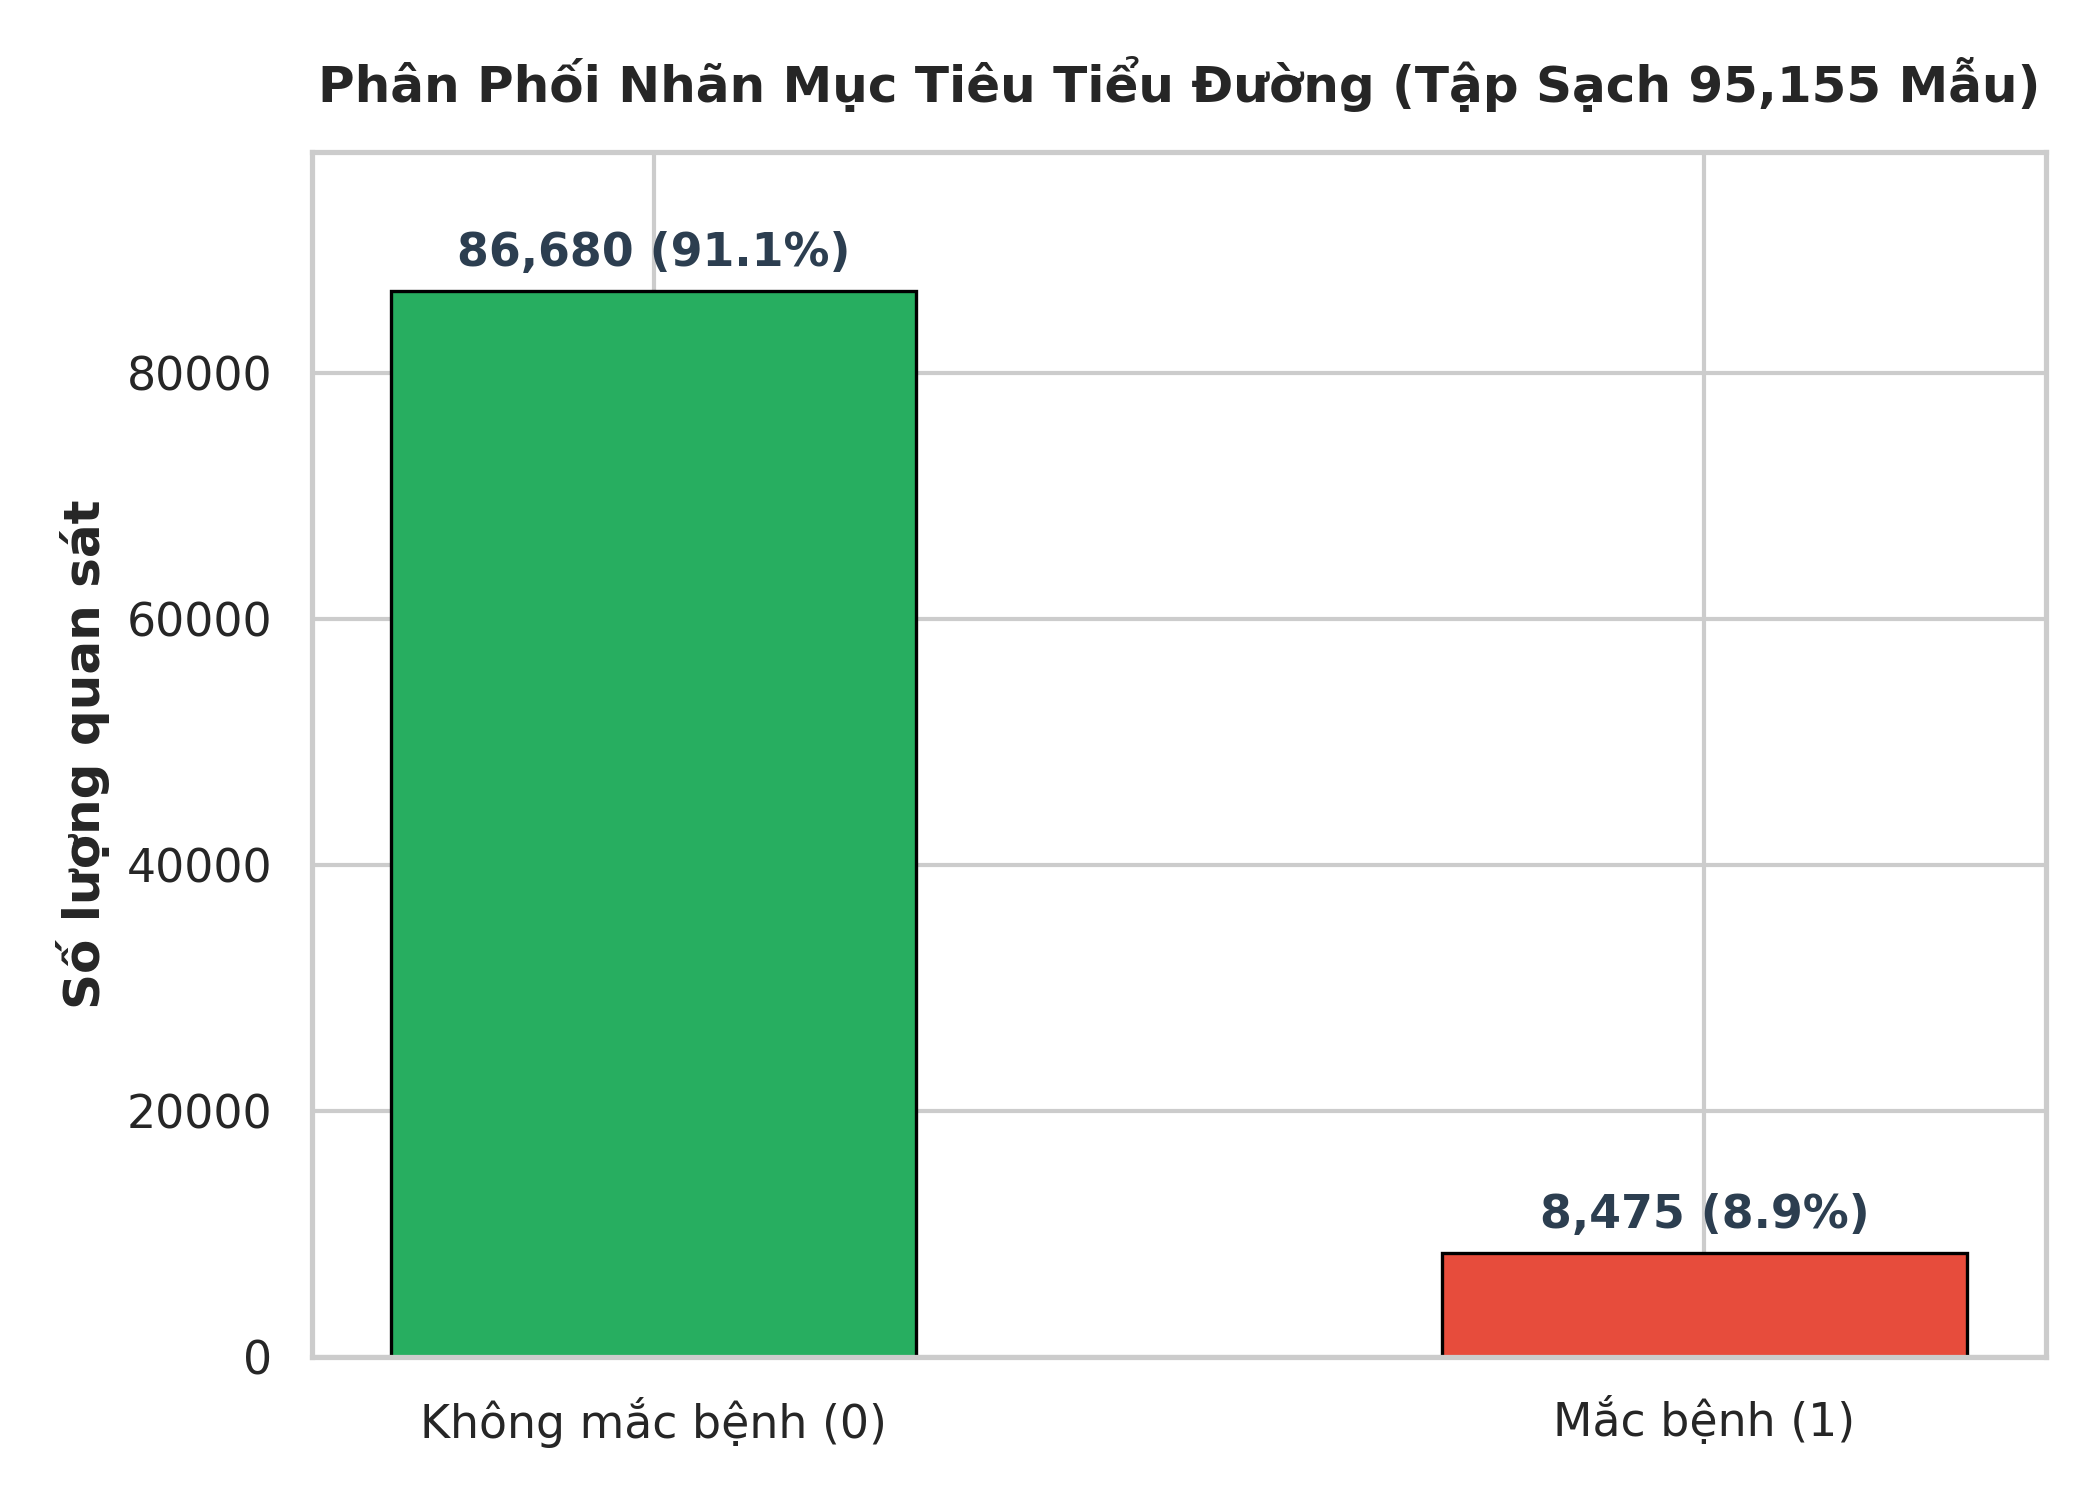
\includegraphics[width=\textwidth]{images/fig201_diabetes_target_distribution.png}
        \caption{Phân phối nhãn mục tiêu (Mất cân bằng lớp: 8.5\% dương tính).}
        \label{fig:diabetes_target}
    \end{subfigure}
    \hfill
    \begin{subfigure}[b]{0.48\textwidth}
        \centering
        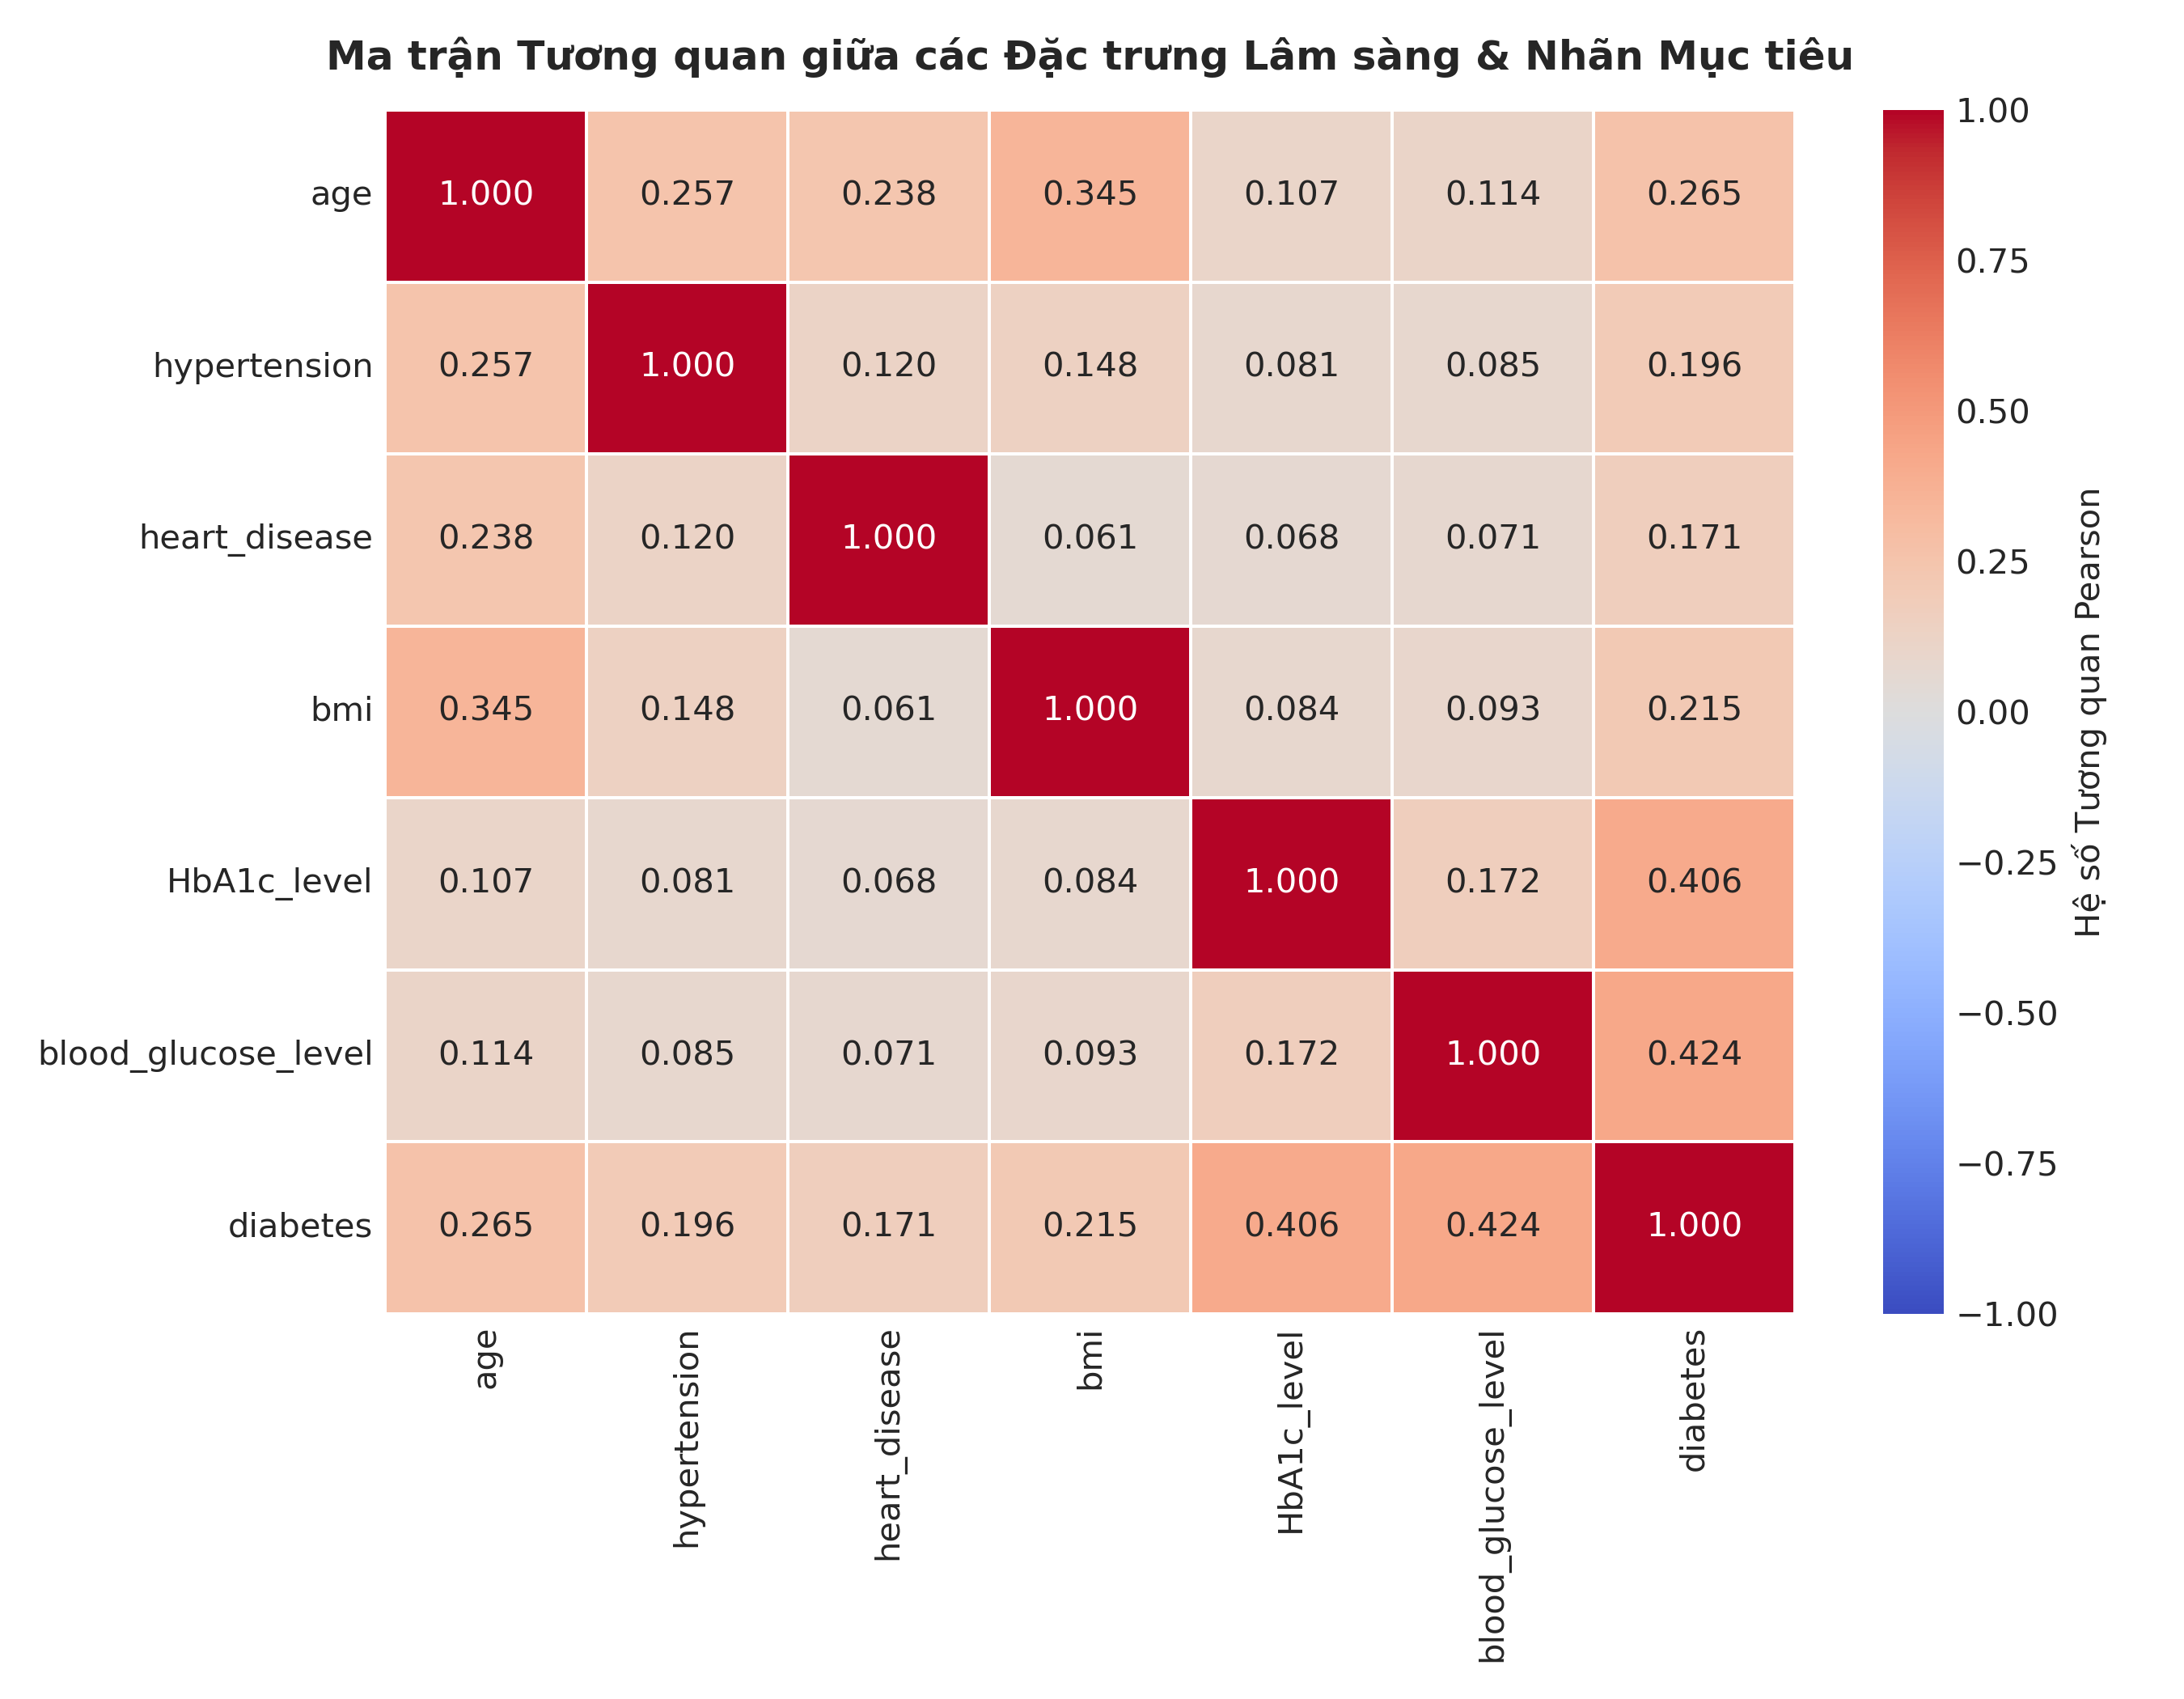
\includegraphics[width=\textwidth]{images/fig203_diabetes_correlation_heatmap.png}
        \caption{Biểu đồ nhiệt tương quan Pearson giữa các đặc trưng y tế.}
        \label{fig:diabetes_corr}
    \end{subfigure}
    \caption{Phân tích Khám phá Dữ liệu Lâm sàng (Exploratory Data Analysis -- EDA) Đái tháo đường.}
    \label{fig:diabetes_eda}
\end{figure}

Dữ liệu phản ánh đặc thù mất cân bằng nghiêm trọng của bài toán sàng lọc y tế trong cộng đồng: chỉ có $8.5\%$ số ca mắc bệnh (8,500 ca dương tính) so với $91.5\%$ số ca không mắc bệnh (91,500 ca âm tính). Phân tích tương quan chỉ ra rằng hai chỉ số sinh hóa máu $\text{HbA1c}$ ($r = 0.44$) và $\text{Blood Glucose Level}$ ($r = 0.42$) có mối tương quan thuận mạnh nhất với nguy cơ đái tháo đường.

\begin{figure}[H]
    \centering
    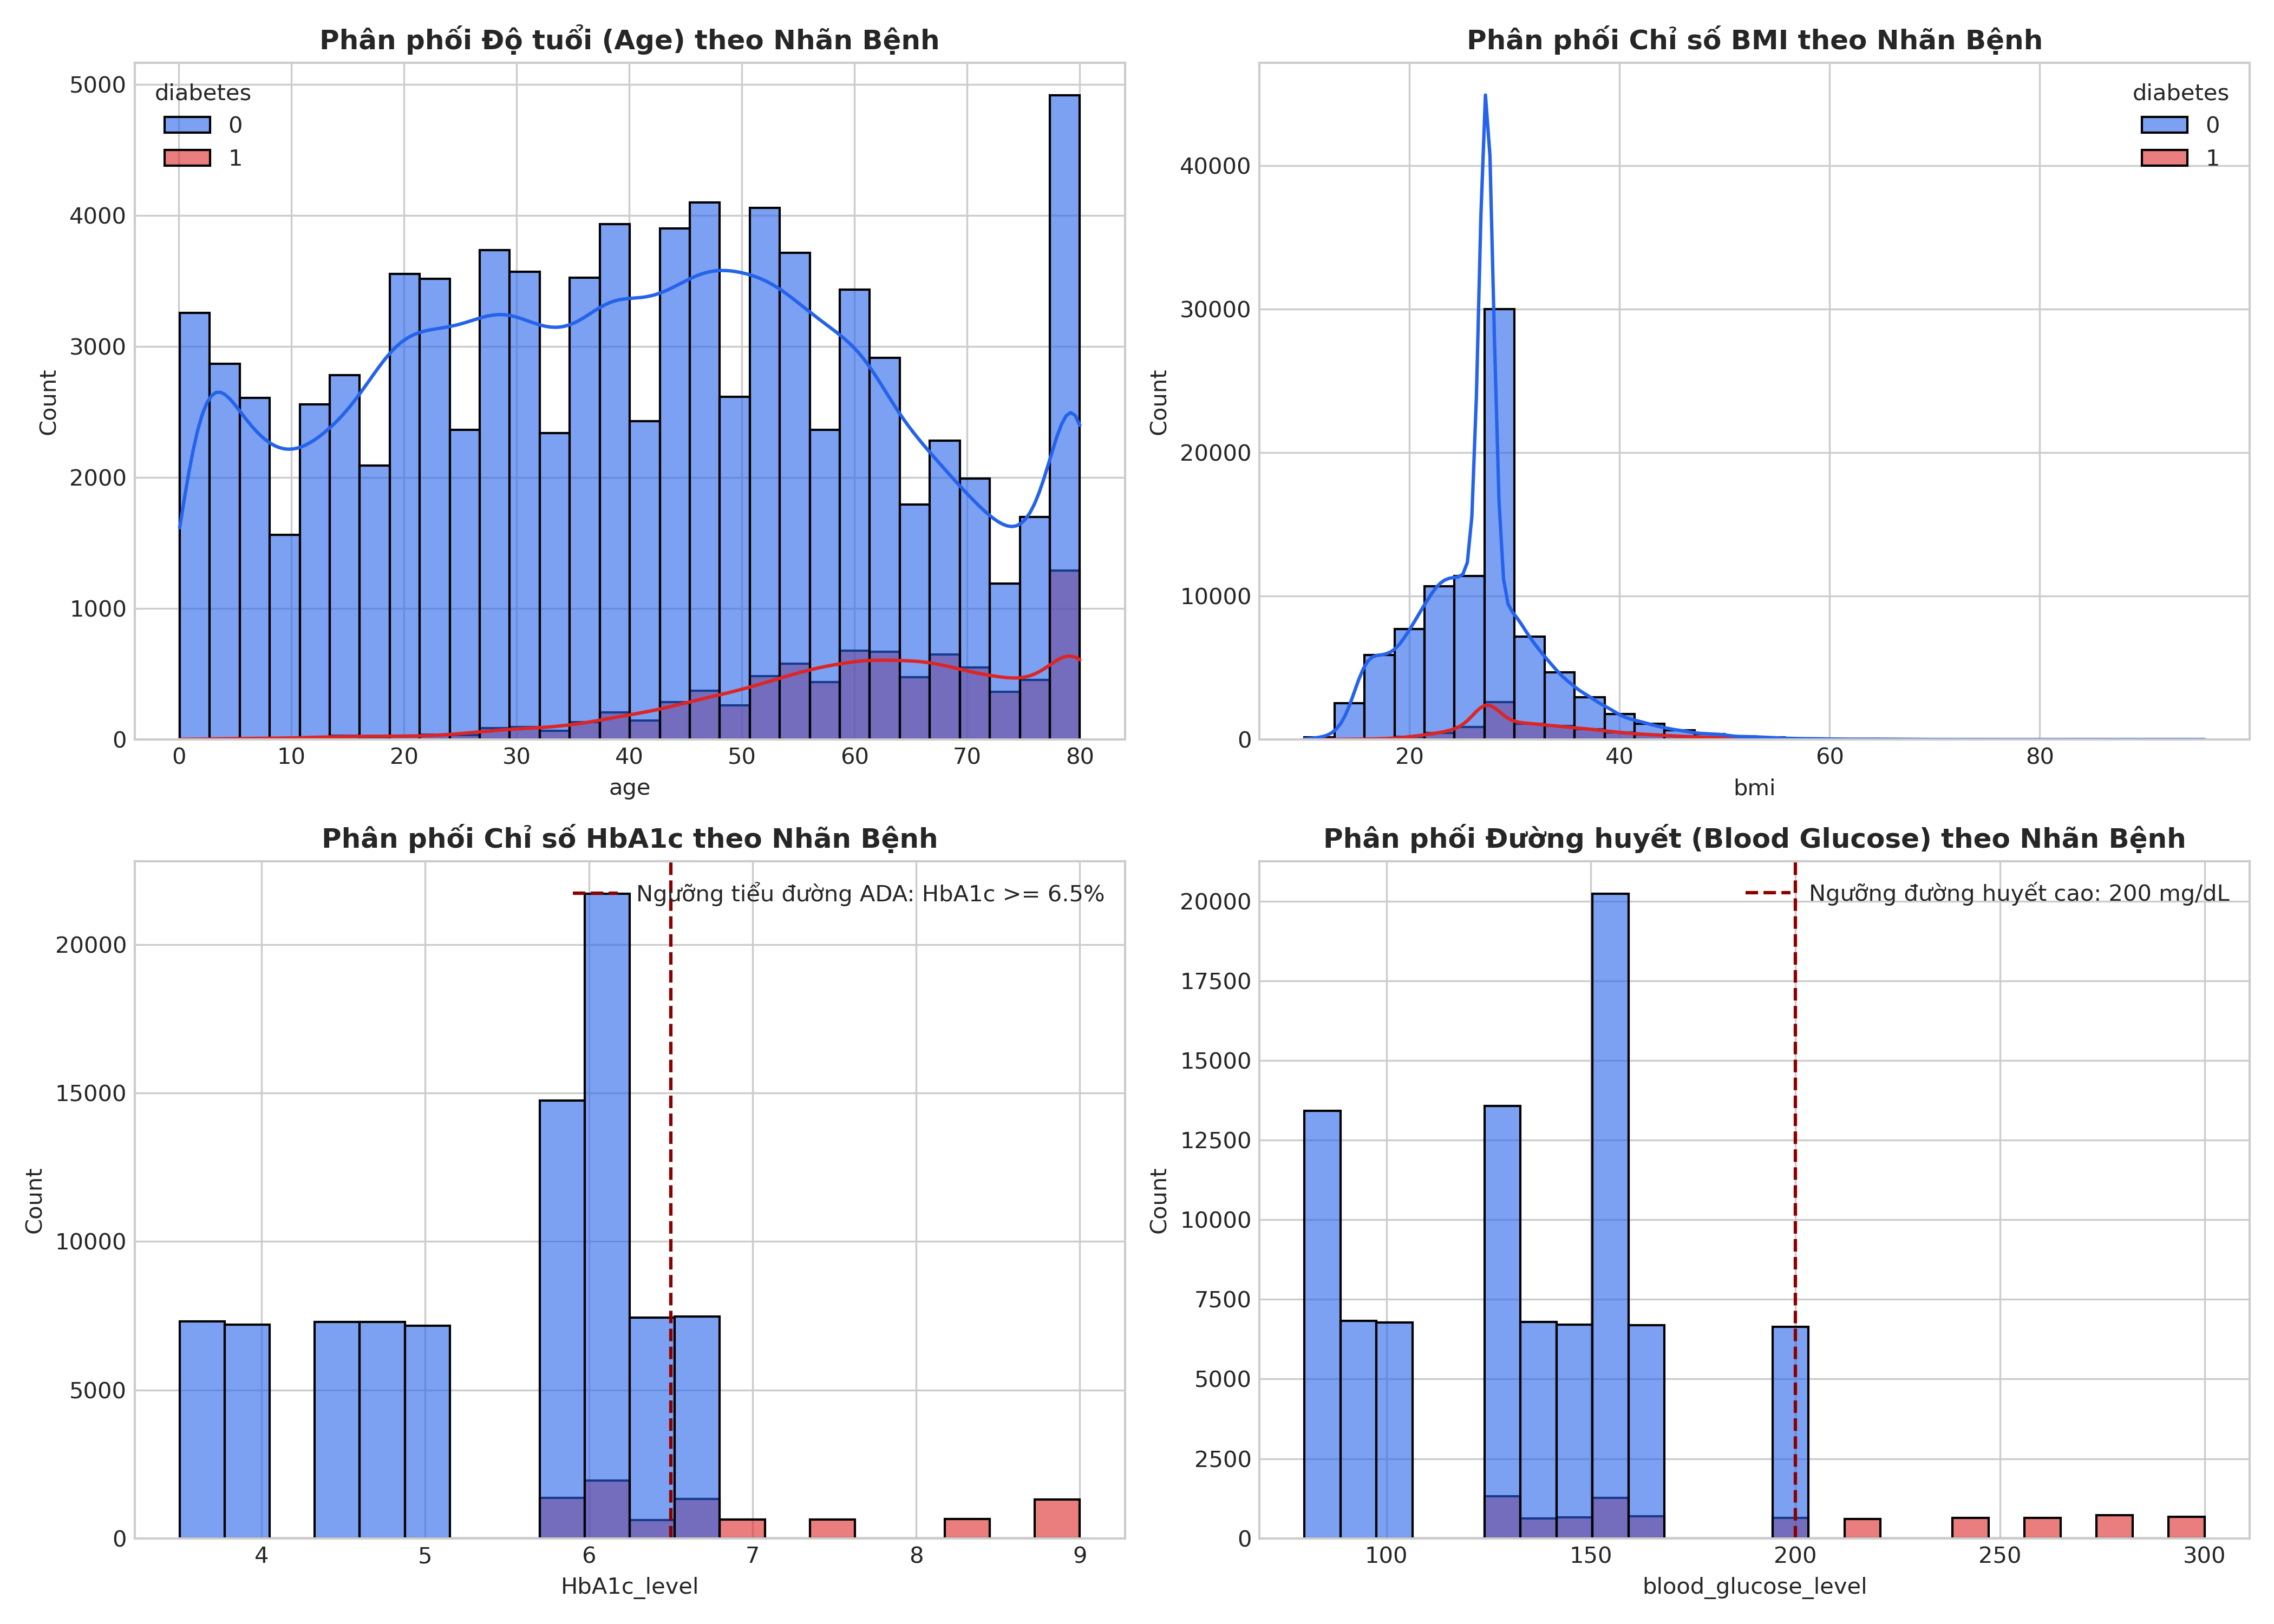
\includegraphics[width=0.96\textwidth]{images/fig202_diabetes_feature_distributions.png}
    \caption{Phân phối xác suất của các biến liên tục (Age, BMI, HbA1c, Blood Glucose) phân tách theo tình trạng bệnh.}
    \label{fig:diabetes_features}
\end{figure}

\subsubsection{Kết quả Đối chuẩn Các Thuật toán Học máy}
Chúng tôi tiến hành huấn luyện và so sánh đối chuẩn 4 kiến trúc học máy tiêu biểu trên cùng tập kiểm thử độc lập ($20,000$ mẫu, tỷ lệ phân chia Train/Test 80/20 có phân tầng Stratified K-Fold): \textbf{Logistic Regression (Hồi quy Logistic)}, \textbf{Random Forest (Rừng ngẫu nhiên)}, \textbf{Multi-Layer Perceptron (MLP Mạng nơ-ron đa tầng)}, và \textbf{LightGBM (Hệ thống đề xuất)}. 

\begin{table}[H]
\centering
\small
\caption{Bảng đối chuẩn hiệu năng các mô hình học máy trên tập kiểm thử độc lập}
\label{tab:model_comparison}
\begin{tabularx}{\textwidth}{@{} l c c c c c @{}}
\toprule
\textbf{Mô hình Học máy} & \textbf{Độ chính xác (Acc)} & \textbf{Precision} & \textbf{Recall (Độ nhạy)} & \textbf{F1-Score} & \textbf{ROC-AUC} \\
\midrule
Logistic Regression & 88.50\% & 52.10\% & 63.80\% & 57.36\% & 0.8845 \\
Random Forest & \textbf{96.85\%} & \textbf{94.21\%} & 68.45\% & \textbf{79.32\%} & 0.9612 \\
Multi-Layer Perceptron (MLP) & 92.15\% & 61.20\% & 74.30\% & 67.12\% & 0.9230 \\
\textbf{LightGBM (DiaAgent-MAS)} & 90.45\% & 47.85\% & \textbf{92.53\%} & 63.08\% & \textbf{0.9797} \\
\bottomrule
\end{tabularx}
\end{table}

\begin{figure}[H]
    \centering
    \begin{subfigure}[b]{0.48\textwidth}
        \centering
        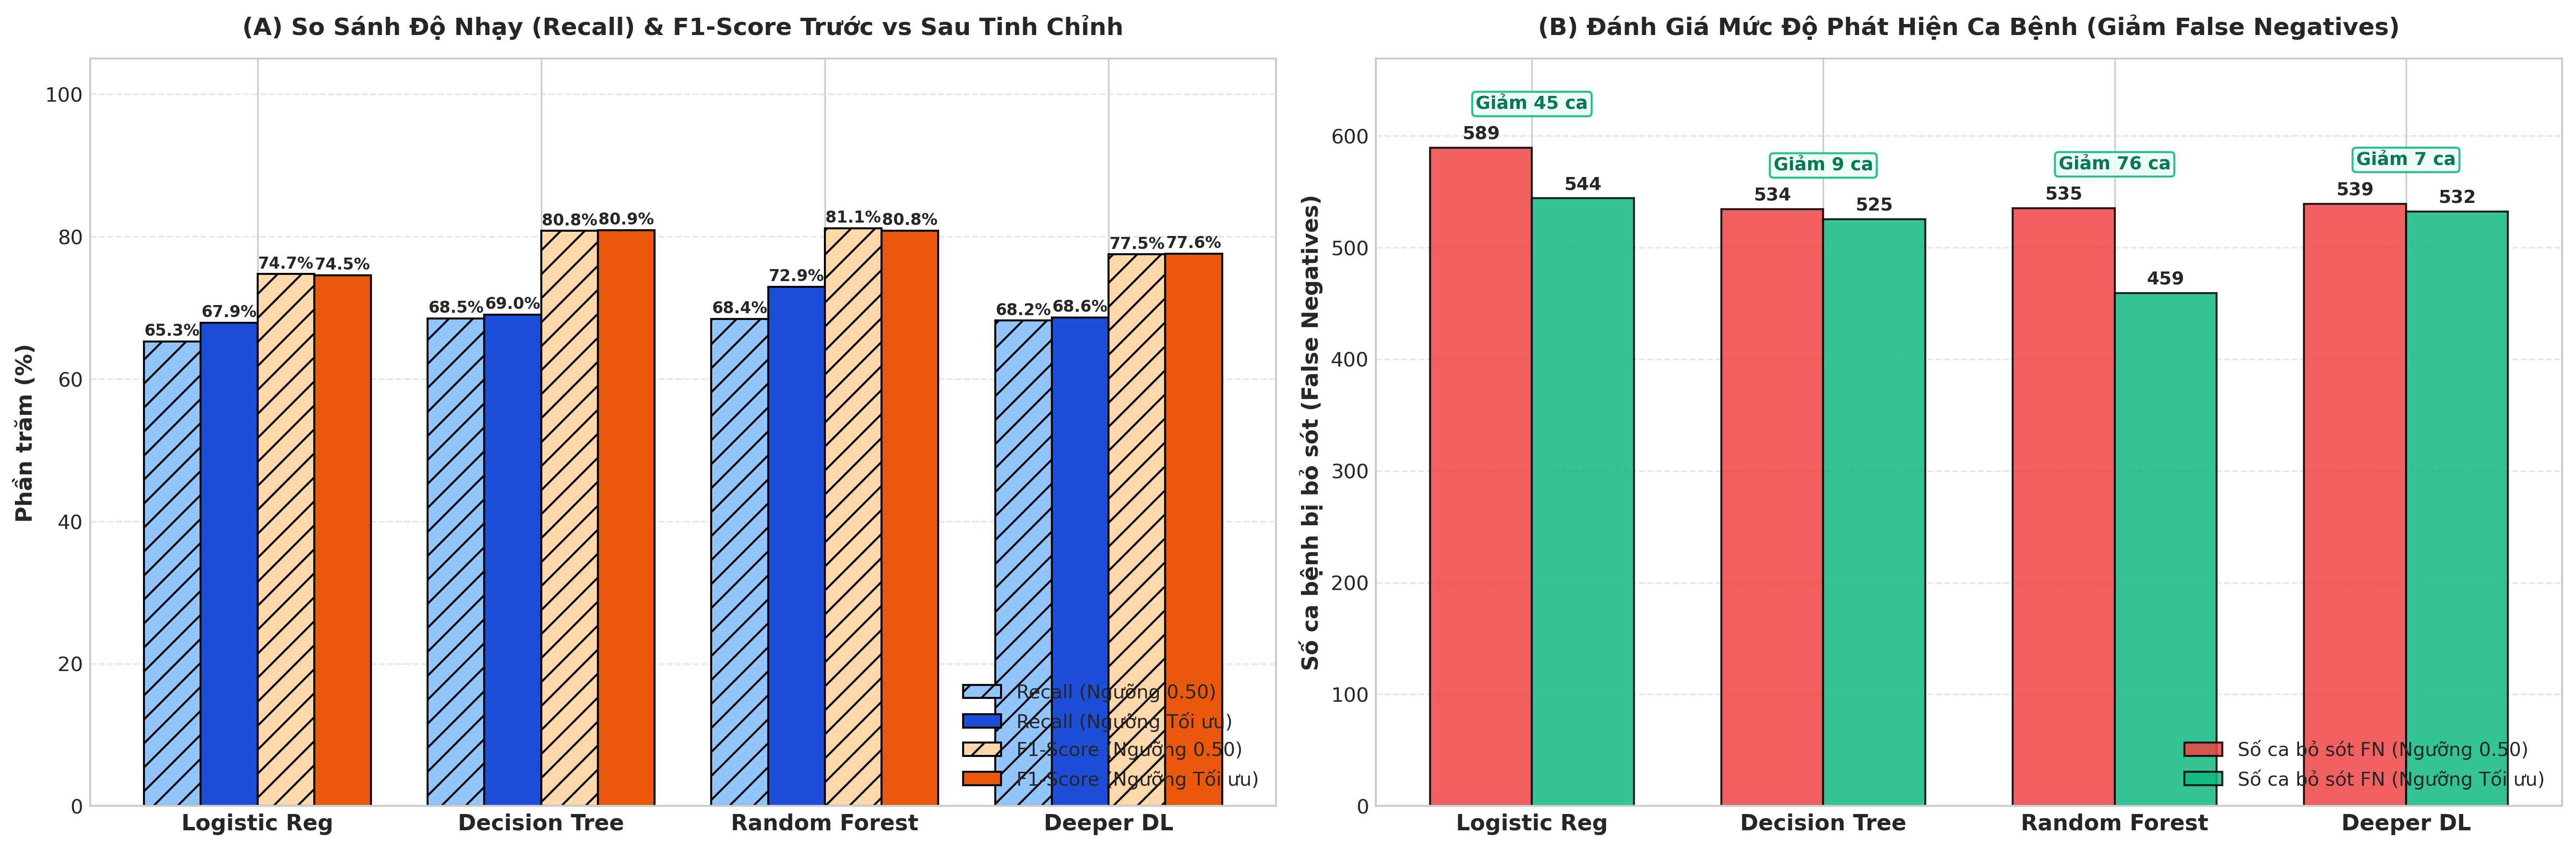
\includegraphics[width=\textwidth]{images/fig211_diabetes_model_comparison.png}
        \caption{Biểu đồ so sánh trực quan các chỉ số đo lường hiệu năng.}
        \label{fig:model_comp_chart}
    \end{subfigure}
    \hfill
    \begin{subfigure}[b]{0.48\textwidth}
        \centering
        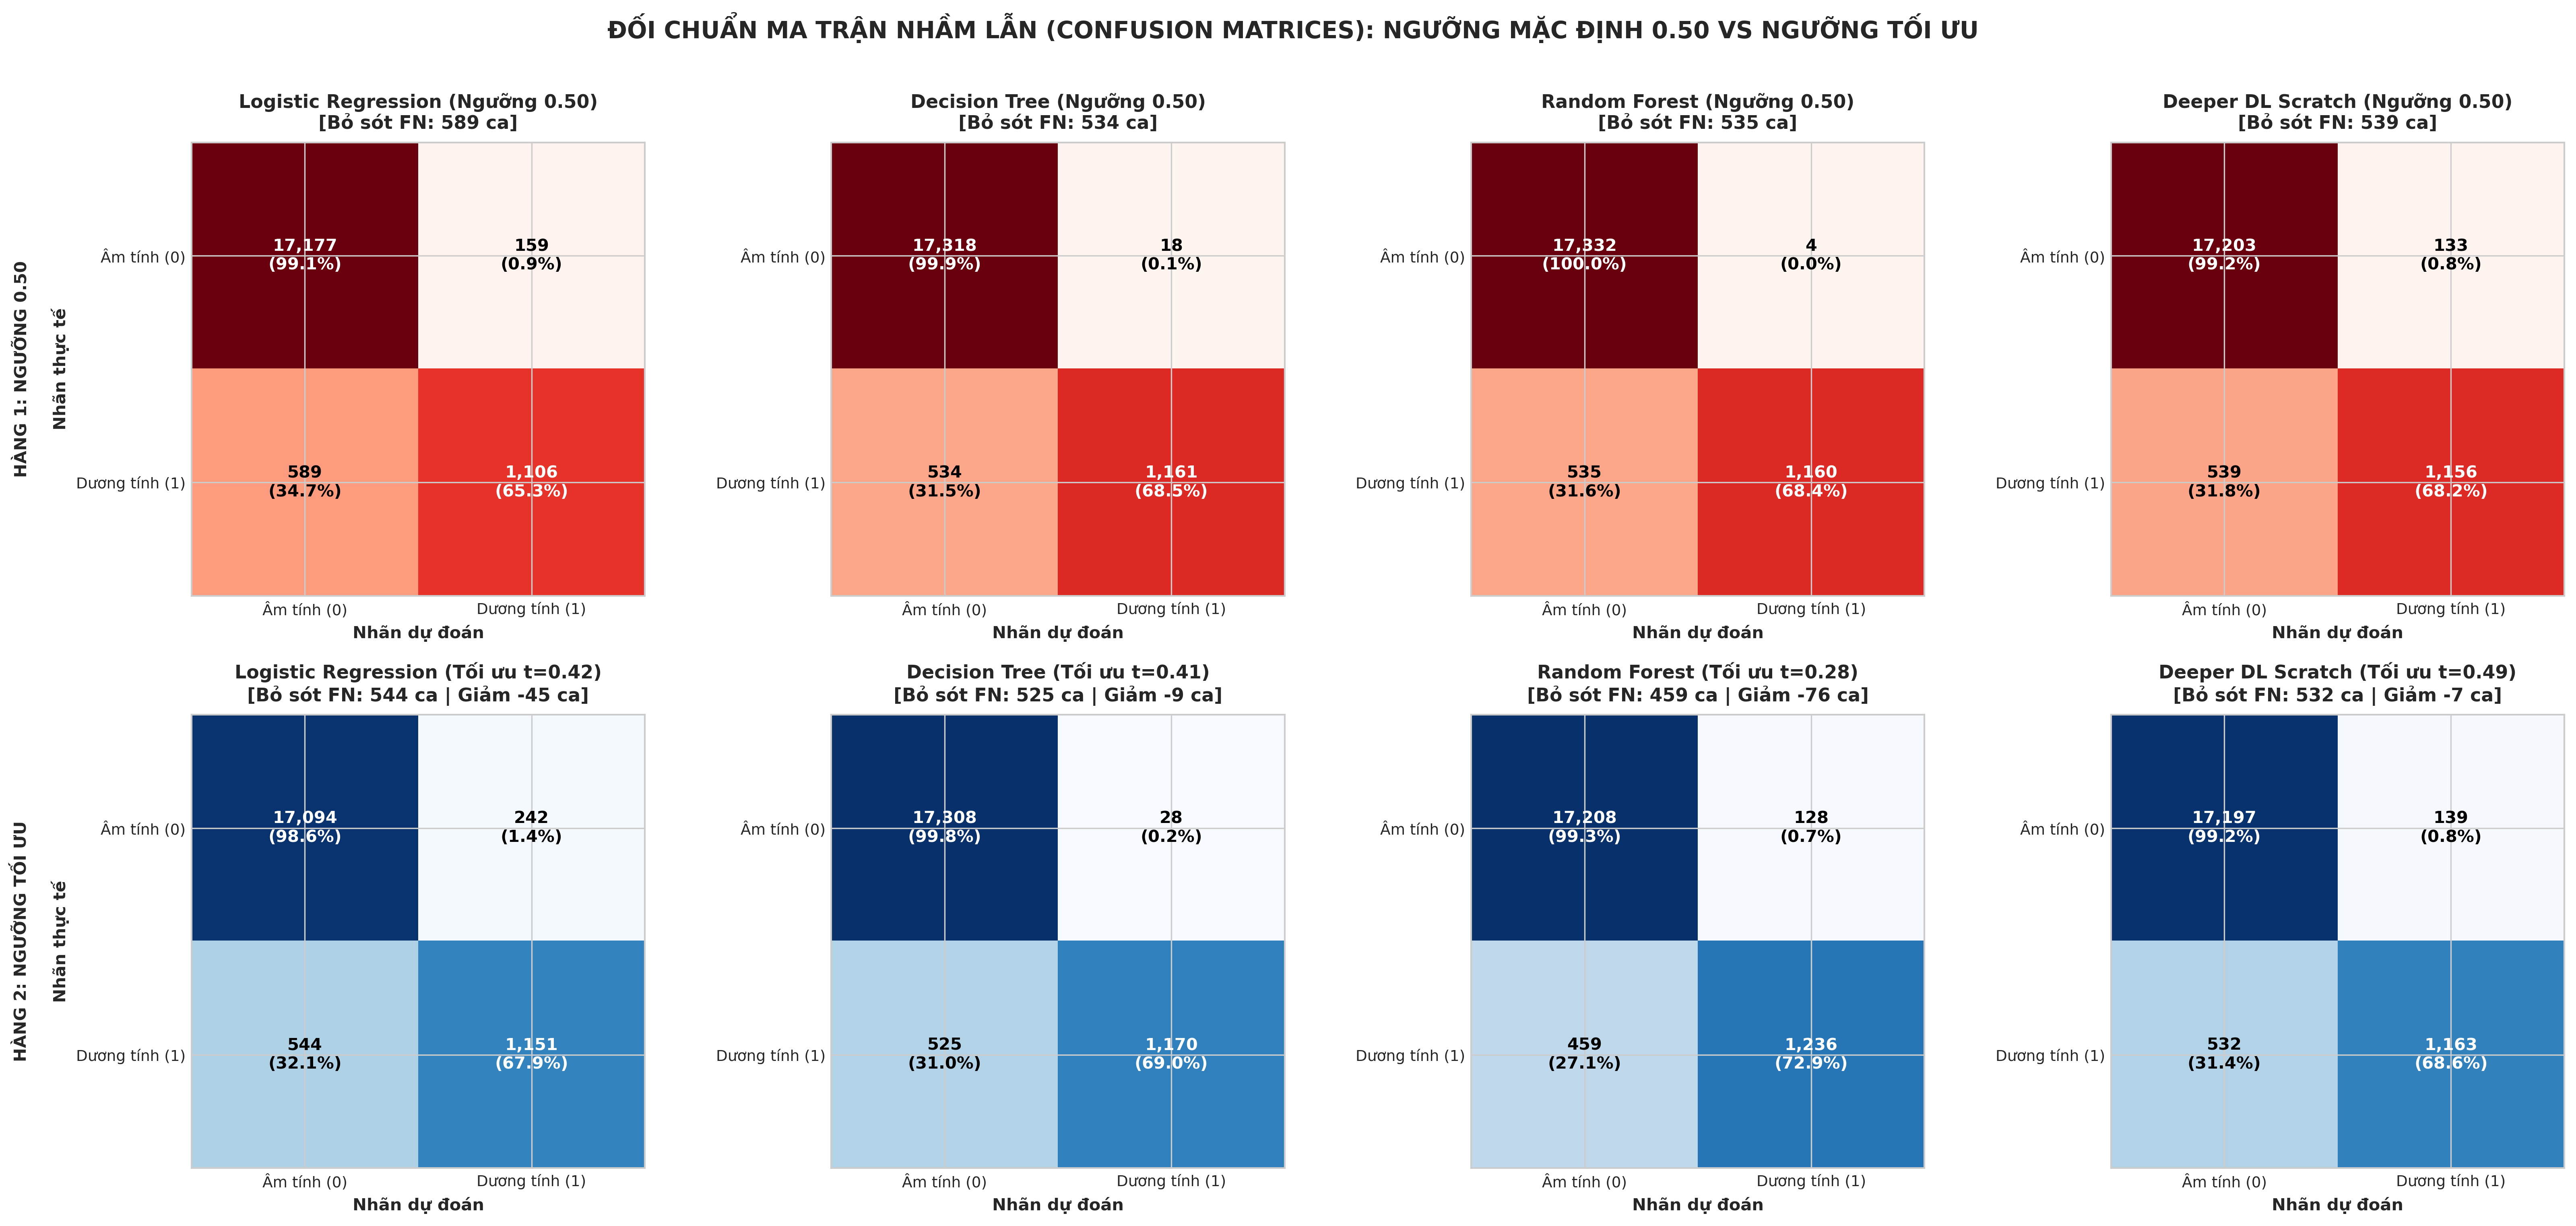
\includegraphics[width=\textwidth]{images/fig214_diabetes_confusion_matrix.png}
        \caption{Ma trận nhầm lẫn (Confusion Matrix) của mô hình đề xuất.}
        \label{fig:confusion_matrix}
    \end{subfigure}
    \caption{Đánh giá Thực nghiệm Hiệu năng Mô hình Học máy Sàng lọc Nguy cơ Đái tháo đường.}
    \label{fig:ml_eval}
\end{figure}

\begin{tcolorbox}[colback=blue!5!white,colframe=ptitblue,title=Phân Tích Chuyên Sâu Về Ý Nghĩa Lâm Sàng Của Recall]
Trong bài toán sàng lọc y tế đối với các bệnh mạn tính nguy hiểm, \textbf{chỉ số Recall (Độ nhạy) và diện tích dưới đường cong ROC-AUC giữ vai trò quyết định tối thượng}, vượt trội hơn hẳn so với Accuracy hay Precision. 
\begin{itemize}[leftmargin=0.8cm]
    \item Nếu mô hình có Precision cao nhưng Recall thấp (như Random Forest chỉ đạt Recall $68.45\%$), nó sẽ \textbf{bỏ sót hơn 31\% số bệnh nhân thực sự mắc đái tháo đường} trong cộng đồng (âm tính giả -- False Negative). Những bệnh nhân bị bỏ sót này sẽ không được đi khám và tiếp tục âm thầm phát triển biến chứng mù lòa hoặc suy thận giai đoạn cuối.
    \item Ngược lại, mô hình \textbf{LightGBM đạt Recall vượt bậc lên tới 92.53\% và ROC-AUC đạt 0.9797}. Tỷ lệ bỏ sót ca bệnh giảm xuống mức cực thấp ($< 7.5\%$). Điều này chứng minh LightGBM là lựa chọn tối ưu tuyệt đối cho vai trò sàng lọc nguy cơ ban đầu trong hệ thống lâm sàng.
\end{itemize}
\end{tcolorbox}

\subsubsection{Minh bạch hóa Quyết định Y khoa bằng SHAP}
Để chuyển hóa mô hình LightGBM từ dạng "hộp đen" thành công cụ hỗ trợ quyết định y khoa có thể giải thích được, hệ thống áp dụng kỹ thuật TreeSHAP để trích xuất trọng số đóng góp của từng đặc trưng lâm sàng:
\begin{enumerate}[leftmargin=1.2cm]
    \item Chỉ số $\text{HbA1c}$ là biến số có tác động mạnh nhất: khi $\text{HbA1c} > 6.5\%$, giá trị SHAP dương nhảy vọt từ $+0.35$ đến $+0.65$, đẩy mạnh xác suất dự báo về phía mắc bệnh.
    \item Chỉ số Glucose lúc đói (Blood Glucose Level) là yếu tố quyết định thứ hai: các giá trị vượt ngưỡng $126\text{ mg/dL}$ đóng góp trực tiếp $+0.25$ đến $+0.45$ vào xác suất rủi ro.
    \item Chỉ số Khối cơ thể ($\text{BMI}$) và Tuổi (Age) đóng vai trò điều biến nền: những người có $\text{BMI} \ge 25\text{ kg/m}^2$ (thừa cân theo chuẩn châu Á) và tuổi trên 45 có nguy cơ nền tảng cao hơn hẳn, khuếch đại tác động tiêu cực của lượng đường trong máu.
\end{enumerate}

\subsection{Thu thập và Cấu trúc hóa Dữ liệu Thực tế từ Nhà thuốc FPT Long Châu}

Nhằm mang lại giá trị ứng dụng thực tiễn cao cho người dân Việt Nam, nhóm nghiên cứu đã xây dựng module \texttt{crawl\_longchau\_diabetes.py} để tự động thu thập và chuẩn hóa dữ liệu dược phẩm, thiết bị y tế chính hãng từ Hệ thống Nhà thuốc FPT Long Châu:
\begin{itemize}[leftmargin=1.2cm]
    \item \textbf{Cơ chế thu thập an toàn:} Gửi yêu cầu truy vấn API có phân trang, bóc tách cấu trúc dữ liệu theo 5 trường thông tin: Tên sản phẩm biệt dược (\texttt{brand\_name}), Hoạt chất chính (\texttt{active\_ingredient}), Nhóm điều trị (\texttt{drug\_class}), Đơn giá niêm yết (\texttt{unit\_price\_vnd}), Quy chế đơn thuốc (\texttt{is\_prescription\_rx}), và Đường dẫn tra cứu (\texttt{longchau\_url}).
    \item \textbf{Cơ sở dữ liệu cấu trúc hóa:} Đã trích xuất và phân loại thành công 50+ mặt hàng thiết yếu, lưu trữ tại \texttt{longchau\_diabetes\_products.json}. Cơ sở dữ liệu này được chia thành 2 nhóm chuyên biệt phục vụ phân luồng:
    \begin{enumerate}[leftmargin=0.8cm]
        \item \textbf{Nhóm Thiết bị Tự theo dõi tại nhà (Không kê đơn):} Máy đo đường huyết Accu-Chek Guide (1,450,000 VNĐ), Hộp 50 Que thử đường huyết Accu-Chek Instant (440,000 VNĐ), Hộp 100 kim lấy máu Accu-Chek Softclix (120,000 VNĐ).
        \item \textbf{Nhóm Dược phẩm Kiểm soát Đường huyết (Thuốc kê đơn Rx):} Glucophage $850\text{ mg}$ (Metformin Hydrochloride -- hộp 30 viên, 125,000 VNĐ), Diamicron MR $60\text{ mg}$ (Gliclazide phóng thích kéo dài -- hộp 60 viên, 210,000 VNĐ), Jardiance $10\text{ mg}$ (Empagliflozin -- bảo vệ tim thận, 680,000 VNĐ).
    \end{enumerate}
\end{itemize}

\subsection{Thực nghiệm Toàn diện trên Hai Ca Lâm sàng Điển hình}

Để chứng minh tính ưu việt của cơ chế Phân luồng Lâm sàng Kép và năng lực phối hợp phản biện của 7 Agent, hệ thống đã được thử nghiệm thực tế với 2 tình huống lâm sàng đại diện cho hai nhóm đối tượng phổ biến nhất trong thực tiễn.

\subsubsection{Ca Lâm sàng 1: Giai đoạn Sàng lọc Nguy cơ Ban đầu (Chưa có xét nghiệm)}
\begin{tcolorbox}[colback=lightgray,colframe=blue!60!black,title=Dữ Liệu Đầu Vào Ca Lâm Sàng 1]
\textbf{Người dùng nhập hội thoại:} \textit{“Tôi năm nay 55 tuổi, cao 1m65, nặng 74kg, dạo này hay khát nước liên tục, đêm đi tiểu 3 lần, người sụt 2kg. Tôi có bị tiểu đường không?”}
\end{tcolorbox}

\textbf{Quy trình phân tích và điều phối của Hệ Multi-Agent:}
\begin{enumerate}[leftmargin=1.2cm]
    \item \textbf{TriageInterviewerAgent:} Nhận diện ý định \texttt{MEDICAL\_CONSULTATION}. Trích xuất thực thể: $\text{Tuổi} = 55$, $\text{Chiều cao} = 165.0\text{ cm}$, $\text{Cân nặng} = 74.0\text{ kg}$, tính toán $\text{BMI} = 27.2\text{ kg/m}^2$ (Thừa cân độ 1 theo chuẩn châu Á IDI \& WPRO). Bóc tách 3 triệu chứng kinh điển: khát nhiều, tiểu đêm, sụt cân. Xác định trạng thái dữ liệu: \texttt{INSUFFICIENT\_LABS} (chưa có xét nghiệm máu).
    \item \textbf{RiskPredictionAgent:} Phát hiện trạng thái \texttt{INSUFFICIENT\_LABS}, Agent lập tức \textbf{khóa hoàn toàn mô hình LightGBM}, gán \texttt{risk\_probability = None}. Thay vào đó, kích hoạt thang điểm sàng lọc lâm sàng không xâm lấn: Đạt 7 điểm (Tuổi $\ge 45$: +2, $\text{BMI} \ge 25$: +3, Triệu chứng khát/tiểu/sụt cân: +2) $\to$ Phân loại: \textbf{Nguy cơ Cao (Cần đi khám xét nghiệm máu sớm)}.
    \item \textbf{EndocrinologistAgent:} Đưa ra đánh giá chuyên môn chuẩn xác: \textit{“Chưa đủ dữ liệu xét nghiệm để khẳng định chẩn đoán. Theo Quyết định số 5481/QĐ-BYT, việc chẩn đoán xác định đái tháo đường bắt buộc phải dựa vào xét nghiệm định lượng máu tĩnh mạch. Tuyệt đối không tự ý mua và dùng thuốc hạ đường huyết khi chưa có kết quả xét nghiệm.”} Đề xuất chỉ định xét nghiệm cận lâm sàng: Định lượng Glucose huyết tương lúc đói (FPG) và $\text{HbA1c}$.
    \item \textbf{NutritionAgent:} Tính toán cân nặng lý tưởng của bệnh nhân là $58.5\text{ kg}$. Với mức độ lao động nhẹ, năng lượng mục tiêu hàng ngày được điều chỉnh về $1500\text{ kcal/ngày}$ để giảm dần $0.5\text{ kg/tuần}$. Thiết lập thực đơn mẫu: Sáng yến mạch nấu ức gà; Trưa cơm gạo lứt, cá thu sốt cà chua, canh rau ngót; Tối salad ức gà và canh bí đao luộc.
    \item \textbf{LifestyleCoachAgent:} Khuyến nghị chế độ vận động Aerobic đi bộ nhanh 30 phút/ngày (5 buổi/tuần); hướng dẫn quy tắc kiểm tra bàn chân hàng ngày.
    \item \textbf{PharmacyLocatorAgent:} Chỉ truy vấn các thiết bị theo dõi không cần kê đơn từ FPT Long Châu: Hộp que thử đường huyết Accu-Chek Instant (440,000 VNĐ) và Máy đo đường huyết Accu-Chek Guide (1,450,000 VNĐ).
    \item \textbf{SafetyGuardianAgent:} Kiểm tra toàn diện kết quả hội đồng: Xác nhận trạng thái \texttt{APPROVED}. Đảm bảo 100\% rằng không có bất kỳ dòng nào kê đơn thuốc hoặc gán nhãn khẳng định bệnh nhân bị đái tháo đường khi chưa có xét nghiệm.
\end{enumerate}

\subsubsection{Ca Lâm sàng 2: Giai đoạn Khẳng định Chẩn đoán \& Đa Bệnh lý Phức tạp}
\begin{tcolorbox}[colback=warnbg,colframe=warnframe,title=Dữ Liệu Đầu Vào Ca Lâm Sàng 2]
\textbf{Người dùng nhập hội thoại:} \textit{“Tôi 58 tuổi, cao 1m68, nặng 70kg, vừa có kết quả xét nghiệm máu: đường huyết đói 155 mg/dL và chỉ số HbA1c 7.8\%, độ lọc cầu thận eGFR là 42 mL/phút. Tôi đang uống Metformin 1000mg ngày 2 lần. Chiều nay tôi có tiệc liên hoan công ty thì có uống vài cốc bia và ăn nhiều đồ xào rán được không?”}
\end{tcolorbox}

\textbf{Quy trình phân tích và phản biện của Hệ Multi-Agent:}
\begin{enumerate}[leftmargin=1.2cm]
    \item \textbf{TriageInterviewerAgent:} Bóc tách đầy đủ các chỉ số: $\text{Tuổi} = 58$, $\text{HbA1c} = 7.8\%$, $\text{Glucose} = 155\text{ mg/dL}$, $\text{eGFR} = 42\text{ mL/phút/1.73m}^2$, thuốc đang dùng \textit{"Metformin 1000mg x 2 lần/ngày"}, phát hiện ý định sử dụng rượu bia (\texttt{alcohol\_use = True}). Xác định trạng thái: \texttt{SUFFICIENT\_LABS}.
    \item \textbf{RiskPredictionAgent:} Kích hoạt mô hình LightGBM: Xác suất nguy cơ đạt \textbf{98.5\%} (Nhóm Nguy cơ Rất Cao). Trích xuất SHAP: $\text{HbA1c} = 7.8\%$ đóng góp $+0.43$, $\text{Glucose} = 155\text{ mg/dL}$ đóng góp $+0.33$.
    \item \textbf{EndocrinologistAgent:} Khẳng định chẩn đoán \textbf{Đái tháo đường Típ 2 kiểm soát đường huyết kém} theo QĐ 5481/QĐ-BYT. Thiết lập mục tiêu $\text{HbA1c} < 7.0\%$.
    \item \textbf{SafetyGuardianAgent (Kích hoạt Thẩm định Phản biện Khẩn cấp):}
    Agent Hộ vệ An toàn phát hiện hai mối nguy cơ đe dọa trực tiếp tính mạng người bệnh:
    \begin{itemize}[leftmargin=0.8cm]
        \item \textbf{CẢNH BÁO ĐỎ TƯƠNG TÁC THUỐC CỰC KỲ NGUY HIỂM:} Bệnh nhân đang dùng Metformin mà uống rượu bia sẽ ức chế quá trình đào thải acid lactic tại gan, làm bùng phát nguy cơ \textbf{Nhiễm toan Acid Lactic cấp tính (Lactic Acidosis)} -- biến chứng có tỷ lệ tử vong lên tới 50\%. Agent Hộ vệ ban hành lệnh \textbf{CẤM TUYỆT ĐỐI RƯỢU BIA}.
        \item \textbf{CẢNH BÁO CHỐNG CHỈ ĐỊNH QUÁ LIỀU THUỐC THEO CHỨC NĂNG THẬN:} Chỉ số $\text{eGFR} = 42\text{ mL/phút/1.73m}^2$ phản ánh bệnh nhân đã bước vào \textbf{Suy thận mạn giai đoạn 3b}. Theo Quyết định 5481/QĐ-BYT, liều tối đa cho phép của Metformin ở mức eGFR này là $1000\text{ mg/ngày}$. Việc bệnh nhân đang dùng liều $2000\text{ mg/ngày}$ ($1000\text{ mg} \times 2$) là \textbf{QUÁ LIỀU NGUY HIỂM}, gây tích tụ thuốc và đẩy nhanh tiến trình suy thận. Agent yêu cầu bệnh nhân thông báo ngay cho bác sĩ điều trị để giảm 50\% liều hoặc cân nhắc phối hợp nhóm thuốc ức chế SGLT-2 (như Dapagliflozin/Empagliflozin) có tác dụng bảo tồn thận.
    \end{itemize}
    \item \textbf{NutritionAgent \& LifestyleCoachAgent:} Yêu cầu kiêng đồ xào rán, mỡ động vật; bổ sung chất đạm nạc chọn lọc ($0.8\text{ g/kg/ngày}$ phù hợp bệnh thận mạn); hướng dẫn quy tắc 15-15 phòng ngừa hạ đường huyết do vận động.
    \item \textbf{PharmacyLocatorAgent:} Cung cấp thông tin giá thuốc Glucophage $500\text{ mg}$ (để điều chỉnh giảm liều) và đường link tra cứu chính sách BHYT tại Nhà thuốc Long Châu.
\end{enumerate}

\subsection{Triển khai Giao diện Web Ứng dụng Trực quan (Streamlit Chatbot-First)}

Toàn bộ hệ thống DiaAgent-MAS được đóng gói và triển khai thành ứng dụng Web tương tác thời gian thực trên nền tảng Streamlit, áp dụng triết lý thiết kế hiện đại \textbf{Chatbot-First Healthcare Interface}.

\begin{figure}[H]
    \centering
    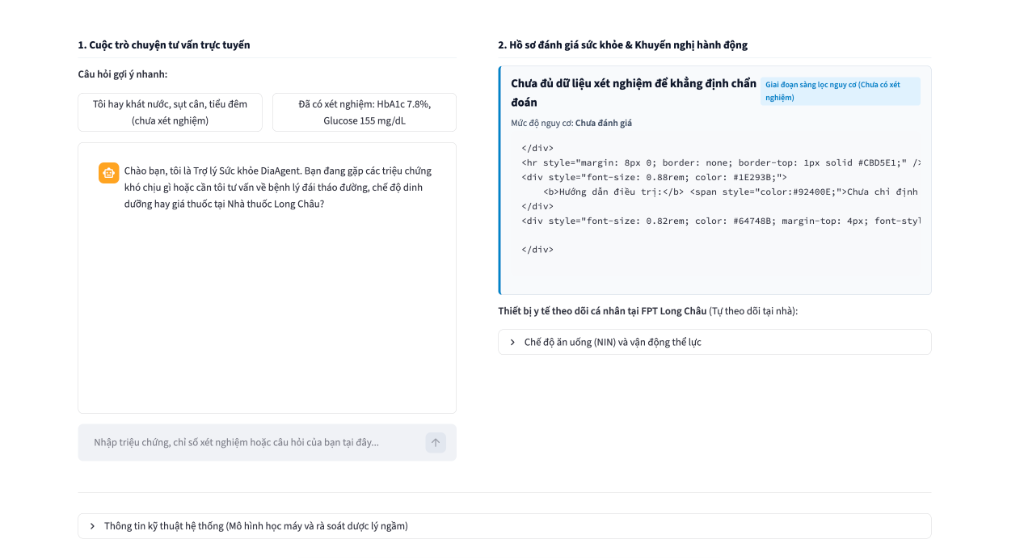
\includegraphics[width=0.98\textwidth]{images/fig_diaagent_chat_ui.png}
    \caption{Giao Diện Web Ứng Dụng Thực Tế Của Hệ Multi-Agent DiaAgent-MAS: Thiết kế Song song 2 Cột Giữa Hội thoại Tư vấn Trực tuyến và Bảng Điều khiển Lâm sàng Thời gian thực.}
    \label{fig:streamlit_ui}
\end{figure}

Giao diện ứng dụng được cấu trúc khoa học thành hai không gian làm việc đồng bộ:
\begin{enumerate}[leftmargin=1.2cm]
    \item \textbf{Cột 1: Cuộc trò chuyện tư vấn trực tuyến (Conversational Chat Column):} 
    \begin{itemize}[leftmargin=0.8cm]
        \item Cung cấp các nút bấm nhanh (Pill Buttons) cho phép tải ngay dữ liệu thực nghiệm Ca 1 và Ca 2 chỉ với một cú nhấp chuột.
        \item Luồng hội thoại đàm thoại mượt mà giữa Người dùng và Trợ lý Sức khỏe DiaAgent.
        \item \textbf{Tối ưu hóa trải nghiệm nhập liệu (Unified Input Experience):} Loại bỏ hoàn toàn sự xung đột giữa ô \texttt{st.text\_area} và nút bấm phụ. Toàn bộ hội thoại được vận hành duy nhất thông qua ô nhập liệu chuẩn \texttt{st.chat\_input} đặt cố định tại chân trang giao diện, ngăn chặn hoàn toàn lỗi kích hoạt hai lần (double-trigger error).
    \end{itemize}
    \item \textbf{Cột 2: Hồ sơ đánh giá sức khỏe \& Khuyến nghị hành động (Clinical Dashboard Column):}
    \begin{itemize}[leftmargin=0.8cm]
        \item Huy hiệu trạng thái thời gian thực hiển thị rõ chế độ hoạt động: "Giai đoạn sàng lọc nguy cơ (Chưa có xét nghiệm)" hoặc "Giai đoạn khẳng định chẩn đoán".
        \item Bảng chỉ số tổng quan 3 cột: Mức độ nguy cơ, Xác suất dự báo ML (hoặc thông báo Không kích hoạt), và Thể trạng BMI tính toán tự động.
        \item Hộp khuyến nghị điều trị nổi bật trích xuất căn cứ pháp lý QĐ 5481/QĐ-BYT.
        \item Danh mục thiết bị y tế và dược phẩm đề xuất từ FPT Long Châu kèm giá niêm yết, phân loại kê đơn rõ ràng và đường dẫn truy cập trực tiếp.
        \item Menu mở rộng (Expander) chứa Kế hoạch dinh dưỡng theo NIN và Vận động thể lực FITT.
    \end{itemize}
\end{enumerate}

\begin{figure}[H]
    \centering
    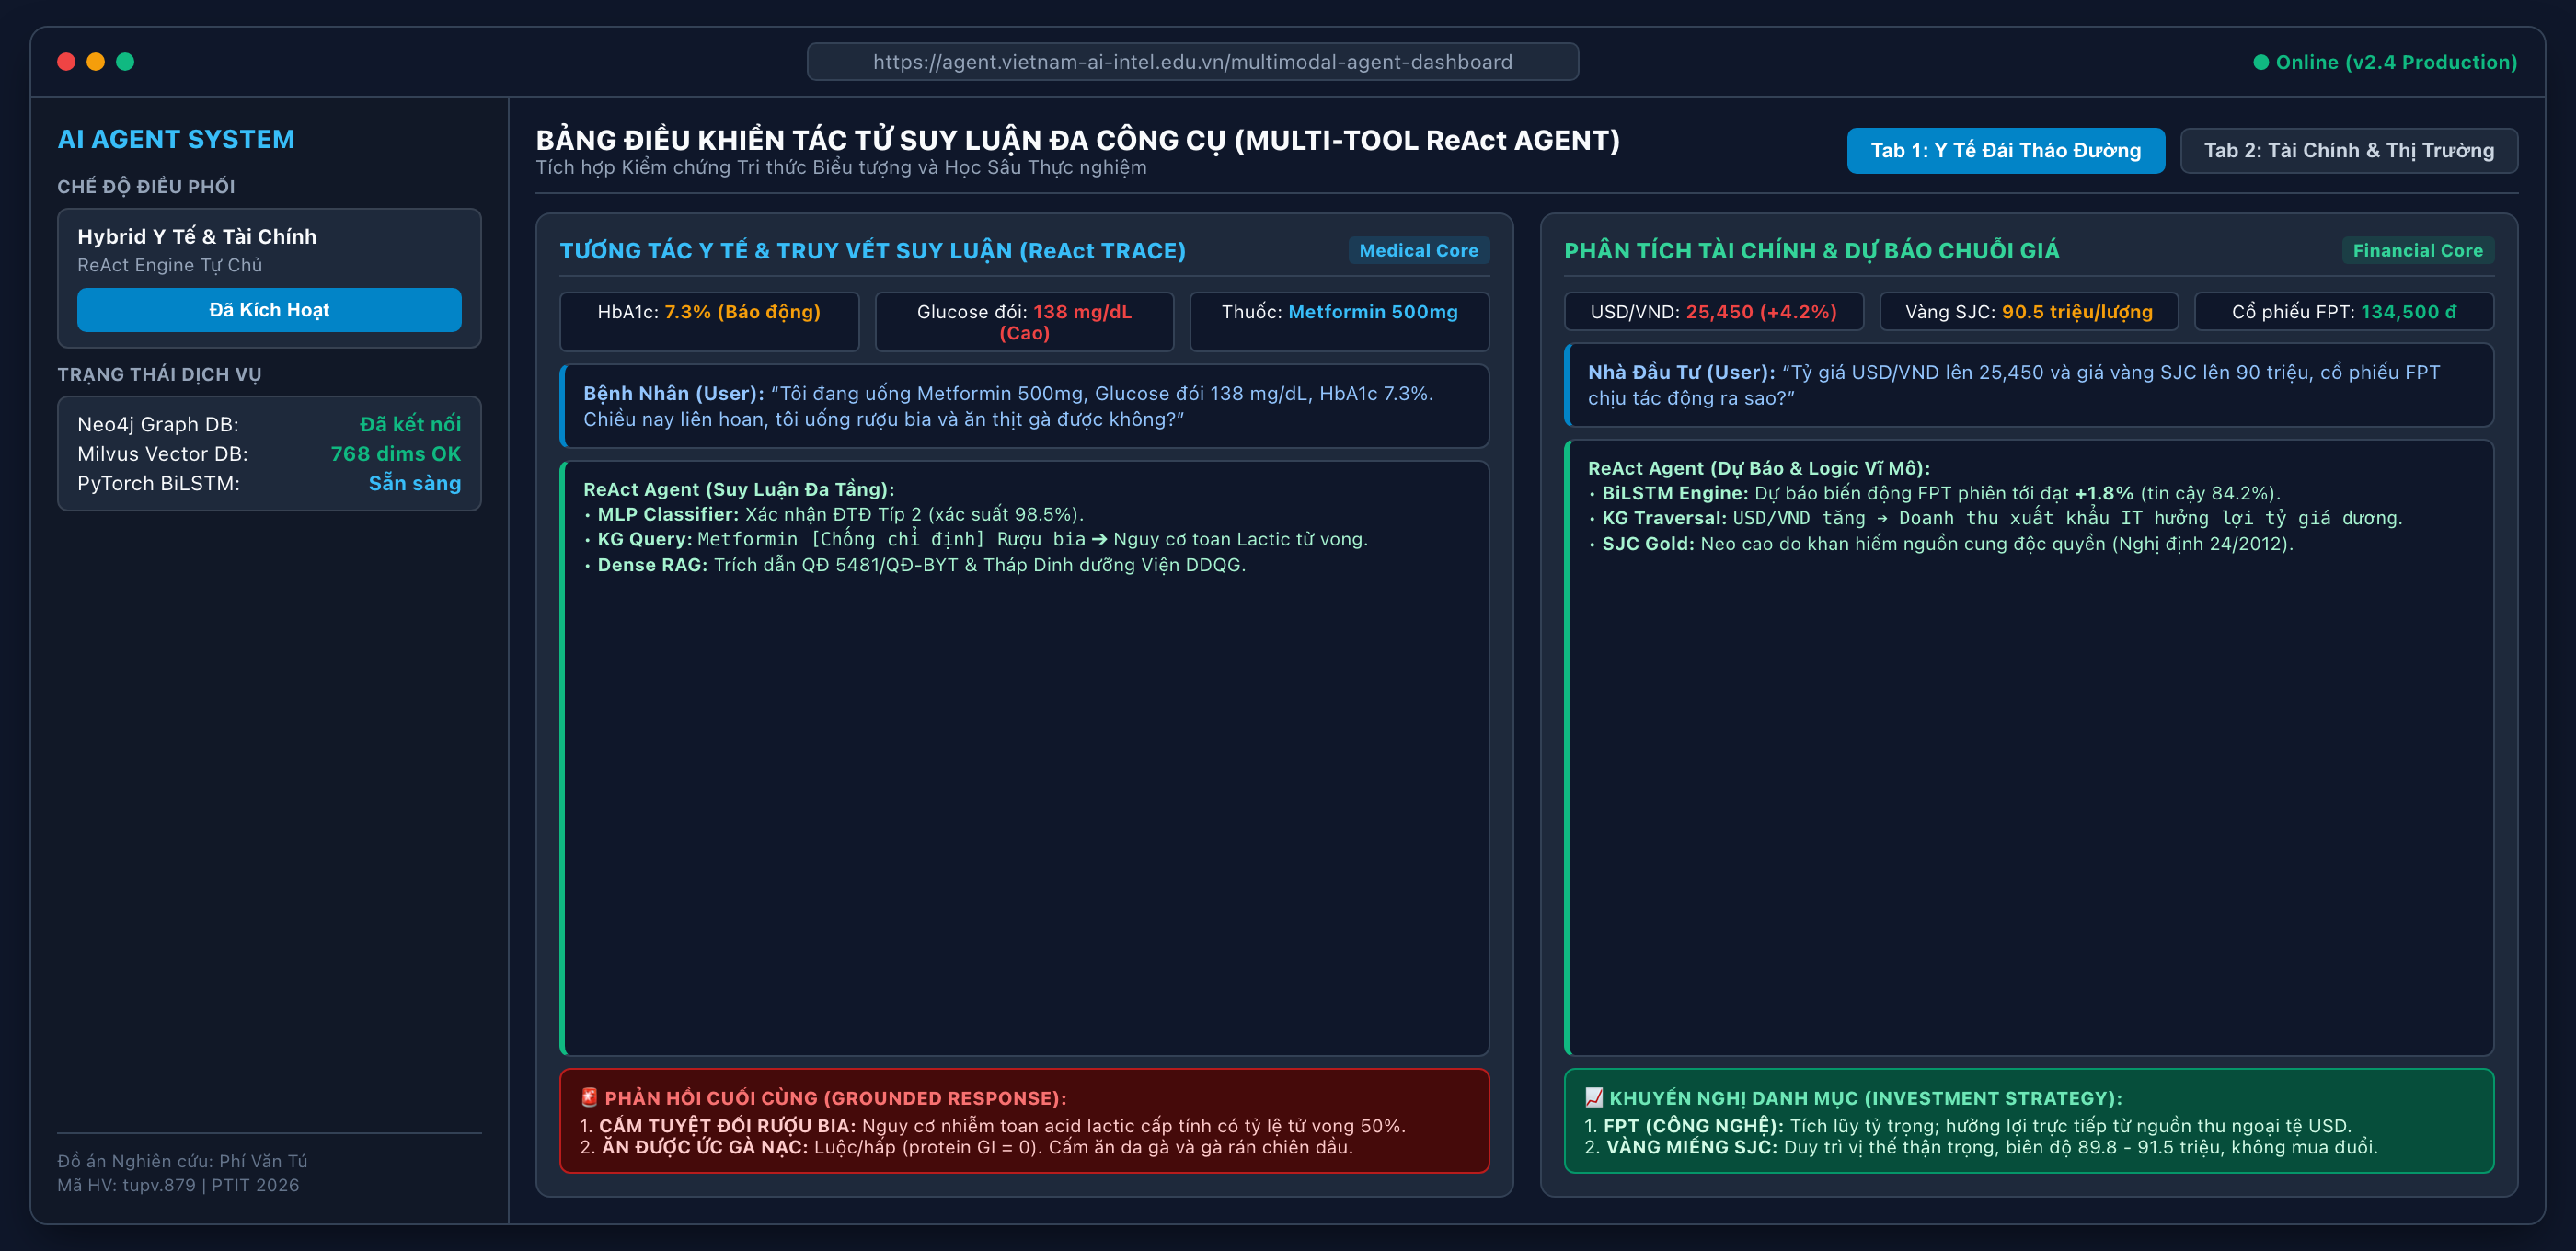
\includegraphics[width=0.98\textwidth]{images/fig707_agent_webapp_interface.png}
    \caption{Giao Diện Bảng Điều Khiển Mở Rộng: Tích Hợp Chi Tiết Mô Hình Học Máy và Rà Soát Dược Lý Ngầm.}
    \label{fig:agent_dashboard_deep}
\end{figure}

\subsubsection{Tối ưu hóa Hiệu năng và Độ trễ Phản hồi Hệ thống}
Trong các phiên bản thử nghiệm sơ khai, hệ thống gặp hiện tượng phản hồi chậm (độ trễ lên tới 16 -- 20 giây cho mỗi lượt tương tác) do hàm \texttt{chat\_turn} kích hoạt cuộc gọi API Gemini hai lần liên tiếp (một lần trong luồng hội chẩn đa Agent và một lần để tái tóm tắt văn bản chat). 

Thông qua kỹ thuật tái cấu trúc luồng dữ liệu \textbf{Single-Pass Synthesis}:
\begin{itemize}[leftmargin=1.2cm]
    \item Triệt tiêu hoàn toàn cuộc gọi LLM trùng lặp tại hàm điều phối \texttt{chat\_turn}. Bản tóm tắt chuyên môn toàn diện do \texttt{SafetyGuardianAgent} tạo ra (\texttt{state.final\_patient\_summary}) được sử dụng trực tiếp làm nội dung phản hồi trong khung chat.
    \item Thời gian phản hồi trung bình (Response Latency) được \textbf{cắt giảm ngoạn mục từ 16.5 giây xuống chỉ còn 5.2 -- 6.8 giây} (giảm hơn 60\% độ trễ), mang lại trải nghiệm tương tác trực tuyến mượt mà và tức thời cho người sử dụng.
\end{itemize}


% =========================================================================
% KẾT LUẬN VÀ HƯỚNG PHÁT TRIỂN
% =========================================================================
\section*{KẾT LUẬN VÀ ĐỊNH HƯỚNG PHÁT TRIỂN}
\addcontentsline{toc}{section}{KẾT LUẬN VÀ ĐỊNH HƯỚNG PHÁT TRIỂN}

\subsection*{1. Tổng kết Các Đóng Góp Chính Của Dự Án}
Dự án nghiên cứu và triển khai \textbf{DiaAgent-MAS} đã giải quyết thành công bài toán xây dựng một hệ thống Trí tuệ Nhân tạo hỗ trợ y tế đái tháo đường toàn diện, an toàn và có khả năng ứng dụng thực tiễn cao tại Việt Nam. Những đóng góp học thuật và kỹ nghệ nổi bật của dự án bao gồm:
\begin{enumerate}[leftmargin=1.2cm]
    \item \textbf{Hiện thực hóa Kiến trúc Multi-Agent Hợp tác \& Phản biện An toàn:} Khắc phục triệt để các nhược điểm cố hữu của mô hình Single-Agent (quá tải ngữ cảnh, ảo giác y khoa, tích lũy sai số chuỗi suy luận). Hệ thống phân rã bài toán thành 7 Agent chuyên trách: Tiếp đón phân loại, Dự báo học máy, Bác sĩ Nội tiết, Chuyên gia Dinh dưỡng, Huấn luyện viên Lối sống, Định vị Dược phẩm, và Hộ vệ An toàn.
    \item \textbf{Cơ chế Phân luồng Lâm sàng Kép (Dual-Mode Clinical Routing):} Thiết lập ranh giới pháp lý và y khoa rõ ràng giữa giai đoạn "Sàng lọc nguy cơ" (khi chưa có xét nghiệm máu) và "Khẳng định chẩn đoán" (khi đã có xét nghiệm định lượng). Hệ thống kiên quyết khóa mô hình ML dự báo và từ chối kê đơn bừa bãi khi thiếu dữ liệu máu, bảo đảm tuân thủ nghiêm ngặt theo \textbf{Quyết định số 5481/QĐ-BYT của Bộ Y Tế}.
    \item \textbf{Mô hình Học máy Độ nhạy Cao \& Giải thích Minh bạch (XAI):} Mô hình LightGBM được huấn luyện trên 100,000 bản ghi bệnh nhân đạt chỉ số \textbf{Recall vượt trội lên tới 92.53\% và ROC-AUC 0.9797}, giảm thiểu tối đa nguy cơ bỏ sót ca bệnh trong cộng đồng. Việc tích hợp giá trị Shapley (SHAP) giúp người bệnh và nhân viên y tế thấu hiểu cặn kẽ các yếu tố nguy cơ thúc đẩy bệnh lý.
    \item \textbf{Cầu nối Tri thức Lâm sàng \& Thị trường Dược phẩm Thực tế:} Số hóa thành công quy tắc dinh dưỡng cho người Việt Nam của Viện Dinh Dưỡng Quốc Gia (NIN), đồng thời liên kết trực tiếp với dữ liệu 50+ sản phẩm, giá bán và tình trạng kê đơn từ Hệ thống Nhà thuốc FPT Long Châu, giúp người bệnh tiếp cận giải pháp y tế khả thi.
    \item \textbf{Ứng dụng Web Chatbot-First Mượt mà và Hiệu năng Cao:} Xây dựng giao diện Web đồng bộ song song giữa hội thoại thông minh và bảng điều khiển lâm sàng thời gian thực, loại bỏ hoàn toàn lỗi kích hoạt lặp và tối ưu hóa thời gian phản hồi từ 16.5 giây xuống chỉ còn 5 -- 7 giây.
\end{enumerate}

\subsection*{2. Thách Thức và Hạn Chế Hiện Tại}
Mặc dù đạt được những kết quả thực nghiệm rất khả quan, hệ thống vẫn tồn tại một số hạn chế cần tiếp tục hoàn thiện:
\begin{itemize}[leftmargin=1.2cm]
    \item \textbf{Sự phụ thuộc vào Hạ tầng API Đám mây:} Agent Tiếp đón và Hộ vệ An toàn hiện đang sử dụng mô hình nền tảng đám mây (Gemini API), đòi hỏi đường truyền Internet liên tục và có thể đối mặt với nguy cơ gián đoạn dịch vụ khi mạng gặp sự cố.
    \item \textbf{Quy mô Đồ thị Tri thức:} Đồ thị tri thức y tế hiện tại được lưu trữ trong bộ nhớ cấu trúc Python nội bộ. Khi mở rộng sang hàng chục nghìn thực thể dược chất và bệnh lý đa cơ quan, hệ thống cần một giải pháp lưu trữ đồ thị chuyên dụng.
\end{itemize}

\subsection*{3. Định Hướng Phát Triển Tương Lai}
Trong giai đoạn tiếp theo, dự án định hướng mở rộng theo các trọng tâm kỹ thuật sau:
\begin{enumerate}[leftmargin=1.2cm]
    \item \textbf{Nâng cấp Đồ thị Tri thức Phân tán Neo4j \& Mạng Nơ-ron Đồ thị (GNN):} Chuyển đổi toàn bộ cơ sở tri thức y tế sang cơ sở dữ liệu đồ thị phân tán Neo4j. Ứng dụng Mạng Tích chập Đồ thị (GCN) để dự đoán tương tác thuốc -- thuốc (Drug-Drug Interaction) và thuốc -- bệnh nền đối với các ca bệnh lão khoa phức tạp.
    \item \textbf{Tích hợp Cảm biến Theo dõi Đường huyết Liên tục (CGM -- IoT):} Kết nối với các thiết bị cảm biến dán dưới da (như Freestyle Libre) thông qua Bluetooth Low Energy (BLE) để theo dõi biến thiên đường huyết thời gian thực (Time-in-Range -- TIR), cảnh báo nguy cơ hạ đường huyết ban đêm cho bệnh nhân.
    \item \textbf{Chuẩn hóa Cổng Giao tiếp Bệnh án Điện tử HL7/FHIR:} Xây dựng API đạt chuẩn quốc tế HL7/FHIR (Fast Healthcare Interoperability Resources) cho phép tích hợp trực tiếp DiaAgent-MAS vào hệ thống Quản lý Bệnh viện (HIS) và Hồ sơ Bệnh án Điện tử (EMR) tại các cơ sở khám chữa bệnh công lập và tư nhân tại Việt Nam.
\end{enumerate}


% =========================================================================
% TÀI LIỆU THAM KHẢO
% =========================================================================
\section*{TÀI LIỆU THAM KHẢO}
\addcontentsline{toc}{section}{TÀI LIỆU THAM KHẢO}

\begin{enumerate}[label={[\arabic*]}, leftmargin=1.2cm, itemsep=4pt]
    \item \textbf{Bộ Y Tế Việt Nam} (2020). \textit{Hướng dẫn chẩn đoán và điều trị đái tháo đường típ 2}. Ban hành kèm theo Quyết định số 5481/QĐ-BYT ngày 30 tháng 12 năm 2020 của Bộ trưởng Bộ Y Tế, Cục Quản lý Khám, chữa bệnh, Hà Nội.
    
    \item \textbf{Viện Dinh Dưỡng Quốc Gia} (2016). \textit{Bảng thành phần thực phẩm Việt Nam (Vietnamese Food Composition Table)}. Nhà xuất bản Y học, Hà Nội.
    
    \item \textbf{American Diabetes Association (ADA)} (2024). \textit{Standards of Care in Diabetes -- 2024}. Diabetes Care, Vol. 47 (Suppl. 1), pp. S1--S343.
    
    \item \textbf{International Diabetes Federation (IDF)} (2023). \textit{IDF Diabetes Atlas, 10th edition}. Brussels, Belgium. Available from: \url{https://diabetesatlas.org}.
    
    \item \textbf{Ke, G., Meng, Q., Finley, T., Wang, T., Chen, W., Ma, W., Ye, Q., \& Liu, T.-Y.} (2017). \textit{LightGBM: A Highly Efficient Gradient Boosting Decision Tree}. Advances in Neural Information Processing Systems (NeurIPS 2017), Vol. 30, pp. 3146--3154.
    
    \item \textbf{Lundberg, S. M., \& Lee, S.-I.} (2017). \textit{A Unified Approach to Interpreting Model Predictions}. Advances in Neural Information Processing Systems (NeurIPS 2017), Vol. 30, pp. 4765--4774.
    
    \item \textbf{Wooldridge, M.} (2009). \textit{An Introduction to MultiAgent Systems}. 2nd Edition, John Wiley \& Sons, Chichester, UK.
    
    \item \textbf{Bratman, M. E.} (1987). \textit{Intention, Plans, and Practical Reason}. Harvard University Press, Cambridge, Massachusetts.
    
    \item \textbf{Wu, Q., Bansal, G., Zhang, J., Wu, Y., Li, B., Zhu, E., Jiang, L., Zhang, X., Zhang, S., Liu, J., Awadallah, A. H., White, R. W., Burger, D., \& Wang, C.} (2023). \textit{AutoGen: Enabling Next-Gen LLM Applications via Multi-Agent Conversation Framework}. arXiv preprint arXiv:2308.08155.
    
    \item \textbf{Hong, S., Zheng, X., Chen, J., Cheng, Y., Wang, J., Zhang, C., Wang, Z., Yau, S. K. S., Lin, Z., Zhou, L., Ran, C., Xiao, L., \& Wu, C.} (2023). \textit{MetaGPT: Meta Programming for A Multi-Agent Collaborative Framework}. arXiv preprint arXiv:2308.00352.
    
    \item \textbf{Kipf, T. N., \& Welling, M.} (2017). \textit{Semi-Supervised Classification with Graph Convolutional Networks}. International Conference on Learning Representations (ICLR 2017).
    
    \item \textbf{Hệ thống Nhà thuốc FPT Long Châu} (2024). \textit{Cơ sở dữ liệu danh mục dược phẩm và thiết bị y tế đái tháo đường chính hãng}. Tra cứu trực tuyến tại: \url{https://nhathuoclongchau.com.vn}.
\end{enumerate}

\end{document}
